% ------------------------------------------------------------------------
% ------------------------------------------------------------------------
% ICMC: Modelo de Trabalho Acadêmico (tese de doutorado, dissertação de
% mestrado e trabalhos monográficos em geral) em conformidade com 
% ABNT NBR 14724:2011: Informação e documentação - Trabalhos acadêmicos -
% Apresentação
% ------------------------------------------------------------------------
% ------------------------------------------------------------------------

% Opções: 
%   Qualificação          = qualificacao 
%   Curso                 = doutorado/mestrado
%   Situação do trabalho  = pre-defesa/pos-defesa (exceto para qualificação)
%   Versão para impressão = impressao
\documentclass [mestrado, pre-defesa]{packages/icmc}
% Pacotes Opcionais
% ---------------------------------------------------------------------------
\usepackage{rotating}           % Usado para rotacionar o texto
%\usepackage[all,knot,arc,import,poly]{xy}   % Pacote para desenhos gráficos
% Este pacote pode conflitar com outros pacotes gráficos como o ``pictex''
% Então é necessário usar apenas um dos pacotes conflitantes
%\usepackage{pgfgantt}
\usepackage{textcomp}
% Nota: fontenc e inputenc já são gerenciados automaticamente por packages/icmc.cls
% conforme o compilador (fontspec para XeLaTeX/LuaLaTeX, fontenc/inputenc para pdfLaTeX)
\usepackage{lmodern}			% Usa a fonte Latin Modern
% Para utilizar a fonte Times New Roman, inclua uma % no início do comando acima  "\usepackage{lmodern}"
% Abaixo, tire a % antes do comando  \usepackage{times}
%\usepackage{times}		    	% Usa a fonte Times New Roman	
% Para usar a fonte , lembre-se de tirar a % do comando %\renewcommand{\ABNTEXchapterfont}{\rmfamily}, localizado mais abaixo, logo após "Outras opções para nota de rodapé no Sistema Numérico" 				
\usepackage{lastpage}			% Usado pela Ficha catalográfica
\usepackage{indentfirst}		% Indenta o primeiro parágrafo de cada seção.
\usepackage{color}				% Controle das cores
\usepackage{graphicx}			% Inclusão de gráficos
\usepackage{float} 				% Fixa tabelas e figuras no local exato
%\usepackage{chemfig,chemmacros} % Para escrever reações químicas
\usepackage{tikz}				% Para escrever reações químicas e outros
\usetikzlibrary{positioning}
\usepackage{microtype} 			% para melhorias de justificação
\usepackage{pdfpages}
\usepackage{makeidx}            % para gerar índice remissivo
\usepackage{hyphenat}          % Pacote para retirar a hifenizacao DO TEXTO
\usepackage[absolute]{textpos} % Pacote permite o posicionamento do texto
\usepackage{eso-pic}           % Pacote para incluir imagem de fundo
\usepackage{makebox}           % Pacote para criar caixa de texto
% ---

% ---
% Pacotes de citações
% Citações padrão ABNT
% ---
% Sistemas de chamada: autor-data ou numérico.
% Sistema autor-data
\usepackage{abntex2cite}

%\usepackage{lipsum}				% para geração de dummy text
% ---

% pacotes de tabelas
\usepackage{booktabs}	% Linhas horizontais de tabelas (\toprule, \midrule, \bottomrule)
\usepackage{multicol}	% Suporte a mesclagens em colunas
\usepackage{multirow}	% Suporte a mesclagens em linhas
\usepackage{longtable}	% Tabelas com várias páginas
\usepackage{threeparttablex}    % notas no longtable
\usepackage{array}
\usepackage{soul}


\newcommand{\VerbL}{0.52\textwidth}
\newcommand{\LatL}{0.42\textwidth}
% ---------------------------------------------------------------------------


% ---
% Informações de dados para CAPA e FOLHA DE ROSTO
% ---
% Tanto na capa quanto nas folhas de rosto apenas a primeira letra da primeira palavra (ou nomes próprios) devem estar em letra maiúscula, todas as demais devem ser em letra minúscula.

% Otimização de malha logística através de modelos
% de localização de facilidades - Planejamento e Configuração da Rede Logística de Adquirência e Reversa de Máquinas de Pagamento  - 

\tituloPT{Otimização da Cadeia de Suprimentos de Circuito Fechado de Adquirência por meio de um Modelo de Otimização Linear Inteira Mista}
\tituloEN{Optimization of the Closed-Loop Acquiring Supply Chain through a 
Mixed Integer Linear Optimization Model}
\autor[Ferrari, R. P. A.]{Rafael Pereira de Ávila Ferrari}
\genero{M} % Gênero do autor (M = Masculino / F = Feminino)
\orientador[Orientadora]{Profa. Dra.}{Maristela Oliveira
dos Santos}
\coorientador{Profa. Dra.}{Eli Angela Vitor Toso}
\curso{MECAI}
\data{07}{01}{2026} % Data do depósito
\idioma{PT} % Idioma principal do documento (PT = português / EN = inglês)
% ---


% ---
% RESUMOS
% ---

% Resumo em PORTUGUÊS
% conter no máximo 500 palavras
% conter no mínimo 1 e no máximo 5 palavras-chave
%%%%%%%%%%%%%%%%%%%%%%%%%%%%%%%%%%%%%%%%%%%%%%
%%%%%%%%%%%%%%%%%%%%%%%%%%%%%%%%%%%%%%%%%%%%%%
%%%%%%%%%%%%%%%%%%%%%%%%%%%%%%%%%%%%%%%%%%%%%%
%%%%%%%%%%%%%%%%%%%%%%%%%%%%%%%%%%%%%%%%%%%%%%
%%%%%%%%%%%%%%%%%%%%%%%%%%%%%%%%%%%%%%%%%%%%%%
%%%%%%%%%%%%%%%%%%%%%%%%%%%%%%%%%%%%%%%%%%%%%%
%%%%%%%%%%%%%%%%%%%%%%%%%%%%%%%%%%%%%%%%%%%%%%

\textoresumo[brazil]{
    O mercado de adquirência é composto por empresas que fornecem serviços de transação eletrônicas entre pontos de venda e clientes, geralmente via maquinetas de cartão. O setor está em ascensão devido à evolução tecnológica, facilidade de pagamento, segurança e novos bancos digitais que facilitam a adesão por varejistas. Com o aumento da demanda, é imperativa uma logística otimizada e serviços de alta qualidade para garantir diferencial competitivo com o menor custo possível. Nesse contexto, a eficiência logística está vinculada à manutenção dos contratos de prestação de serviços. As credenciadoras operam sob rígidos Acordos de Nível de Serviço ou \sigla{SLA}{\emph{Service Level Agreement}}, que geralmente estabelecem um prazo máximo de 24 horas para reparo ou substituição de terminais POS defeituosos. A falha no cumprimento deste SLA gera penalidades financeiras e interrupção na captura de transações, causando perda imediata de receita. Diante disso, justifica-se a estruturação de uma cadeia de suprimentos em circuito fechado. O modelo matemático proposto foca na otimização dessa cadeia sob a ótica da logística reversa, abrangendo a remanufatura e reintegração de terminais. A rede engloba fábricas, \sigla{CDs}{Centros de Distribuição}, \sigla{PAs}{Postos Avançados}, unidades de descarte e \sigla{ZDs}{Zonas de Demanda}. O objetivo principal é minimizar os custos operacionais, incluindo instalação e manutenção de facilidades, além do transporte entre os nós da cadeia. O modelo utiliza variáveis de decisão que consideram movimentação de máquinas, capacidades de estocagem e decisões de abertura ou fechamento de instalações, respeitando restrições de capacidade e atendimento à demanda. A modelagem, estruturada via \sigla{PLIM}{Programação Linear Inteira Mista}, foi implementada em Python e solucionada pelo \emph{solver} Gurobi. Os resultados demonstram a eficácia da abordagem na definição da melhor configuração logística, fornecendo subsídios estratégicos para a tomada de decisão no contexto de economia circular.}{Adquirência, Cadeia de Suprimentos de Circuito Fechado, Localização de Facilidades, Logística Reversa, Programação Linear Inteira Mista}


% resumo em INGLÊS
% conter no máximo 500 palavras
% conter no mínimo 1 e no máximo 5 palavras-chave

%%%%%%%%%%%%%%%%%%%%%%%%%%%%%%%%%%%%%%%%%%%%%%
%%%%%%%%%%%%%%%%%%%%%%%%%%%%%%%%%%%%%%%%%%%%%%
%%%%%%%%%%%%%%%%%%%%%%%%%%%%%%%%%%%%%%%%%%%%%%
%%%%%%%%%%%%%%%%%%%%%%%%%%%%%%%%%%%%%%%%%%%%%%
%%%%%%%%%%%%%%%%%%%%%%%%%%%%%%%%%%%%%%%%%%%%%%
%%%%%%%%%%%%%%%%%%%%%%%%%%%%%%%%%%%%%%%%%%%%%%
%%%%%%%%%%%%%%%%%%%%%%%%%%%%%%%%%%%%%%%%%%%%%%
\textoresumo[english]{
    The acquiring market is composed of companies that provide electronic transaction services between points of sale and customers, usually via credit card terminals. The sector is in ascent due to technological evolution, payment ease, security, and new digital banks that facilitate retailer adoption. With rising demand, optimized logistics and high-quality services are imperative to ensure a competitive advantage at the lowest possible cost. In this context, logistics efficiency is tied to the maintenance of service level agreements. Acquirers operate under strict Service Level Agreements (SLA), which generally establish a maximum deadline of 24 hours for the repair or replacement of defective POS terminals. Failure to comply with this SLA results in financial penalties and interruption in transaction capturing, causing immediate revenue loss. Therefore, structuring a closed-loop supply chain is justified. The proposed mathematical model focuses on the optimization of this chain through the lens of reverse logistics, covering the remanufacturing and reintegration of terminals. The network encompasses factories, \sigla{DCs}{Distribution Centers}, \sigla{APs}{Advanced Posts}, disposal units, and \sigla{DZs}{Demand Zones}. The main objective is to minimize operational costs, including facility installation and maintenance, as well as transport between chain nodes. The model uses decision variables that account for machine movement, storage capacities, and decisions on opening or closing facilities, while respecting capacity constraints and demand fulfillment. The model, structured via \sigla{MILP}{Mixed-Integer Linear Programming}, was implemented in Python and solved using the Gurobi solver. The results demonstrate the efficacy of the proposed approach in determining the best logistics configuration, providing strategic insights for decision-making in the context of circular economy.}{Acquiring, Closed-Loop Supply Chain, Facility Location, Reverse Logistics, Mixed-Integer Linear Programming.}

% ----------------------------------------------------------
% ELEMENTOS PRÉ-TEXTUAIS
% ----------------------------------------------------------

% Inserir a ficha catalográfica
\incluifichacatalografica{tex/pre-textual/ficha-catalografica.pdf}

% DEDICATÓRIA / AGRADECIMENTO / EPÍGRAFE

%%%%%%%%%%%%%%%%%%%%%%%%%%%%%%%%%%%%%%%%%%%%%%
%%%%%%%%%%%%%%%%%%%%%%%%%%%%%%%%%%%%%%%%%%%%%%
%%%%%%%%%%%%%%%%%%%%%%%%%%%%%%%%%%%%%%%%%%%%%%
%%%%%%%%%%%%%%%%%%%%%%%%%%%%%%%%%%%%%%%%%%%%%%
%%%%%%%%%%%%%%%%%%%%%%%%%%%%%%%%%%%%%%%%%%%%%%
%%%%%%%%%%%%%%%%%%%%%%%%%%%%%%%%%%%%%%%%%%%%%%
%%%%%%%%%%%%%%%%%%%%%%%%%%%%%%%%%%%%%%%%%%%%%%


\textodedicatoria*{tex/pre-textual/dedicatoria}
\textoagradecimentos*{tex/pre-textual/agradecimentos}
\textoepigrafe*{tex/pre-textual/epigrafe}


%%%%%%%%%%%%%%%%%%%%%%%%%%%%%%%%%%%%%%%%%%%%%%
%%%%%%%%%%%%%%%%%%%%%%%%%%%%%%%%%%%%%%%%%%%%%%
%%%%%%%%%%%%%%%%%%%%%%%%%%%%%%%%%%%%%%%%%%%%%%
%%%%%%%%%%%%%%%%%%%%%%%%%%%%%%%%%%%%%%%%%%%%%%
%%%%%%%%%%%%%%%%%%%%%%%%%%%%%%%%%%%%%%%%%%%%%%
%%%%%%%%%%%%%%%%%%%%%%%%%%%%%%%%%%%%%%%%%%%%%%
%%%%%%%%%%%%%%%%%%%%%%%%%%%%%%%%%%%%%%%%%%%%%%

% Inclui a lista de figuras
%\incluilistadefiguras

% Inclui a lista de tabelas
%\incluilistadetabelas

% Inclui a lista de quadros
%\incluilistadequadros

% Inclui a lista de algoritmos
%\incluilistadealgoritmos

% Inclui a lista de códigos
% Se inserir, colocar no final e nao aqui. 
%\incluilistadecodigos

% Inclui a lista de siglas e abreviaturas

\incluilistadesiglas

% Inclui a lista de símbolos
% Rafael, vc colocou com o simbolo as variáveis e não é isso. Seria tipo INSS....
%\incluilistadesimbolos

% ----
% Início do documento
% ----
\begin{document}


% ----------------------------------------------------------
% ELEMENTOS TEXTUAIS
% ----------------------------------------------------------
\textual

\chapter{Introdução}
\label{chapter:introducao}
% Comando simples para exibir comandos Latex no texto
\newcommand{\comando}[1]{\textbf{$\backslash$#1}}
 

%Atualmente, uma grande discussão que existe relacionado a logística é sobre a localização de facilidades, sendo esta responsável pelo dimensionamento da quantidade e localização geográfica de facilidades, para que suportem uma cadeia de suprimentos no que diz respeito a manutenção de itens em estoque, transporte e operação.

Os problemas de localização de facilidades ou \sigla{FLP}{\emph{Facility Location Problem}} são de extrema importância estratégica para uma empresa, pois com um dimensionamento adequado é possível ter um atendimento mais ágil e com menor custo, tendo vantagem competitiva considerável, pois os maiores custos de uma empresa são os custos logísticos \cite{Owen1998Strategic}.

Esse tipo de problema não se restringe apenas a aplicações voltadas para a redução de custos no setor logístico; ele possui diversas aplicações em diferentes áreas e com objetivos variados. Na área da saúde, por exemplo, pode ser usado para ampliar a cobertura de atendimento em uma população. Em regiões propensas a desastres naturais, o foco é criar áreas seguras que possam atender à população rapidamente em casos de emergência. A amplitude de aplicação dos problemas de localização de facilidades é realmente vasta. 

Tratando-se de vantagem competitiva no setor privado, conforme \citeonline{oliveira2012sistema}, “os problemas de localização de facilidades referem-se à decisão de onde posicionar os recursos que uma organização possui, de modo a atender, da melhor forma possível, aos critérios estabelecidos pela organização referentes aos pontos de demanda”. Esses critérios podem ser entendidos como restrições, que podem ser geográficas, operacionais, financeiras, de transporte, entre outras.

O problema de localização de facilidades está relacionado a diferentes tipos de cadeias de suprimentos, que podem variar desde uma configuração simples com um único CD, como discutido por \citeonline{SINGH2018343} no contexto da abertura de um armazém de peças automotivas no Irã, até cadeias mais complexas que envolvem fornecedores, CDs e PAs. Essas cadeias podem ser de circuito aberto, em que o produto segue do CD ao cliente, ou de circuito fechado, onde o produto vai do fornecedor ao cliente e pode retornar para recuperação ou descarte. O estudo \citeonline{AMIN2017316}, por exemplo, propõe um modelo de otimização multi-objetivo para a configuração de uma \sigla{CSCF}{Cadeia de Suprimentos de Circuito Fechado} global, incorporando os fluxos diretos e reversos.

Atualmente, observa-se um crescimento no consumo de produtos eletroeletrônicos. Conforme \citeonline{mindesvendaeletro}, em 2024, houve um aumento de 29\% na venda deste tipo de aparelho com um resultado de 117 milhões de unidades vendidas, sendo considerado o melhor desempenho na ultima década. Com esse tipo de expansão, surge a necessidade de gerenciar os resíduos decorrentes do descarte de materiais eletroeletrônicos. Atualmente, temos os \sigla{REEE}{Resíduos de Equipamentos Eletroeletrônicos}. Segundo \citeonline{Santos2014a}, essa abordagem tem recebido cada vez mais atenção da sociedade, pois esses resíduos contêm materiais que podem prejudicar tanto os seres humanos quanto o meio ambiente.

Existem alguns estudos que abordam a CSCF com LR voltada ao tratamento de REEE. Em seu estudo, \citeonline{demajorovic2016logistica} discutem os desafios e oportunidades relacionados à implementação da LR para computadores e celulares em países em desenvolvimento, como Índia, China e Brasil. Apesar do crescente interesse pelo tema nesses países, impulsionado pela necessidade de destinação adequada dos REEE, eles ainda se encontram em desvantagem em relação aos países desenvolvidos, principalmente devido à baixa conscientização dos consumidores.

Nesta dissertação, a pesquisa abordará o CSCF, destacando uma característica muito importante desse tipo de cadeia: a \sigla{LR}{Logística Reversa}. Conforme mencionado por \citeonline{guarnieri2011logistica}, a logística reversa é o processo que opera o retorno de produtos ao ciclo produtivo do negócio.A LR possui importância crucial conforme destacado por \citeonline{mogalelogirever}, pois cria valor na economia circular, ou seja, o produto não perde seu valor ao final da cadeia. Existe a possibilidade de receber o produto de volta e manter seu valor remanufaturando-o ou enviando para descartes e recuperando um percentual de valor através dos materiais reutilizeis em reciclagem.

%A \sigla{PLIM}{Programação Linear Inteira Mista} é uma abordagem amplamente utilizada na \sigla{PO}{Pesquisa Operacional} para a resolução de problemas complexos e variados. O estudo de \citeonline{mapa2012uso} demonstra que a aplicação de modelos de localização e alocação de facilidades pode proporcionar uma melhoria de até 37\% na minimização de custos, evidenciando que esse tipo de abordagem é essencial para o tipo de problema que será analisado neste estudo.

%A PLIM possui três componentes essenciais para resolver esse tipo de problema:

%\begin{itemize}
%    \item Função objetivo:  representa a meta a ser alcançada em um problema de otimização. Ela pode ser formulada para maximizar ou minimizar uma determinada quantidade, como lucro, custo, etc. A função objetivo depende das variáveis de decisão do problema, em que seus valores devem ser otimizados; 
%    \item Variáveis de decisão: representam as escolhas que podem ser tomadas considerando o espaço de soluções, e seus valores são otimizados para maximizar ou minimizar a função objetivo.;
%    \item Restrições: são as condições que o problema deve satisfazer, elas limitam as escolhas das variáveis de decisão para a resolução do problema.
%\end{itemize}

%Os três elementos fundamentais da programação matemática são aplicáveis à resolução de problemas de localização de facilidades. Para abordar essa resolução, é necessário primeiro definir a função objetivo, que pode ser tanto maximizar como minimizar alguma métrica, como a área a ser atendida ou os lucros obtidos. Em seguida, é importante identificar as variáveis de decisão, tais como o volume a ser movimentado e a abertura de novas facilidades, entre outras. Por fim, as restrições são determinadas pelo problema, incluindo capacidade operacional, área geográfica a ser atendida e outros aspectos relevantes.

Esta dissertação apresenta o desenvolvimento de um modelo matemático de PLIM aplicado à otimização de uma CSCF no setor de adquirência. O objetivo central do trabalho é a minimização do custo logístico operacional total em um horizonte de planejamento de um ano. Para isso, serão definidos quantos CDs e PAs serão abertos, qual será a localização geográfica e qual será a movimentação.

No modelo PLIM, busca-se a determinação de uma melhor solução factível para um conjunto de decisões estratégicas e operacionais cruciais. Essas decisões incluem a quantidade e as localizações geográficas dos CDs e PAs a serem ativados, bem como as quantidades de itens a serem movimentados e os níveis de estoque e armazenagem ao longo de toda a cadeia logística. A função objetivo abrange os custos de abertura, manutenção e movimentação (transporte) associados à infraestrutura (CDs e PAs).

No âmbito metodológico, o trabalho enfrentou desafios relacionados à capacidade computacional, dada a escala dos dados analisados para a programação do modelo de otimização. Para mitigar esta dificuldade e estruturar os dados com maior aderência à realidade, foram gerados três cenários, reduzidas em volume de dados, de simulação distintos, os quais incorporam variações de ruído na demanda do sistema.

A estrutura desta dissertação segue o seguinte formato: no Capítulo \ref{chapter:rev_bib}, apresenta-se uma revisão bibliográfica que explora temas como logística, LR e  problemas de localização de facilidades. No Capítulo \ref{chapter:def_prob_mod}, o problema é detalhado juntamente com o modelo matemático a ser otimizado. No Capítulo \ref{chapter:exp_comp} detalha os dados utilizados para gerar as instâncias utilizadas e também apresenta os resultados obtidos. Finalmente, as conclusões e trabalhos futuros estão no Capítulo \ref{chapter:conc}.


\chapter{Revisão Bibliográfica}
\label{chapter:rev_bib}
\section{Pesquisa Operacional}\label{Pesquisa Operacional}
Segundo \citeonline{depesquisa},``O início da PO (Pesquisa Operacional) teve seu surgimento na Segunda Guerra Mundial, pois os países aliados se viram confrontados com grandes problemas de logística, tática e estratégia militar. Devido à complexidade dos problemas a serem resolvidos, foram criados grupos multidisciplinares de pesquisa com objetivo de solucioná-los. O maior problema estava relacionado à utilização mais eficaz de recursos militares escassos''.

\citeonline{belfiore2012pesquisa} afirmam que ``A PO consiste na utilização de métodos científicos (modelos matemáticos e algoritmos computacionais) para a tomada de decisão''. Assim, ela utiliza esses métodos para aplicá-los a uma quantidade específica de dados e obter uma solução ótima para um problema, respeitando suas restrições. Por outro lado, \citeonline{hillier2013introduccao} destacam que   ''uma característica da PO tenta, frequentemente, encontrar uma melhor solução (conhecida como solução ótima) para o modelo que representa o problema considerado. (Diz uma melhor solução em vez de a melhor solução, pois pode haver várias soluções, cada uma delas sendo considerada como a melhor)''. Desta maneira, a PO analisa não apenas a melhoria de um ponto específico em uma empresa, mas sim todos os elementos que compõem este ponto de modo a encontrar uma solução ótima global e não pontual.

A PO está presente em várias áreas, muitas vezes dando suporte a diversas problemáticas, como por exemplo \citeonline{toso2014effective}, \emph{``Effective location models for sorting recyclables in public management''}, em que ocorre a aplicação da PO para localização de facilidade de coleta de lixo sólido urbano envolvendo LR.

\section{Logística, LRe Cadeias de Suprimentos de Circuito Fechado}\label{Logística, LRe Cadeias de Suprimentos de Circuito Fechado}

\subsection{Conceitos de Logística}\label{Conceitos Fundamentais de Logística}

Os estudos sobre a Logística, de acordo com \citeonline{buller2012logistica}, ``tiveram origem no meio militar, muito embora sua utilização remonte às mais antigas épocas na história e na economia agrária''. Os primeiros registros deste termo tiveram origem na Segunda Guerra Mundial.

A Segunda Guerra Mundial – um conflito que se originou no final da década de 30 – representou um marco significativo para o estudo da logística, pois foi durante esse período que a logística emergiu como uma ciência, uma vez que a guerra exigia não apenas ações rápidas, mas também o fornecimento de suprimentos no local apropriado e no momento certo \cite{paura2016fundamentos}.

\begin{citacao}
\textit{ Hoje, com o mercado consumidor em alta, os consumidores esperam ter grande disponibilidade de produtos para consumo. Basicamente a existência do estudo logístico existe para manter o consumidor final sempre abastecido, para que isto ocorra existe uma grande quantidade de atividades econômicas responsáveis por manter o abastecimento satisfatório tanto de produtos como de serviços. Estas atividades podem ser transporte, distribuição, aprovisionamento, gestão de materiais entre outras, para todas estas atividades em conjunto, se utiliza o termo logística \cite{costa2010logistica}}.
\end{citacao}

\subsection{Conceitos de Logística Reversa}\label{Conceitos Fundamentais de Logística Reversa}
 LRé responsável pelo processo inverso de abastecimento, ou seja, pelo retorno do produto do consumidor ao Centro de Distribuição.

\begin{citacao}
\textit{LR pode ser classificada como sendo apenas uma versão contrária da Logística como a conhecemos. O fato é que um planejamento reverso utiliza os mesmos processos que um planejamento convencional. Ambos tratam de nível de serviço, armazenagem, transporte, nível de estoque, fluxo de materiais e sistema de informação. No entanto a LR deve ser vista como um novo recurso para a lucratividade \cite{mueller2005logistica}}.
\end{citacao}

A adoção da LR por organizações tem crescido significativamente, motivada por fatores como a busca por vantagem competitiva, o aumento das preocupações ambientais e a necessidade de conformidade legal. Neste contexto, \citeonline{AGRAWAL201576} definem a LR como o processo responsável pelo planejamento, implementação e controle eficiente do fluxo de produtos, desde o ponto final de consumo até sua origem, visando a captação e recuperação de valor dos itens, seja por meio da reutilização, seja pelo descarte ambientalmente adequado. 

Embora a LR esteja em crescimento, é perceptivo a baixa exploração sobre o assunto quando relacionado a FLP, PO, PLIM, etc. De acordo com \citeonline{GOVINDAN2017371}, grande parte das pesquisas nesta área são de natureza qualitativa e setorial, sem foco quantitativo.

Em países em desenvolvimento, principalmente para as industrias, a LR tem se tornado um componente estratégico para a sustentabilidade corporativa. Seguindo esse contexto, \citeonline{MANGLA2016608} destacam a competitividade global e o apoio governamental como potencializadores da adoção da prática da LR.

\subsection{A Cadeia de Suprimentos de Circuito Fechado (CSCF)}\label{A CSCF}

A CSCF refere-se à gestão integrada dos fluxos de produtos, informações e recursos financeiros ao longo de toda a cadeia. Ela incorpora os princípios da logística direta e da logística reversa, formando assim um sistema cíclico — o chamado "circuito fechado". Conforme \citeonline{KLEINDORFER2005482}, em uma CSCF, o produto que passa por um processo oriundo de um fluxo reverso retorna ao fluxo direto, completando seu ciclo de vida por meio de um fluxo contínuo e cíclico.

A CSCF é composta por dois fluxos principais: o fluxo direto e o fluxo reverso (\autoref{fig_cscf}).

\begin{itemize}
    \item \textbf{Fluxo direto:} inicia-se com a produção das embalagens, segue para a fabricação do produto, avança até os varejistas, que disponibilizam os itens aos clientes, culminando no descarte do material após o consumo.
    \item \textbf{Fluxo reverso:} tem início no descarte realizado pelos consumidores, passando pela coleta seletiva, pelos sucateiros e, finalmente, pelo processo de reciclagem, fechando o ciclo de reaproveitamento dos materiais.
\end{itemize}

\begin{figure}[htb]
	\caption{Cadeia de Suprimento de Circuito Fechado}\label{fig_cscf}
	\begin{center}
        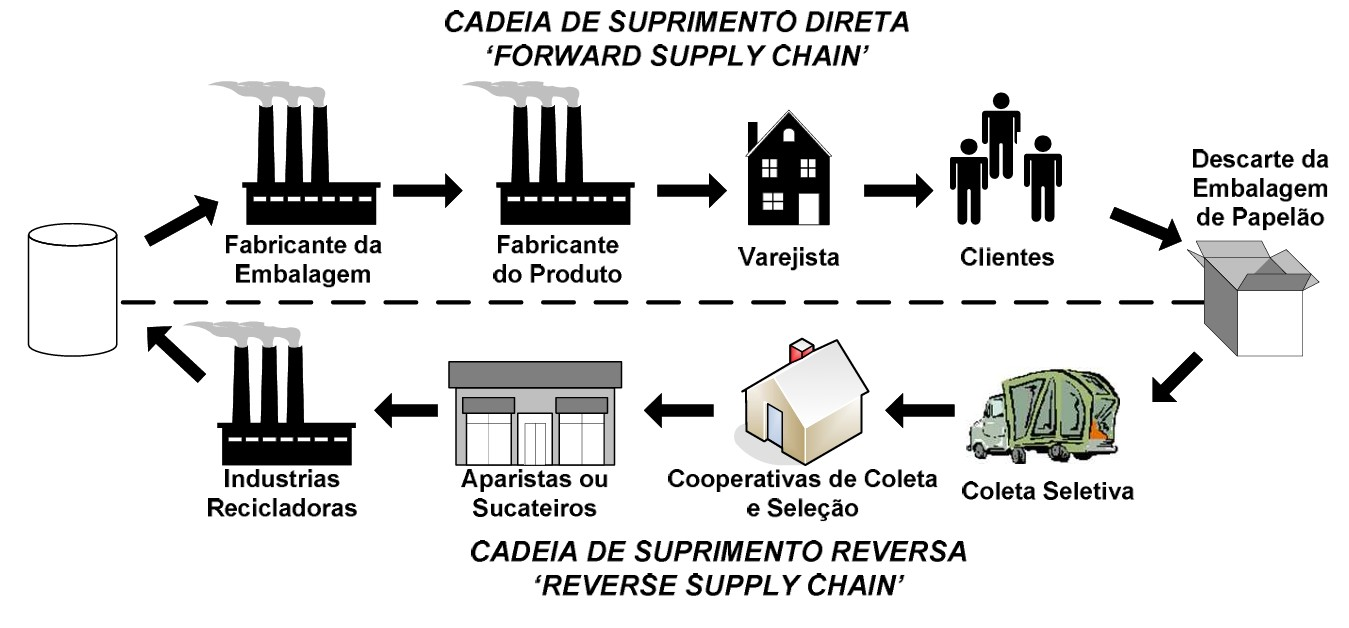
\includegraphics[width=15cm]{images/RF_img/Figura_CSCF.jpg}
	\end{center}
	\fdireta[p. 3]{Georges2009Cadeia}
\end{figure}

Neste caso foi utilizado como exemplo uma cadeia de suprimentos de embalagens, porém pode mudar algumas localidades conforme o tipo de negócio, mas o que não muda é o modelo.

Para \citeonline{GOVINDAN2015603}, devido a fatores ambientais, legais, sociais e econômicos, a CSCF passou a despertar grande interesse tanto na academia quanto no setor empresarial. Isso ocorre porque ela atua como um elemento integrador entre a logística direta e a logística reversa, sendo essencial para a recuperação de valor dos produtos e para o cumprimento de metas relacionadas à sustentabilidade.

A modelagem da CSCF é aplicável a diversos tipos de produtos, o que demonstra a versatilidade do modelo para diferentes contextos logísticos. Sua aplicação varia entre aqueles com a necessidade de um reuso rápido e constante, como o caso estudado por \citeonline{Avoleta2013Dimensionamento} sobre o dimensionamento de estoque de embalagens retornáveis. Em contraste, a CSCF também é pertinente para \textbf{bens duráveis} de longo ciclo de vida, como demonstrado na análise de \citeonline{Pereira2016Previsao} sobre a previsão de retorno de pneus inservíveis.

A CSCF, embora sua origem não esteja exclusivamente ligada a imperativos ambientais, demonstrou ser uma aliada estratégica fundamental. Ao integrar os fluxos da logística direta e da logística reversa, a CSCF permite a recuperação e valorização de materiais pós-consumo, gerando uma significativa vantagem competitiva para as empresas.

Essa evolução na gestão da cadeia converge diretamente com o conceito de \sigla{TBL}{Triple Bottom Line}, conhecido como o Tripé da Sustentabilidade. O TBL, conforme estabelecido por \citeonline{elkington1997triple}, representa a necessidade de gerenciar de forma integrada as três dimensões de desempenho: social (\emph{People}), ambiental (\emph{Planet}) e econômica (\emph{Profit}), de modo que a gestão do negócio não se restrinja à obtenção de lucros.

\subsection{A CSCF para Resíduos de Equipamentos Eletrônicos.}\label{A CSCF para Resíduos de Equipamentos Eletrônicos.}

Os motivos para a implementação da CSCF para REEE não é apenas o ambiental, além deste existe a motivação econômica e regulatória. Para, \citeonline{brito2002reverse} os motivos para investir em uma LR, e por consequência construir uma CSCF, são formadores do "triângulo de fatores" compostos pelos eixos:

\begin{itemize} 
    \item Econômico: engloba os benefícios obtidos por meio da reutilização e reciclagem de materiais, da recuperação de componentes de valor e de ganhos indiretos, como o fortalecimento da imagem da empresa por meio do marketing sustentável e a proteção estratégica, que impede o acesso de concorrentes a tecnologias ou processos produtivos próprios.
    \item Legislativo: refere-se ao conjunto de normas e obrigatoriedades a serem seguidas para redução de emissão de poluentes no meio ambiente. No contexto brasileiro, destaca-se a Política Nacional de Resíduos Sólidos, instituída pela Lei n\textordmasculine~12.305/2010 \cite{Lei12305_2010} e regulamentada pelo Decreto n\textordmasculine~10.936/2022 \cite{Decreto10936_2022}, que obriga as organizações a adotarem práticas sustentáveis ao longo de toda a sua cadeia produtiva.
    \item Responsabilidade Estendida: refere-se aos princípios éticos e de sustentabilidade que orientam as empresas a se engajarem efetivamente no desenvolvimento sustentável e na redução de impactos ambientais.    
\end{itemize}

\begin{figure}[htb]
	\caption{Triângulo de fatores.}\label{fig_tr_fat}
	\begin{center}
        \includegraphics[width=10cm]{images/RF_img/Triangulo_de_Fatores.png}
	\end{center}
	\fdireta[p. 7]{brito2002reverse}
\end{figure}

Outro ponto relevante ao tratar dos REEE diz respeito às suas características de deterioração dos itens. Muitos desses equipamentos, como telefones móveis, possuem vida útil relativamente curta, pois grande parte dos usuários utilizam por apenas dois anos. Além disso, destaca-se a possibilidade de reparabilidade, que permite o conserto e o reaproveitamento de componentes, prolongando a utilização dos produtos. Por fim, há a obsolescência programada é a limitação artificial da durabilidade dos bens manufaturados, com o intuito de incentivar o consumo repetido \cite{YlaMella2022EndofUse}.

Considerando as características de deterioração, a CSCF aplicada aos REEE envolve algumas etapas fundamentais. A primeira é a coleta, que consiste na remoção dos itens junto aos clientes, pontos de coleta, lojas e outros locais de descarte. Em seguida, ocorre a triagem, etapa em que os produtos são desmontados, separados, compactados, armazenados ou avaliados quanto ao potencial de reutilização. A fase de reprocessamento corresponde à transformação dos materiais em insumos que possam ser novamente utilizados. Por fim, ocorre a reinserção, que envolve a recomercialização do item ou do subproduto obtido por meio da reciclagem, reintegrando-o ao ciclo produtivo \cite[apud Mendes, 2017]{pereira2018logistica}.

\section{Problemas de Localização de Facilidades na Cadeia Logística}\label{Problemas de localização e alocação de facilidades na cadeia logística}
Problemas de localização e alocação de facilidades é uma das linhas de pesquisa que se desenvolvem metodologias na área logística, pode-se verificar a grande importância do assunto quando se verifica o caso da empresa \emph{Leaseway Transportation Corporation}, em que foi utilizado a metodologia de Localização de Alocação de Facilidades conhecida como Centro de Gravidade. Com esta aplicação a companhia conseguiu definir a localização de uma instalação de manutenção de caminhões em Boston \cite{ballou2006gerenciamento}.

Segundo \citeonline{arakaki2006heuristica}, a FLP é um aspecto crítico no planejamento estratégico para um grande espectro de empresas públicas e privadas. Seja um empresário que quer construir um novo shopping, um industrial que deseja situar uma nova fábrica ou um administrador público que quer estabelecer postos de saúde, são frequentemente desafiados pela dificuldade de decidir por um local adequado, com isso percebe-se o grande valor que possui este tipo de estudo, podendo se tornar um diferencial competitivo.

Muitas vezes, este estudo deve contar com a Pesquisa Operacional (PO) como suporte para os cálculos necessários a fim de encontrar a melhor solução possível, ou com a função objetivo (FO). Um exemplo disso é o estudo de \citeonline{medrano2020using}, que define um problema de localização de máxima cobertura para a LR de produtos no fim do ciclo de vida, onde a PO foi utilizada para a execução das análises. Além disso, é importante ressaltar que a LR também fará parte desta dissertação de mestrado.

Para gestão de resíduos e recuperação de materiais, o planejamento de FLP é de grande criticidade, pois a definição de quantidade de facilidades e suas localizações possuem um impacto enorme na eficiência de transportes, \citeonline{TOSO2014839} demonstram a possibilidade da aplicação de dois modelos, um determinístico e um estocástico para se obter uma solução ótima.

\section{Programação Linear Inteira Mista (PLIM)}

A técnica de PLIM caracteriza-se pela presença simultânea de variáveis de decisão contínuas e discretas. As variáveis contínuas podem representar, por exemplo, a quantidade de movimentações de itens ou o nível de estoque em um CSCF, enquanto as variáveis discretas estão associadas à ativação de localidades, modeladas por meio de variáveis binárias. Segundo \citeonline{Camelo2024}, o PLIM se destaca por fornecer ferramentas para o planejamento logístico, integrando de maneira eficiente decisões estratégicas e operacionais em cadeias de suprimentos complexas voltadas para o hidrogênio verde.

Por se tratar de uma abordagem de PO, a modelagem por PLIM envolve três componentes fundamentais: a função objetivo, que define o propósito da otimização — podendo ser de maximização ou minimização; as variáveis de decisão, determinadas pela formulação computacional do modelo, que podem ser contínuas, inteiras ou binárias; e os conjuntos de restrições, que representam limitações como capacidades, regras de negócio, localizações pré-definidas, entre outras. Essa estrutura é exemplificada em \citeonline{Guzman2023Matheuristic}, que propõem um modelo de PLIM voltado à minimização dos custos de produção, estoque, transporte e atraso. O modelo considera variáveis de decisão como nível de estoque, quantidade de produtos transportados e produzidos, e ativação de plantas industriais, utilizando parâmetros como custos unitários de transporte, produção e armazenagem, demanda, capacidades máximas de estoque e custo de abertura.

A PLIM é amplamente empregada em modelos de localização de CDs e PAs, bem como no dimensionamento de estoques em CSCF. Segundo \citeonline{Vicente2025}, que aplica a PLIM na revisão periódica de estoques de uma cadeia de suprimentos com múltiplos estágios, os resultados obtidos indicam melhorias significativas na configuração da rede e redução expressiva de custos operacionais de pedido, transportes e manutenção.

Neste trabalho, ao abordar a CSCF de adquirência, que inclui a presença de CDs, PAs, além de fluxos diretos e reversos, a representação do problema por meio de um modelo PLIM é escolhida, pois permite modelar tanto variáveis binárias quanto variáveis contínuas, tudo inserido no contexto de uma função objetivo de minimização do custo total. Estudos recentes corroboram com esta escolha como é o caso de \citeonline{Oujana2023} que utilizam a mesma abordagem  para resolução de sistemas complexos de agendamento de produção, distribuição e estoques de uma planta de embalagens.

\chapter{Definição do Problema e Modelagem Matemática}
\label{chapter:def_prob_mod}
\section[Contextualização da Empresa de Adquirência]{Contextualização da Empresa de Adquirência}
\label{Tecnologias}

Uma empresa de adquirência é o ramo que se responsabiliza pelo gerenciamento e operação de máquinas de transações via cartões (crédito e débito), tendo uma operação muito complexa no que se refere a logística, pois possui atendimento geográfico amplo através de seus CDs e postos avançados que são responsáveis pela distribuição de máquinas para seus clientes.

Este ramo empresarial está em constante crescimento. Segundo o Banco Central Brasileiro, o número de transações realizadas no Brasil em 2011 foi de 3,83 milhões. Em 2020, houve um aumento significativo, atingindo 9,67 milhões de transações. Ao considerarmos os cartões de crédito ativos para os mesmos anos, em 2011 havia 78,4 milhões e em 2020 esse número subiu para 133,7 milhões. Isso indica que quanto mais cartões existem, maior é a quantidade de máquinas que devem estar disponíveis no mercado para realizar pagamentos e transações eletrônicas \cite{TNS}.

Em 2020, os pagamentos feitos utilizando cartões de crédito, débito ou pré-pago foi de R\$ 2 trilhões, informa a Associação Brasileira das Empresas de Cartões de Crédito e Serviços (Abecs). Este valor é equivalente a 27\% do PIB brasileiro \cite{Valenti1998}. Estes números corroboram com o aumento do mercado consumidor e do quanto o mercado de adquirência se torna cada dia mais importante em um mercado que exige agilidade, facilidade e segurança em transações de crédito eletrônico.

No setor de adquirência, o elevado volume de transações confere à logística uma importância estratégica para a economia. Dessa forma, a gestão logística deve ser tratada com rigor, abrangendo não apenas os equipamentos em si, mas também todos os seus componentes críticos, como o \emph{SIM card} e os \emph{microchips} responsáveis pela conexão das máquinas à rede de internet. Em sua pesquisa, \citeonline{Silva2021Adquirencia} demonstra que mesmo ativos de baixo custo, como o \emph{SIM card}, possuem alta criticidade operacional, evidenciando que a complexidade do estudo logístico é essencial para a eficiência do setor.

Hoje em dia, a maioria dos estabelecimentos possuem uma máquina de cartão, desde profissionais autônomos a grandes empresas varejistas e de prestação de serviço. O pagamento por meio eletrônico é uma segurança tanto para o cliente, quanto para o consumidor, pois o cliente não precisa portar consigo dinheiro em espécie e o para o estabelecimento é uma garantia que irá receber corretamente, sem risco de receber dinheiro falso. Portanto, este é o motivo de sua consolidação no mercado.

Os produtos comercializados pela empresa de adquirência são máquinas de transações eletrônicas, que de uma maneira geral compõem a cadeia logística com dois tipos de tecnologia, sendo POS e PINPAD.

A tecnologia de POS é a máquina que usualmente se encontra nos estabelecimentos comuns, como açougue, ambulantes, pequenos e médios varejistas. A tecnologia PINPAD é utilizada nos grandes varejistas e exigem a configuração de um software em um microcomputador (\autoref{fig_pos_pinpad}).

\begin{figure}[htb]
	\caption{ máquina POS (2) e PINPAD (3)}\label{fig_pos_pinpad}
	\begin{center}
            \includegraphics[width=1.04cm]{images/RF_img/POS.png}
            (2) \hspace{1cm} \includegraphics[width=2cm]{images/RF_img/PINPAD.png}
            (3)
	\end{center}
	\fdadospesquisa
\end{figure}

\section[Descrição do Problema de Otimização]{Descrição do Problema de Otimização}
\label{Descrição do Problema}
O caso em estudo considera a FLP motivada por um problema enfrentado por uma empresa brasileira de adquirência. O foco do estudo está para as facilidades existentes em todo o território brasileiro, levando em consideração apenas a distribuição de máquinas POS.

Uma empresa de adquirência, em geral, adota um modelo logístico integrado para sua distribuição, englobando os processos de \emph{inbound}, \emph{outbound}, armazenagem e distribuição de produtos:

\begin{itemize}
    \item \emph{Inbound}: A entrada de produtos ocorre com o abastecimento dos CDs pelos fabricantes, que enviam tanto novas máquinas quanto máquinas reparadas, assegurando que estejam em boas condições para uso.

    \item \emph{Outbound}: O fluxo de saída de produtos inclui a movimentação dos CDs para os PAs e, por fim, do PA até o cliente final. Esse fluxo garante que os produtos necessários estejam disponíveis para atender à demanda na ponta da cadeia.

    \item Armazenagem: 
        \begin{itemize}
            \item CDs: Em geral, os CDs são estabelecidos em menor quantidade devido ao seu tamanho e capacidade de armazenagem. Eles mantêm uma grande variedade de produtos e são responsáveis por abastecer os PAs, cumprindo a função principal de estoque centralizado na rede logística.
            \item PAs: Localizados em maior quantidade, os PAs possuem uma área reduzida de armazenamento e servem para manter estoques próximos dos clientes em regiões específicas. Esses pontos permitem uma resposta mais ágil às necessidades dos clientes em áreas com alta ou baixa densidade populacional.
        \end{itemize}

    \item Distribuição: A distribuição envolve o transporte dos produtos do CD até os PAs e, em seguida, o abastecimento dos clientes finais. Os clientes são o destino final da cadeia, onde as transações financeiras ocorrem e geram receita para a empresa.
\end{itemize}

Além disso, outros elementos importantes para manter o abastecimento na cadeia logística são:

\begin{itemize}
    \item Fabricantes: São responsáveis pelo abastecimento dos CDs com novos produtos e máquinas reparadas, garantindo o ciclo contínuo de reposição e manutenção dos equipamentos da rede logística.
    
    \item Empresa de descartes: Especializada em descarte de produtos eletrônicos com certificação ISO14001, recebe itens que não podem mais ser reutilizados na cadeia. Produtos com avarias irreparáveis ou cujo remanufatura é inviável financeiramente são enviados para essas empresas, atendendo aos padrões ambientais de descarte.
\end{itemize}

Uma característica essencial na rede logística de uma empresa de adquirência é que ela opera dentro de uma CSCF, ou seja, os itens enviados ao cliente retornam pelos mesmos canais de distribuição, caracterizando a LR. Assim, o produto é enviado e retorna de forma contínua, não havendo um "fim" para o item, a menos que ele se torne impróprio para reutilização. Nesse fluxo, todo o processo é empurrado, exceto nas etapas realizadas nos PAs, onde a demanda de instalação e desinstalação ocorre de forma puxada.

O envio das máquinas inicia-se com o fabricante. Esse envio ocorre de duas maneiras: a primeira é com a compra por parte da adquirência, geralmente envolvendo negociações por lote e em grande quantidade, momento em que o fabricante envia as máquinas para o CD. A segunda maneira é pela reversão de máquinas quebradas, que precisam de remanufatura especializado, oriundas dos CDs, e, após o remanufatura, são enviadas novamente aos CDs.

Os CDs, por sua vez, são abastecidos pelos fabricantes e pelas máquinas retornadas dos PAs, formando um estoque disponível, que é enviado aos PAs conforme a demanda de pedidos.

Os PAs são a última etapa do processo antes de enviar a máquina para o cliente e a primeira etapa da reversa, após a desinstalação da máquina no cliente. Entretanto, não existe nenhuma ação de manutenção nesses PAs, ou seja, a máquina não passa por remanufaturas nesta etapa. Existem PAs maiores, mas, na grande maioria, são locais que muitas vezes podem ser uma casa residencial que se tornou um PA.

A distribuição no PA ocorre conforme a demanda do cliente. Ou seja, o cliente utiliza uma das plataformas disponíveis para solicitar a instalação, e, então, é criado um número de ordem de serviço, e o PA deve enviar e instalar a máquina dentro de um prazo determinado, conforme a região.

A operação de reversão se inicia no posto avançado, iniciada pelo cliente, que abre uma ordem de serviço para desinstalação, na mesma plataforma de solicitação de instalação. Em seguida, o PA remove a máquina do cliente e a armazena para posterior envio aos CDs.

Tanto o envio quanto o recolhimento das máquinas ocorrem por meio de técnicos aptos a instalar e desinstalar as máquinas, e o transporte utilizado pode ser tanto motocicleta quanto veículos utilitários, conforme a demanda.

O processo de reversa dos PAs para os CDs ocorre por meio de agendas semanais pré-definidas, podendo, em alguns locais, ocorrer o \emph{milk run}, em que um veículo passa por vários PAs recolhendo as máquinas até chegar ao CD.

Ao retornarem ao CD, as máquinas passam pelo processo de recebimento e triagem, que funcionam praticamente como uma única etapa. Na triagem, são realizadas pequenas manutenções, como a troca de tampa de bateria, além de limpeza, garantindo que estejam em condições de atender a um novo cliente. Caso a máquina exija reparos mais complexos, como a substituição da tela de LED, ela é enviada aos fabricantes, que oferecem serviços de remanufatura. Se for determinado que a máquina não pode ser reutilizada, ela retorna ao CD, que a encaminha a uma empresa especializada no descarte de materiais eletrônicos. No entanto, o número de máquinas destinadas ao descarte é muito baixo, o que permite que esse processo seja, na prática, desconsiderado.

O fluxo no CD se inicia pelo recebimento. Se a máquina for oriunda da reversa (postos avançados), ela passa por um processo de triagem. Se a origem for o fabricante, a máquina é enviada para a armazenagem para posterior avanço aos PAs. Após passar pela triagem no CD, se a máquina estiver apta, ela segue para a armazenagem.

No que diz respeito ao controle das movimentações das máquinas, uma equipe de gestão de ativos é responsável por todo o acompanhamento e controle. Cada máquina possui um registro único (código de barras), o que garante sua rastreabilidade ao longo de seu ciclo de vida. As máquinas têm uma vida útil estimada em torno de 5 anos. Para o controle dos estoques, é realizado um inventário oficial anual, além de inventários rotativos ao longo do ano, conforme a necessidade.

O cliente recebe a máquina no modelo de comodato, sem custo inicial, mediante pagamento de um aluguel mensal. Toda essa rede logística é importante para garantir que a máquina esteja disponível no cliente, facilitando a geração de receita tanto para o cliente quanto para a empresa. Além disso, cada transação realizada na máquina está sujeita a uma taxa administrativa cobrada pela adquirente, sendo que o valor a ser repassado ao cliente é sempre descontado do valor do aluguel mensal.

A estrutura de uma companhia de adquirência pode ser melhor observada conforme (\autoref{fig_fluxo_complexo}) e o processo interno do CD (\autoref{fig_fluxo_cd}).

\begin{figure}[htb]
	\caption{Fluxo logístico (\emph{inbound}, armazenagem, distribuição e \emph{outbound}) de fluxo fechado}\label{fig_fluxo_complexo}
	\begin{center}
            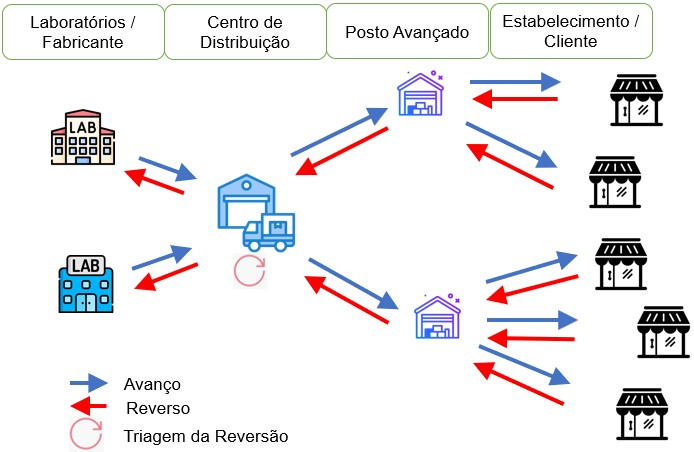
\includegraphics[width=10cm]{images/RF_img/FluxoLogisticoCompleto.jpg}
	\end{center}
	\fdadospesquisa
\end{figure}

\begin{figure}[htb]
	\caption{\label{fig_fluxo_cd} Fluxo de processo no CD}
	\begin{center}
            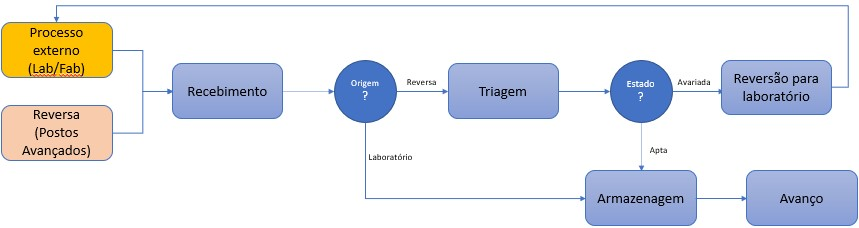
\includegraphics[width=10cm]{images/RF_img/FluxoCD.jpg}
	\end{center}
	\fdadospesquisa
\end{figure}

Uma característica importante a ser considerada é que, devido a restrições fiscais, o fluxo logístico entre CDs, PAs e clientes segue uma estrutura fixa, sem sobreposição. Isso significa que uma máquina enviada de um CD específico, passando por um PA até o cliente, deve retornar pelo mesmo caminho no fluxo reverso, passando pelo mesmo PA e CD de origem. Devido a essa restrição, cada CD atende um grupo fixo de PAs, sem alterações ao longo do tempo. Nas fábricas, embora a regra de não sobreposição também se aplique, uma única fábrica pode atender a todos os CDs, desde que respeite essa configuração de origem e destino.

Seguindo a lógica da não sobreposição, considera-se um problema motivado por uma empresa que conta, por exemplo, com duas fábricas na região de Osasco/SP e três CDs: Araucária/PR (CD Araucária), Jaboatão dos Guararapes/PB (CD Jaboatão) e Guarulhos/SP (CD GRU). Além disso, considere que o CD Araucária atende exclusivamente à região Sul, o CD Jaboatão atende às regiões Norte e Nordeste, e o CD GRU atende às regiões Sudeste e Centro-Oeste. A rede conta com aproximadamente duzentos PAs, distribuídos da seguinte forma: 20\% na região Sul, 30\% nas regiões Norte e Nordeste, e os 50\% restantes nas demais regiões. Os clientes atendidos pelos PAs são segmentados em ZDs sem sobreposição, conforme (\autoref{fig_mapa_brasil_redelog}). Em outras palavras, cada grupo de estabelecimentos forma uma ZD atendida por apenas um PA específico.

\begin{figure}[htb]
	\caption{Distribuição geográfica do fluxo logístico}\label{fig_mapa_brasil_redelog}
	\begin{center}
            \includegraphics[width=10cm]{images/RF_img/MapaCDSEREGIAO.png}
	\end{center}
	\fdadospesquisa
\end{figure}


Para atender à demanda, a rede logística mantém um estoque amplo de máquinas, além das unidades já instaladas, em trânsito ou em processos de reparo e remanufatura. Esse estoque garante uma cobertura total de 90 dias. Em outras palavras, mesmo sem reposição, a rede possui capacidade para abastecer seus clientes durante esse período.

\section[Formulação do Modelo PLIM]{Formulação do Modelo PLIM}\label{modeloproposto}
\label{Modelagem Matemática}

\noindent \textbf{Índices e Parâmetros}


%\subsection{Índices e Parâmetros}

$I$ = conjunto de Centros de Distribuição (CDs) indexado por $i$;

$J$ = conjunto de Zonas de Demanda (ZDs) indexado por $j$;

$P$ = conjunto de Postos Avançados (PAs) indexado por $p$;

$L$ = conjunto de Fabricantes indexado por $l$;

$D$ = conjunto de Unidades de Descarte indexado por $d$;

$T$ = conjunto de Períodos de Tempo em meses indexado por $t$.

Parâmetros para o fabricante:

$m^{rf}_{l}$: capacidade de processamento do fabricante l $\in$ L (nº de máquinas);

$m^{af}_{l}$: capacidade de expedição de material no fabricante $\in$ L (nº máquinas);

$e^{f}_{l,t}$: capacidade de estocagem do fabricante l $\in$ L (nº máquinas), por um período t $\in$ T;

$c^{fc}_{l,i}$: parâmetro indicação se o CD i $\in$ I e o fabricante l $\in$ L se localizam na mesma região \{0, 1\};

$d^{fc}_{l,i}$: distância em quilômetros entre o fabricante l $\in$ L e o CD i $\in$ I;

$r^{f}$: Taxa de produtos que precisam de remanufatura pelo fabricante \( l \in L, \), sendo \( 0 \leq rc \leq 1 \).

Parâmetros para os CDs:

$n^{c}$: máxima quantidade de CDs;

$m^{rc}_{i}$: capacidade de recebimento e triagem do CD i $\in$ I (nº de máquinas);

$m^{ac}_{i}$: capacidade de expedição de material do CD i $\in$ I (nº máquinas);

$e^{c}_{i,t}$: capacidade de estocagem do CD i $\in$ I (nº de máquinas) pelo período t $\in$ T;

$c^{cd}_{i,d}$: parâmetro de indicação se o CD i $\in$ I e o descarte d $\in$ D se localizam na mesma região \{0, 1\};

$c^{cp}_{i,p}$: parâmetro indicação se o CD i $\in$ I e o PA p $\in$ P se localizam na mesma região \{0, 1\};

$d^{cd}_{i,d}$: distância em quilômetros entre o CD i $\in$ I e o descarte d $\in$ D;

$d^{cp}_{i,p}$: distância em quilômetros entre o CD i $\in$ I e o PA p $\in$ P;

$r^{c}$: taxa de produtos, bons para reutilização, devolvidos no CD \( i \in I \), sendo \( 0 \leq rc \leq 1 \);

$\theta^{c}$: taxa mínima de retenção de estoque de itens bons nos Centros de Distribuição (CDs), fixada em 65\% conforme diretriz da empresa, utilizada como uma \textit{proxy} operacional para a manutenção de uma política de cobertura de estoque de 90 dias.

Parâmetros para os PAs:

$n^{p}$: máxima quantidade de PAs;

$m^{rp}_{p}$: capacidade de recebimento do PA p $\in$ P (número de maquinetas);

$m^{ap}_{p}$: capacidade de expedição do PA p $\in$ P (nº maquinetas);

$e^{p}_{p,t}$: capacidade de estocagem do PA p $\in$ P (nº de maquinetas) pelo período t $\in$ T;

$c^{pj}_{p,j}$: parâmetro de indicação se o PA p $\in$ P e a ZD j $\in$ J se localizam na mesma região \{0, 1\};

$d^{pj}_{p,j}$: distância em quilômetros entre o PA p $\in$ P e a ZD j $\in$ J;

$\theta^{p}$: taxa mínima de retenção de estoque nos Postos Avançados (PAs), fixada em 50\% conforme diretriz da empresa, utilizada como uma \textit{proxy} de segurança operacional para garantir o abastecimento contínuo das Zonas de Demanda (ZDs).

Parâmetro para as ZDs:

$dem^{rj}_{j,t}$: demanda de máquinas para desinstalação na ZD j $\in$ J;

$dem^{aj}_{j,t}$: demanda de máquinas para instalação na ZD j $\in$ J;

$BM$: parâmetro \emph{Big} M;

Em PLIM, o \textit{Big} M é um artifício matemático usado para vincular uma variável contínua (ex: quantidade de envio) a uma variável binária. A restrição com o \textit{Big} serve para impor a seguinte lógica: não pode haver fluxo de itens (maquinetas) saindo ou chegando a um local que não esteja aberto.

\noindent \textbf{Variáveis de decisão}

%\subsection{Variáveis de decisão}

Variáveis para fábricas:

%$b^{fc}_{l,i}$: indicação se o CD i $\in$ I é atendido pelo fabricante l $\in$ L, sendo \{0, 1\};
$q^{ac}_{l,i,t}$: quantidade de máquinas enviadas do fabricante l $\in$ L para o CD i $\in$ I no período t $\in$ T;

$q^{fra}_{l,t}$: quantidade de máquinas enviadas do estoque de reversa para o estoque de avanço no fabricante l $\in$ L no período t $\in$ T;

$q^{f}_{l,t}$: quantidade de máquinas novas que entram para compor o estoque de máquinas prontas para uso no fabricante l $\in$ L no período t $\in$ T;

$s^{f}_{l,t}$: quantidade de máquinas que compõe o estoque do fabricante l $\in$ L em um período t $\in$ T;

$s^{frf}_{l,t}$: quantidade de máquinas da reversa que compõe o estoque do fabricante l $\in$ L em um período t $\in$ T;

$s^{fbc}_{l,t}$: quantidade para avanço que compõe o estoque do fabricante l $\in$ L em um período t $\in$ T;

Variáveis para os CDs:

$o^{c}_{i,t}$: indica se o CD i $\in$ I está aberto no período t $\in$ T, sendo \{0, 1\};

$b^{cp}_{i,p,t}$: indicação se o PA p $\in$ P é atendido pelo CD i $\in$ I, sendo \{0, 1\};

$b^{cd}_{i,d,t}$: indicação se o CD i $\in$ I é atendido pelo descarte d $\in$ D no período t $\in$ T, sendo \{0, 1\};

$q^{rf}_{i,l,t}$: quantidade de máquinas enviadas do CD i $\in$ I para o fabricante l $\in$ L no período t $\in$ T;

$q^{ap}_{i,p,t}$: quantidade de máquinas enviadas do CD i $\in$ I para o PA p $\in$ P no período t $\in$ T;

$q^{rd}_{i,t}$: quantidade de máquinas enviadas do CD i $\in$ I para ser descartado, no período t $\in$ T;

$s^{c}_{i,t}$: quantidade de máquinas que compõe o estoque do CD i $\in$ I no período t $\in$ T no período t $\in$ T;

$s^{crf}_{i,t}$: quantidade de máquinas da reversa para envio ao fabricante que compõe o estoque do CD i $\in$ I no período t $\in$ T no período t $\in$ T;

$s^{crd}_{i,t}$: quantidade de máquinas da reversa para envio para descartes que compõe o estoque do CD i $\in$ I no período t $\in$ T no período t $\in$ T;

$s^{cbp}_{i,t}$: quantidade de máquinas para avanço que compõe o estoque do CD i $\in$ I no período t $\in$ T no período t $\in$ T;

$s^{cbt}_{i,t}$: quantidade de máquinas em estoque transitório que compõe o estoque do CD i $\in$ I no período t $\in$ T no período t $\in$ T;

$z_{i,t}$: indica se ocorre a primeira abertura do CD i $\in$ I no período t $\in$ T;

Variáveis para os PAs:

$o^{p}_{p,t}$: indica se o PA p $\in$ P está aberto no período t $\in$ T, sendo \{0, 1\};

$b^{pj}_{p,j,t}$: indicação se a ZD j $\in$ J é atendida pelo PA p $\in$ P no período t $\in$ T, sendo \{0, 1\};

$q^{rc}_{p,i,t}$: quantidade de máquinas enviadas do PA p $\in$ P para o CD i $\in$ I no período t $\in$ T;

$q^{aj}_{p,j,t}$: quantidade de máquinas enviadas do PA p $\in$ P para a ZD j $\in$ J no período t $\in$ T;

$s^{p}_{p,t}$: quantidade de máquinas que compõe o estoque do PA p $\in$ P no período t $\in$ T;

$s^{prc}_{p,t}$: quantidade de máquinas para reversa que compõe o estoque do PA p $\in$ P no período t $\in$ T;

$s^{pbj}_{p,t}$: quantidade de máquinas para avanço que compõe o estoque do PA p $\in$ P no período t $\in$ T;

$w_{i,t}$: indica se ocorre a primeira abertura do PA i $\in$ I no período t $\in$ T;

Variáveis para ZDs:

$q^{rp}_{j,p,t}$: quantidade de máquinas enviadas da ZD j $\in$ J para o PA p $\in$ P no período t $\in$ T;

Custos:

$k$: custo por quilometragem por máquina;

$h_{i}$: custo abertura CD;

$u_{p}$: custo abertura PA;

$v_{i}$: custo de manutenção CD;

$x_{p}$: custo de manutenção PA.


\noindent \textbf{Função Objetivo (Minimização de Custos)}


%\subsection{Função Objetivo (Minimização de Custos)}

\begin{equation}\label{fo}
\begin{aligned}
\min Z = & \sum_{t=1}^{T} \left( \sum_{i=1}^{I} z_{i,t} \cdot h_{i} + \sum_{p=1}^{P} u_{p} \cdot w_{p,t} + \sum_{i=1}^{I} o^{c}_{i,t} \cdot v_{i} + \sum_{p=1}^{P} x_{p} \cdot o^{p}_{p,t} \right.\\
& + \sum_{l=1}^{L}\sum_{i=1}^{I} q^{ac}_{l,i,t} \cdot d^{fc}_{l,i} \cdot k + \sum_{i=1}^{I}\sum_{l=1}^{L} q^{rf}_{i,l,t} \cdot d^{fc}_{l,i} \cdot k \\
& + \sum_{i=1}^{I}\sum_{p=1}^{P} q^{ap}_{i,p,t} \cdot d^{cp}_{i,p} \cdot k + \sum_{i=1}^{I}\sum_{l=1}^{L} q^{rc}_{p,i,t} \cdot d^{cp}_{i,p} \cdot k \\
& + \sum_{i=1}^{I}q^{rd}_{i,t} \cdot d^{cd}_{i,d} \cdot k + \sum_{p=1}^{P}\sum_{j=1}^{J} q^{aj}_{p,j,t} \cdot d^{pj}_{p,j} \cdot k \\
& \left. + \sum_{j=1}^{J}\sum_{p=1}^{P} q^{rp}_{j,p,t} \cdot d^{pj}_{p,j} \cdot k \right) \quad t \in T
\end{aligned}
\end{equation} 

% =================================================================
% COMPONENTES DA FUNÇÃO OBJETIVO
% =================================================================

A função objetivo (\ref{fo}) visa minimizar o custo logístico total da rede, sendo estruturada pela soma de três componentes principais. O custo de instalação (\ref{cinst}) contabiliza as despesas fixas incidentes apenas sobre a decisão binária de abertura de novas facilidades (CDs e PAs). O custo de manutenção (\ref{cmanut}) agrega as despesas operacionais recorrentes de cada facilidade mantida ativa durante o horizonte de planejamento. Por fim, o custo de transporte (\ref{ctransp}) quantifica o gasto logístico de movimentação, calculado pelo produto entre o custo unitário por quilômetro, a distância entre os nós e o volume de equipamentos (fluxo) transferidos.

% Custo de Instalação (Instalação Inicial - Abertura)
\begin{equation}\label{cinst}
\sum_{t \in T} \left( \sum_{i \in I} z_{i,t} \cdot h_{i} + \sum_{p \in P} w_{p,t} \cdot u_{p} \right)
\end{equation}

% Custo de Manutenção (Custo Operacional Recorrente)
\begin{equation}\label{cmanut}
\sum_{t \in T} \left( \sum_{i \in I} o^{c}_{i,t} \cdot v_{i} + \sum_{p \in P} o^{p}_{p,t} \cdot x_{p} \right)
\end{equation}

\begin{equation}\label{ctransp}
\begin{aligned}
& \sum_{l=1}^{L}\sum_{i=1}^{I} q^{ac}_{l,i,t} \cdot d^{fc}_{l,i} \cdot k + \sum_{i=1}^{I}\sum_{l=1}^{L} q^{rf}_{i,l,t} \cdot d^{fc}_{l,i} \cdot k \\
& + \sum_{i=1}^{I}\sum_{p=1}^{P} q^{ap}_{i,p,t} \cdot d^{cp}_{i,p} \cdot k + \sum_{i=1}^{I}\sum_{l=1}^{L} q^{rc}_{p,i,t} \cdot d^{cp}_{i,p} \cdot k \\
& + \sum_{i=1}^{I}q^{rd}_{i,t} \cdot d^{cd}_{i,d} \cdot k + \sum_{p=1}^{P}\sum_{j=1}^{J} q^{aj}_{p,j,t} \cdot d^{pj}_{p,j} \cdot k \\
& + \sum_{j=1}^{J}\sum_{p=1}^{P} q^{rp}_{j,p,t} \cdot d^{pj}_{p,j} \cdot k
\end{aligned}
\end{equation}

\noindent \textbf{Restrições do Modelo}

%\subsection{Restrições do Modelo}

\renewcommand{\theequation}{\arabic{chapter}.\arabic{equation}} % Comando para formatação da numeração se necessário.

% =========================================================
% RESTRIÇÕES DOS FABRICANTES
% =========================================================
Restrições de fábrica:

As restrições (\ref{re1}) garantem que a capacidade máxima de processamento (operações de remanufatura) em cada fabricante, originados do CD, não seja excedida.

\begin{equation}\label{re1}
\sum_{i=1}^{I} q^{rf}_{i,l,t} \leq m^{rf}_{l} \quad \forall l \in L, \quad \forall t \in T
\end{equation}

As restrições \ref{re2} garantem que a capacidade máxima de expedição de itens bons pelo fabricante aos CDs, não seja excedida.
\begin{equation}\label{re2}
\sum_{i=1}^{I} q^{ac}_{l,i,t} \leq m^{af}_{l} \quad \forall l \in L, \quad \forall t \in T
\end{equation}

As restrições \ref{re3} garantem a composição total de estoque de máquinas no fabricante, estoque de itens para remanufatura e estoque de itens reparados, para envio aos CDs.
\begin{equation}\label{re3}
\begin{aligned}
& s^{f}_{l,t} = s^{fbc}_{l,t} + s^{frf}_{l,t} \quad & \forall l \in L, \quad \forall t \in T
\end{aligned}
\end{equation}

As restrições \ref{re4} garantem o balanceamento do estoque de itens a serem reparados, para conserto, no fabricante, sendo composto pelo recebimento do dos itens enviados pelos CDs, subtraído do envio de itens que foram consertados e enviados para o estoque de itens bons, somado do estoque do período anterior.
\begin{equation}\label{re4}
\begin{aligned}
& \sum_{i=1}^{I} q^{rf}_{i,l,t} - q^{fra}_{l,t} + s^{frf}_{l, t-1} = s^{frf}_{l, t} \quad & \forall l \in L, \quad \forall t \in T
\end{aligned}
\end{equation}

As restrições \ref{re5} garantem o balanceamento do estoque de itens bons envio do fabricante ao CD, sendo composto pela quantidade de itens consertados no próprio fabricante, subtraído pela quantidade de itens enviadas aos CDs, somado da quantidade do estoque do período anterior .
\begin{equation}\label{re5}
\begin{aligned}
& q^{fra}_{l,t} - \sum_{i=1}^{I} q^{ac}_{l,i,t} + q^{f} + s^{fbc}_{l, t-1} = s^{fbc}_{l, t} \quad & \forall l \in L, \quad \forall t \in T
\end{aligned}
\end{equation}

As restrições \ref{re6} garantem que o estoque no fabricante não seja maior que sua capacidade.
\begin{equation}\label{re6}
s^{f}_{l,t} \leq e^{f}_{l} \quad \forall l \in L, \quad \forall t \in T
\end{equation}

As restrições \ref{ref2_5}  para envio ao CD, garantindo que apenas haja envio ao CD, se o mesmo estiver aberto.
\begin{equation}\label{ref2_5}
q^{ac}_{l,i,t} \leq BM \cdot o^{c}_{i, t} \quad \forall l \in L, \quad \forall i \in I, \quad \forall t \in T
\end{equation}

% =========================================================
% RESTRIÇÕES DOS CDS
% =========================================================

Restrições dos CDs:

As restrições \ref{re7} garantem que a capacidade máxima de recebimento e triagem no CD não seja excedida pela soma da quantidade de itens enviados do fabricante e dos PAs para os CDs.

\begin{equation}\label{re7}
\sum_{l=1}^{L} q^{ac}_{l,i,t} + \sum_{p=1}^{P} q^{rc}_{p,i,t} \leq m^{rc}_{i} \quad \forall i \in I, \quad \forall t \in T
\end{equation}

As restrições \ref{re8} garantem que a capacidade máxima de envio no CD não seja excedida, através da soma das quantidades de máquinas enviadas do CD para os fabricantes, para os PAs e para o descarte.
\begin{equation}\label{re8}
\sum_{l=1}^{L} q^{rf}_{i,l,t} + \sum_{p=1}^{P} q^{ap}_{i,p,t} + q^{rd}_{i,t}\leq m^{ac}_{i} \quad \forall i \in I, \quad \forall t \in T
\end{equation}

As restrições \ref{re9} garantem a composição de estoque total no CD, sendo composta pela somatória de estoque de itens ruins para envio para descarte, de itens para conserto para envio ao fabricante e de itens bons para envio aos PAs.
\begin{equation}\label{re9}
\begin{aligned}
& s^{crd}_{i,t} + s^{crf}_{i,t} + s^{cbp}_{i,t} + s^{cbt}_{i,t} = s^{c}_{i,t} \quad & \forall i \in I, \quad \forall t \in T
\end{aligned}
\end{equation}

As restrições \ref{re9_1} garantem que o estoque de descarte sempre seja menor que o estoque de envio para os reparos nas fábricas.
\begin{equation}\label{re9_1}
\begin{aligned}
& s^{crd}_{i,t} \le s^{crf}_{i,t} \quad & \forall i \in I, \quad \forall t \in T
\end{aligned}
\end{equation}

As restrições \ref{re9_2} garantem que se mantenha um estoque "saudável" para o atendimento dos PAs.
\begin{equation}\label{re9_2}
\begin{aligned}
& s^{crf}_{i,t} + s^{crd}_{i,t} \le \theta^{c} \cdot s^{cbp}_{i,t} \quad & \forall i \in I, \quad \forall t \in T
\end{aligned}
\end{equation}

As restrições \ref{re9_3} garantem o balanceamento de estoque de reversa, para conserto no fabricante, sendo composto pelos itens recebidos dos PAs, subtraído pela quantidade de itens enviados ao fabricante e somado ao estoque no período anterior.
\begin{equation}\label{re9_3}
\begin{aligned}
& \sum_{p=1}^{P} q^{rc}_{p,i,t} \cdot r^{f} - \sum_{l=1}^{L} q^{rf}_{i,l,t} + s^{crf}_{i,t-1} = s^{crf}_{i,t} \quad & \forall i \in I, \quad \forall t \in T
\end{aligned}
\end{equation}

As restrições \ref{re10} garantem o balanceamento de estoque para descarte, sendo composto pelos itens recebidos dos PAs, subtraído pela quantidade de itens enviados ao descarte e somado pelo estoque no período anterior.
\begin{equation}\label{re10}
\begin{aligned}
& \sum_{p=1}^{P} q^{rc}_{p,i,t} \cdot r^{d} - q^{rd}_{i,t} + s^{crd}_{i,t-1} = s^{crd}_{i,t} \quad & \forall i \in I, \quad \forall t \in T
\end{aligned}
\end{equation}

As restrições \ref{re11} garante a composição de estoque temporário nos CDs.

\begin{equation}\label{re11}
\begin{aligned}
& s^{cbt}_{i,t} = \left( \sum_{p=1}^{P} q^{rc}_{p,i,t} \right) \cdot r^{c} \quad & \forall i \in I, \quad \forall t \in T
\end{aligned}
\end{equation}

As restrições \ref{re11_1} garantem o balanceamento de estoque bom para envio aos PAs, sendo composto pelos itens recebidos dos PAs e dos fabricantes, subtraído pela quantidade de itens enviados aos PAs e somado pelo estoque no período anterior.
\begin{equation}\label{re11_1}
\begin{aligned}
& s^{cbp}_{i,t-1} - \sum_{p=1}^{P} q^{ap}_{i,p,t} + \sum_{l=1}^{L} q^{ac}_{l,i,t} + s^{cbt}_{i,t-1} = s^{cbp}_{i,t} \quad & \forall i \in I, \quad \forall t \in T \setminus \{0\}
\end{aligned}
\end{equation}

As restrições \ref{re12} garantem que o estoque seja menor que a capacidade de armazenamento total no CD.
\begin{equation}\label{re12}
\begin{aligned}
& s^{c}_{i,t} \leq e^{c}_{i, t} \quad & \forall i \in I, \quad \forall t \in T
\end{aligned}
\end{equation}

As restrições \ref{re13} garantem que um PA seja atendido por um CD.
\begin{equation}\label{re13}
\sum_{i=1}^{I} b^{cp}_{i,p,t} = 1 \quad \forall p \in P, \quad \forall t \in T
\end{equation}

As restrições \ref{ref13_1} garantem que, se aberto, o CD seja mantido aberto.
\begin{equation}\label{ref13_1}
o^{c}_{i,t} \geq o^{c}_{i,t-1} \quad \forall i \in I, \quad \forall t \in T
\end{equation}

As restrições \ref{ref13_2}  para envio ao PA, garantindo que o envio ocorra apenas se o CD estiver aberto.
\begin{equation}\label{ref13_2}
q^{rd}_{i,t} \leq BM \cdot o^{c}_{i,t} \quad \forall i \in I, \quad \forall t \in T
\end{equation}

As restrições \ref{ref13_3}  para envio ao descarte, garantindo que o envio ocorra apenas se o CD estiver aberto.
\begin{equation}\label{ref13_3}
q^{ap}_{i,p,t} \leq BM \cdot o^{c}_{i,t} \quad \forall i \in I, \quad \forall p \in P, \quad \forall t \in T
\end{equation}

As restrições \ref{ref13_4}  para envio ao fabricante, garantindo que o envio ocorra apenas se o CD estiver aberto.
\begin{equation}\label{ref13_4}
q^{rf}_{i,l,t} \leq BM \cdot o^{c}_{i,t} \quad \forall i \in I, \quad \forall l \in L, \quad \forall t \in T
\end{equation}

As restrições \ref{ref_c013}  para regular o envio ao descarte, assegurando que ele seja realizado consistentemente pelos mesmos CDs ao longo de todo o período.
\begin{equation}\label{ref_c013}
q^{rd}_{i,d,t} \leq BM \cdot b^{cd}_{i,d,t} \quad \forall i \in I, \quad \forall d \in D, \quad \forall t \in T
\end{equation}

As restrições \ref{ref_c014}  para regular o envio aos PAs, garantindo que o envio ocorra para os mesmos PAs ao longo de todo o período.
\begin{equation}\label{ref_c014}
q^{ap}_{i,p,t} \leq BM \cdot b^{cp}_{i,p,t} \quad \forall i \in I, \quad \forall p \in P, \quad \forall t \in T
\end{equation}

As restrições \ref{re15} garantem que se ocorra a primeira abertura do CD, que ele seja mantido aberto.
\begin{equation}\label{re15}
z_{i,t} \geq o^{c}_{i,t} - o^{c}_{i,t-1} \quad \forall i \in I, \quad \forall t \in T
\end{equation}

As restrições \ref{15_1} garantem a máxima quantidade de abertura de CDs.
\begin{equation}\label{15_1}
\sum_{t=1}^{T}\sum_{i=1}^{I} z_{i,t} \leq n^{c}
\end{equation}

As restrições \ref{15_2} garantem a abertura e atendimento em uma determinada região que possua PA.
\begin{equation}\label{15_2}
b^{cp}_{i,p,t} \leq c^{cp}_{i,p} \cdot o^{c}_{i, t} \quad \forall i \in I, \quad \forall p \in P, \quad \forall t \in T
\end{equation}

As restrições \ref{15_3} garantem que um PA seja atendido pelo mesmo CD durante todo o horizonte de planejamento.
\begin{equation}\label{15_3}
b^{cp}_{i,p,t} \geq b^{cp}_{i,p,t-1} \quad \forall i \in I, \quad \forall p \in P, \quad \forall t \in T
\end{equation}

% =========================================================
% RESTRIÇÕES DOS PAS
% =========================================================

Restrições dos PAs:

As restrições \ref{re16} garantem que a capacidade máxima de recebimento das ZDs e dos CDs, não seja excedidas no PA.
\begin{equation} \label{re16}
\sum_{j=1}^{J} q^{rp}_{j,p,t} + \sum_{i=1}^{I} q^{ap} _{i,p,t} \leq m^{rp} \quad \forall p \in P, \quad \forall t \in T
\end{equation}

As restrições \ref{re17} garantem que a capacidade máxima de envio no PA para os CDs e as ZDs, não seja excedida.
\begin{equation}\label{re17}
\sum_{j=1}^{J} q^{aj}_{p,j,t} + \sum_{i=1}^{I} q^{rc}_{p,i,t} \leq m^{ep} \quad \forall p \in P, \quad \forall t \in T
\end{equation}

As restrições \ref{re18} garantem a composição de estoque total no PA, pela soma de estoque bom para envio as ZDs e estoque ruim para envio ao CD.
\begin{equation}\label{re18}
s^{pbj}_{p,t} + s^{prc}_{p,t} = s^{p}_{p,t} \quad \forall p \in P, \quad \forall t \in T
\end{equation}

As restrições \ref{re19} garantem o balanceamento de estoque para envio ao CD (reversa), sendo composto pelos itens enviados pela ZD, subtraído pelos itens enviados ao CD, somado ao estoque do período anterior.
\begin{equation}\label{re19}
\begin{aligned}
& \sum_{j=1}^{J} q^{rp}_{j,p,t} - \sum_{i=1}^{I} q^{rc}_{p,i,t} + s^{prc}_{p, t-1} = s^{prc}_{p, t}
\quad & \forall p \in P, \quad \forall t \in T
\end{aligned}
\end{equation}

As restrições \ref{re19_1} garantem que em todo o período exista um estoque "saudável" para o abastecimento das ZDs.
\begin{equation}\label{re19_1}
\begin{aligned}
& s^{pbj}_{p,t} \geq 0.5 \cdot s^{pbj}_{p,0} \quad & \forall p \in P, \quad \forall t \in T
\end{aligned}
\end{equation}

As restrições \ref{re20} garantem o balanceamento de estoque para envio as ZDs (avanço), sendo composto pelos itens enviados pelo CD, subtraído pelos itens enviados as ZDs, somado ao estoque do período anterior.

\begin{equation}\label{re20}
\begin{aligned}
& \sum_{i=1}^{I} q^{ap}_{i,p,t} - \sum_{j=1}^{J} q^{aj}_{p,j,t} + s^{pbj}_{p, t-1} = s^{pbj}_{p, t} \quad & \forall p \in P, \quad \forall t \in T
\end{aligned}
\end{equation}

As restrições \ref{ref20_1} garantem que o estoque não exceda o limite máximo de sua capacidade no PA.
\begin{equation}\label{ref20_1}
s^{p}_{p,t} \leq e^{p}_{p, t} \quad \forall p \in P, \quad \forall t \in T
\end{equation}

As restrições \ref{ref20_2} garantem o atendimento total da demanda de reversa de uma ZD no PA.
\begin{equation}\label{ref20_2}
\sum_{p=1}^{P} q^{rp}_{j,p,t} = dem^{rj}_{j, t} \quad \forall j \in J, \quad \forall t \in T
\end{equation}

As restrições \ref{re21} garantem o atendimento total da demanda de avanço de uma ZD no PA.
\begin{equation}\label{re21}
\sum_{p=1}^{P} q^{aj}_{p,j,t} = dem^{aj}_{j, t} \quad \forall j \in J, \quad \forall t \in T
\end{equation}

As restrições \ref{re23} garantem a manutenção da abertura do PA após sua abertura.
\begin{equation}\label{re23}
o^{p}_{p,t} \geq o^{p}_{p, t-1} \quad \forall p \in P, \quad \forall t \in T
\end{equation}

As restrições \ref{re22} garantem que o atendimento do PA a uma ZD ocorra quando ambas estiverem em uma mesma região.
\begin{equation}\label{re22}
\begin{aligned}
& b^{pj}_{p,j,t} \leq c^{pj}_{p,j} \cdot o^{p}_{p,t}
\quad & \forall p \in P, \quad \forall j \in J, \quad \forall t \in T
\end{aligned}
\end{equation}

As restrições \ref{re24} garantem a primeira abertura de um PA e sua manutenção.
\begin{equation}\label{re24}
w^{p}_{p,t} \geq o^{p}_{p,t} - o^{p}_{p,t-1} \quad \forall p \in P, \quad \forall t \in T
\end{equation}

As restrições \ref{re25} garantem a máxima quantidade de abertura no PA.
\begin{equation}\label{re25}
\sum_{t=1}^{T} w^{p}_{p, t} \leq n^{p} \quad \forall p \in P
\end{equation}

As restrições \ref{re25_1} garantem que uma ZD seja atendida por um PA.
\begin{equation}\label{re25_1}
\sum_{p=1}^{P} b^{pj}_{p,j,t} = 1 \quad \forall j \in J, \quad \forall t \in T
\end{equation}

As restrições \ref{re25_2} garantem que a quantidade reversa de máquinas saindo da ZD seja enviada para o PA apenas se este posto estiver aberto no período em questão.
\begin{equation}\label{re25_2}
q^{rp}_{j,p,t} \leq BM \cdot o^{p}_{p,t} \quad \forall j \in J, \quad \forall p \in P, \quad \forall t \in T
\end{equation}

As restrições \ref{re25_3} garantem que a quantidade de máquinas (fluxo direto) do PA seja enviada para a ZD apenas se este posto estiver aberto no período em questão.
\begin{equation}\label{re25_3}
q^{aj}_{p,j,t} \leq BM \cdot o^{p}_{p,t} \quad \forall p \in P, \quad \forall j \in J, \quad \forall t \in T
\end{equation}

As restrições \ref{re25_4} garantem que a reversão de máquinas do PA para o CD seja realizada apenas se o PA estiver aberto no período em questão.
\begin{equation}\label{re25_4}
q^{rc}_{p,i,t} \leq BM \cdot o^{p}_{p,t} \quad \forall p \in P, \quad \forall i \in I, \quad \forall t \in T
\end{equation}

As restrições \ref{re25_12} asseguram que cada ZD envie maquinas para um único PA e que essa alocação permaneça inalterada ao longo de todo o período considerado.
\begin{equation}\label{re25_12}
q^{rp}_{j,p,t} \leq BM \cdot b^{pj}_{p,j,t} \quad \forall p \in P, \quad \forall j \in J, \quad \forall t \in T
\end{equation}

As restrições \ref{re25_13} asseguram que cada ZD receba maquinas de um único PA e que essa alocação permaneça inalterada ao longo de todo o período considerado.
\begin{equation}\label{re25_13}
q^{aj}_{p,j,t} \leq BM \cdot b^{pj}_{p,j,t} \quad \forall p \in P, \quad \forall j \in J, \quad \forall t \in T
\end{equation}

As restrições \ref{re25_14} asseguram que cada PA envie maquinas para um único CD e que essa alocação permaneça inalterada ao longo de todo o período considerado.
\begin{equation}\label{re25_14}
q^{rc}_{p,i,t} \leq BM \cdot b^{cp}_{i,p,t} \quad \forall p \in P, \quad \forall i \in I, \quad \forall t \in T
\end{equation}

As restrições \ref{re26} garantem que uma ZD seja atendido pelo mesmo PA durante todo o horizonte de planejamento.
\begin{equation}\label{re26}
b^{pj}_{p,j,t} \geq b^{pj}_{p,j,t-1} \quad \forall p \in P, \quad \forall j \in J, \quad \forall t \in T
\end{equation}
% =================================================================
% RESTRIÇÕES DE DOMÍNIO E NÃO NEGATIVIDADE
% =================================================================

As restrições \ref{re28} garantem que os coeficientes de indicação de região sejam binários.
\begin{equation}\label{re28}
\begin{aligned}
& b^{cp}_{i,p,t} \in \{0,1\} \quad & \forall i \in I, \quad \forall p \in P, \quad \forall t \in T \\
& b^{cd}_{i,d,t} \in \{0,1\} \quad & \forall i \in I, \quad \forall d \in D, \quad \forall t \in T \\
& b^{pj}_{p,j,t} \in \{0,1\} \quad & \forall p \in P, \quad \forall j \in J, \quad \forall t \in T
\end{aligned}
\end{equation}

As restrições \ref{re29} garantem que as variáveis de fluxo entre as facilidades não sejam negativas.
\begin{equation}\label{re29}
\begin{aligned}
& q^{ac}_{l,i,t}, q^{fra}_{l,t}, q^{rf}_{i,l,t} \geq 0 \quad & \forall l \in L, \quad \forall i \in I, \quad \forall t \in T \\
& q^{ap}_{i,p,t}, q^{rd}_{i,t}, q^{rc}_{p,i,t} \geq 0 \quad & \forall i \in I, \quad \forall p \in P, \quad \forall t \in T \\
& q^{aj}_{p,j,t}, q^{rp}_{j,p,t} \geq 0 \quad & \forall p \in P, \quad \forall j \in J, \quad \forall t \in T
\end{aligned}
\end{equation}

As restrições \ref{re30} garantem que as variáveis de estoque entre as facilidades não sejam negativas.
\begin{equation}\label{re30}
\begin{aligned}
& s^{f}_{l,t}, s^{frf}_{l,t}, s^{fbc}_{l,t} \geq 0 \quad & \forall l \in L, \quad \forall t \in T \\
& s^{c}_{i,t}, s^{crf}_{i,t}, s^{crd}_{i,t}, s^{cbp}_{i,t}, s^{cbt}_{i,t} \geq 0 \quad & \forall i \in I, \quad \forall t \in T \\
& s^{p}_{p,t}, s^{prc}_{p,t}, s^{pbj}_{p,t} \geq 0 \quad & \forall p \in P, \quad \forall t \in T
\end{aligned}
\end{equation}

As restrições \ref{re31} garantem que as variáveis de abertura das facilidades sejam binárias.
\begin{equation}\label{re31}
\begin{aligned}
& o^{c}_{i,t} \in \{0,1\} \quad & \forall i \in I, \quad \forall t \in T \\
& o^{p}_{p,t} \in \{0,1\} \quad & \forall p \in P, \quad \forall t \in T
\end{aligned}
\end{equation}

%%%%%%%%%%%%%%%%%%%%%%%%%%%%%%%%%%%%%%%%%%%%%%%%%%%%%%%%%%
%%%%%%%%%%%%%%%%%INCLUSÃO DOS SÍMBOLOS%%%%%%%%%%%%%%%%%%%%
%%%%%%%%%%%%%%%%%%%%%%%%%%%%%%%%%%%%%%%%%%%%%%%%%%%%%%%%%%

% =========================================================
% CONJUNTOS DE INDICES
% =========================================================
\simbolo{I}{Conjunto de índices para CDs}
\simbolo{J}{Conjunto de índices para ZDs}
\simbolo{P}{Conjunto de índices para PAs}
\simbolo{L}{Conjunto de índices para Fabricantes}
\simbolo{D}{Conjunto de índices para Pontos de Descarte}
\simbolo{T}{Conjunto de índices para o período de tempo (meses)}

% =========================================================
% PARÂMETROS
% =========================================================
\simbolo{m^{rf}_{l}}{Capacidade máxima de processamento (remanufatura) do fabricante}
\simbolo{m^{af}_{l}}{Capacidade máxima de expedição de material (avanço) do fabricante}
\simbolo{e^{f}_{l,t}}{Capacidade máxima de estocagem no fabricante e período}
\simbolo{c^{fc}_{l,i}}{Parâmetro binário de mesma região entre fabricante e CD}
\simbolo{d^{fc}_{l,i}}{Distância em quilômetros entre fabricante e CD}
\simbolo{r^{f}}{Taxa de produtos que precisam de remanufatura pelo fabricante}
\simbolo{n^{c}}{Máxima quantidade de CDs}
\simbolo{m^{rc}_{i}}{Capacidade máxima de recebimento e triagem do CD}
\simbolo{m^{ac}_{i}}{Capacidade máxima de expedição de material (avanço/reversa) do CD}
\simbolo{e^{c}_{i,t}}{Capacidade máxima de estocagem no CD e período}
\simbolo{c^{cd}_{i,d}}{Parâmetro binário de mesma região entre CD e ponto de descarte}
\simbolo{c^{cp}_{i,p}}{Parâmetro binário de mesma região entre CD e PA}
\simbolo{d^{cd}_{i,d}}{Distância em quilômetros entre CD e ponto de descarte}
\simbolo{d^{cp}_{i,p}}{Distância em quilômetros entre CD e PA}
\simbolo{r^{c}}{Taxa de produtos bons para reutilização devolvidos no CD}
\simbolo{n^{p}}{Máxima quantidade de Postos Avançados (PAs)}
\simbolo{m^{rp}_{p}}{Capacidade máxima de recebimento no PA}
\simbolo{m^{ap}_{p}}{Capacidade máxima de expedição no PA}
\simbolo{e^{p}_{p,t}}{Capacidade máxima de estocagem no PA e período}
\simbolo{c^{pj}_{p,j}}{Parâmetro binário de mesma região entre PA e ZD}
\simbolo{d^{pj}_{p,j}}{Distância em quilômetros entre PA e ZD}
\simbolo{dem^{rj}_{j,t}}{Demanda de máquinas para desinstalação (reversa) na ZD e período}
\simbolo{dem^{aj}_{j,t}}{Demanda de máquinas para instalação (avanço) na ZD e período}
\simbolo{BM}{Parâmetro Big M (número grande)}
\simbolo{k}{Custo por quilometragem por máquina (transporte)}
\simbolo{h_{i}}{Custo de abertura (instalação) do CD}
\simbolo{u_{p}}{Custo de abertura (instalação) do PA}
\simbolo{v_{i}}{Custo de manutenção (operacional) do CD}
\simbolo{x_{p}}{Custo de manutenção (operacional) do PA}

% =========================================================
% VARIÁVEIS DE DECISÃO
% =========================================================
\simbolo{q^{ac}_{l,i,t}}{Quantidade de máquinas enviadas do fabricante para o CD (Avanço CD)}
\simbolo{q^{fra}_{l,t}}{Quantidade de máquinas reparadas enviadas do estoque de reversa para o estoque de avanço no fabricante}
\simbolo{q^{f}_{l,t}}{Quantidade de máquinas novas que entram no estoque do fabricante}
\simbolo{s^{f}_{l,t}}{Estoque total de máquinas no fabricante}
\simbolo{s^{frf}_{l,t}}{Estoque de máquinas para remanufatura (reversa) no fabricante}
\simbolo{s^{fbc}_{l,t}}{Estoque de máquinas boas (avanço) no fabricante}
\simbolo{o^{c}_{i,t}}{Variável binária: 1 se o CD está operacional no período}
\simbolo{b^{cp}_{i,p,t}}{Variável binária: 1 se o PA é atendido pelo CD (Alocação CD-PA)}
\simbolo{b^{cd}_{i,d,t}}{Variável binária: 1 se o CD é atendido pelo ponto de descarte}
\simbolo{q^{rf}_{i,l,t}}{Quantidade de máquinas enviadas do CD para o fabricante (Reversa Fabricante)}
\simbolo{q^{ap}_{i,p,t}}{Quantidade de máquinas enviadas do CD para o PA (Avanço PA)}
\simbolo{q^{rd}_{i,t}}{Quantidade de máquinas enviadas do CD para descarte (Reversa Descarte)}
\simbolo{s^{c}_{i,t}}{Estoque total de máquinas no CD}
\simbolo{s^{crf}_{i,t}}{Estoque de máquinas para envio ao fabricante no CD}
\simbolo{s^{crd}_{i,t}}{Estoque de máquinas para envio para descartes no CD}
\simbolo{s^{cbp}_{i,t}}{Estoque de máquinas para avanço (boas) no CD}
\simbolo{s^{cbt}_{i,t}}{Estoque de máquinas em trânsito/temporário no CD}
\simbolo{z_{i,t}}{Variável binária: 1 se ocorre a primeira abertura do CD (Custo Fixo CD)}
\simbolo{o^{p}_{p,t}}{Variável binária: 1 se o PA está operacional no período}
\simbolo{b^{pj}_{p,j,t}}{Variável binária: 1 se a ZD é atendida pelo PA (Alocação PA-ZD)}
\simbolo{q^{rc}_{p,i,t}}{Quantidade de máquinas enviadas do PA para o CD (Reversa CD)}
\simbolo{q^{aj}_{p,j,t}}{Quantidade de máquinas enviadas do PA para a ZD (Avanço ZD)}
\simbolo{s^{p}_{p,t}}{Estoque total de máquinas no PA}
\simbolo{s^{prc}_{p,t}}{Estoque de máquinas para reversa (prontas para CD) no PA}
\simbolo{s^{pbj}_{p,t}}{Estoque de máquinas para avanço (boas) no PA}
\simbolo{w_{p,t}}{Variável binária: 1 se ocorre a primeira abertura do PA (Custo Fixo PA)}
\simbolo{q^{rp}_{j,p,t}}{Quantidade de máquinas enviadas da ZD para o PA (Reversa PA)}

%\documentclass{report}

%\usepackage{lipsum}  

%\begin{document}

%\chapter{Introduction}


%\end{document}

%\begin{ganttchart}[ 
%vgrid, 
%hgrid, 
%bar/.append style={fill=red!50}, 
%group/.append style={draw=black, fill=green!50},
%milestone/.append style={fill=orange, rounded corners=3pt} ]{1}{12} 
%\gantttitle{Title}{12} \\
%\ganttgroup{Group 1}{1}{10} \\
%\ganttbar{Task 1}{1}{3} \\
%\ganttbar[ bar/.append style={shape=ellipse, fill=yellow, dashed} ]{Task 2}{4}{10} \\
%\ganttmilestone{Milestone 1}{11}
%\end{ganttchart}

%\chapter{Metodologia e Preparação dos dados}
%\label{chapter:met_e_prep}
%\section{Metodologia.}\label{Metodologia.}

O projeto proposto será composto pelas etapas que seguem (\autoref{fig_fluxo_met}).

\begin{figure}[htb]
	\caption{\label{fig_fluxo_met} Fluxo logístico do envio e retorno de maquinetas, laço fechado}
	\begin{center}
            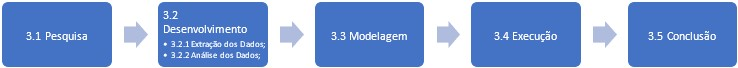
\includegraphics[width=15cm]{images/RF_img/FluxoMetodologia.jpg}
	\end{center}
	\fdadospesquisa
\end{figure}

\subsection[Pesquisa]{Pesquisa}
\label{Pesquisa}
Esta etapa se trata da pesquisa por mais projetos desenvolvidos no assunto abordado, pela revisão bibliográfica de mais artigos e exemplos de sucesso no desenvolvimento e escrita/documentação do que foi estudado.

Esta etapa se trata da pesquisa por mais projetos desenvolvidos no assunto abordado, pela revisão bibliográfica de mais artigos e exemplos de sucesso no desenvolvimento e escrita/documentação do que foi estudado.

\subsection[Desenvolvimento]{Desenvolvimento}
\label{Desenvolvimento}

Para o desenvolvimento do estudo, devido a capacidade computacional, as análises foram reduzidas para o estado de SP como validação do modelo.

\subsubsection[Extração dos Dados]{Extração dos Dados}
\label{Extração dos Dados}

Nesta etapa, foram coletados dados de estados, regiões, regiões imediatas, municípios, latitude, longitude e população por município diretamente da \sigla{API}{Interface de Programação de Aplicativos} do \sigla{IBGE}{Instituto Brasileiro de Geografia e Estatística} \cite{ibge:2025:divisoesregionais} (\autoref{tab:dados_municipios}).

\begin{table}[h!]
\centering
\caption{Características das Colunas de Dados dos Municípios Brasileiros}
\label{tab:dados_municipios}
\begin{tabular}{|p{5cm}|p{2cm}|p{2cm}|p{5cm}|} % Ajuste das larguras das colunas
\hline
\textbf{Coluna} & \textbf{Número de Linhas} & \textbf{Tipo} & \textbf{Descrição} \\
\hline
uf & 645 & object & Sigla do estado \\
\hline % Linha adicionada
regiao & 645 & object & Região do Brasil \\
\hline % Linha adicionada
codigo\_ibge & 645 & object & Código único do município \\
\hline % Linha adicionada
nome\_cidade & 645 & object & Nome da cidade \\
\hline % Linha adicionada
latitude\_cidade & 645 & float64 & Latitude da cidade \\
\hline % Linha adicionada
longitude\_cidade & 645 & float64 & Longitude da cidade \\
\hline % Linha adicionada
Nome do Município & 645 & object & Nome da cidade \\
\hline % Linha adicionada
Nome da Região Imediata & 645 & object & Nome da região geográfica imediata \\
\hline % Linha adicionada
Nome do Município da Região Imediata & 645 & object & Nome do principal município da região geográfica imediata \\
\hline % Linha adicionada
Pop\_2022 & 645 & float64 & População estimada para 2022 \\
\hline
\end{tabular}
\end{table}

\subsubsection[Geração de Dados e Definições de Parâmetros]{Geração de Dados e Definições de Parâmetros}
\label{Geração de Dados}\par

Foram gerados os dados de parâmetro, que foram apresentados na seção \ref{Modelagem Matemática}, para que as instâncias sejam testadas. Seguindo a mesma organização da seção apresentada, os dados são separados por clientes, postos avançados, CD e fábrica, com seus respectivos valores por instâncias.

\paragraph[Clientes ZDs]{Clientes ZDs}
\label{Clientes}

Os parâmetros para clientes basicamente são dois: demanda de instalação e demanda de desinstalação \autoref{tab:clientes}. Os dados de demanda estão por latitude e longitude, sendo dados gerados através dos dados de população, que foi extraída conforme na seção \ref{Extração dos Dados}.\par

\begin{table}[h!]
\centering
\caption{clientes}
\label{tab:clientes}
\begin{tabular}{|c|c|c|c|}
\hline
\textbf{Variável} & \textbf{Instância 1} & \textbf{Instância 2} & \textbf{Instância 3} \\
\hline
$dem^{rj}_{j,t}$ & $dem^{rj}_{j,t} \in [0, 1.146M]$ & $dem^{rj}_{j,t} \in [0, 1.172M]$ & $dem^{rj}_{j,t} \in [0, 1.179M]$ \\
\hline
$dem^{aj}_{j,t}$ & $dem^{aj}_{j,t} \in [0, 1.322M]$ & $dem^{aj}_{j,t} \in [0, 1.362M]$ & $dem^{aj}_{j,t} \in [0, 1.367M]$ \\
\hline
\end{tabular}
\end{table}

Inicialmente foi gerado um histograma para classificar os municípios conforme sua população, utilizando a faixa de 50 mil habitantes como critério principal. A visualização dessa classificação pode ser encontrada na Figura \ref{fig_hist_c_sp}.

\begin{figure}[htb]
	\caption{\label{fig_hist_c_sp} Histograma da população do estado de São Paulo}
	\begin{center}
            \includegraphics[width=10cm]{images/RF_img/Pop_c_SP_Hist.png}
	\end{center}
	\fdadospesquisa
\end{figure}

O estado de São Paulo possui uma concentração muito grande e discrepante na capital em relação às outras cidades, tendo sua faixa populacional acima de 12 milhões de habitantes. Com isso, foi necessário um tratamento à parte, sendo criado um novo histograma sem a cidade de São Paulo, utilizando faixa populacional de 25 mil habitantes \autoref{fig_hist_s_sp}.

\begin{figure}[htb]
	\caption{\label{fig_hist_s_sp} Histograma da população do estado de São Paulo sem a capital}
	\begin{center}
            \includegraphics[width=10cm]{images/RF_img/Pop_s_SP_Hist.png}
	\end{center}
	\fdadospesquisa
\end{figure}

A geração da demanda foi realizada através da demanda total de maquinetas, que foi de 20 milhões em um ano; em seguida, a empresa que está sendo analisada possui um \emph{market share} (percentual de participação do mercado) de 30\%, com isso foi aplicado este percentual definindo a demanda anual da empresa em questão. Calcula-se a média mensal e aplica-se uma variação randômica seguindo uma distribuição normal com variação de 10\%.

A demanda considerada foi limitada ao estado de SP devido a restrições computacionais, totalizando cerca de 1,3 milhão de instalações anuais, com média de 110 mil por mês. Em função da LR da cadeia, a demanda de desinstalação é estimada em 80\% da demanda de instalação. A Figura \ref{grafico_demanda_isnt_desinst_01} apresenta as curvas de demanda anual (instalação e desinstalação) para a instância 1.

\begin{figure}[htb]
	\caption{\label{grafico_demanda_isnt_desinst_01} Gráfico de Demanda de Instalação e Desinstalação para o Estado de São Paulo - Instância 1}
	\begin{center}
            \includegraphics[width=10cm]{images/RF_img/Demanda_linha_inst_01.png}
	\end{center}
	\fdadospesquisa
\end{figure}

A Instância 2 simula a sazonalidade de Natal, aplicando um acréscimo de 20\% na demanda de instalação em dezembro. Em função da LR e do volume instalado, a demanda de desinstalação apresenta um aumento correspondente de 20\% em janeiro. O perfil da demanda desta instância está detalhado na Figura \ref{grafico_demanda_isnt_desinst_02}.

\begin{figure}[htb]
	\caption{\label{grafico_demanda_isnt_desinst_02} Gráfico de Demanda de Instalação e Desinstalação para o Estado de São Paulo - Instância 2}
	\begin{center}
            \includegraphics[width=10cm]{images/RF_img/Demanda_linha_inst_02.png}
	\end{center}
	\fdadospesquisa
\end{figure}

Para a instância 3, é aplicado uma sazonalidade para o período de carnaval, ocorrendo um aumento de 20\% na instalação no mês de fevereiro e o mesmo aumento de 20\% na desinstalação de março, em decorrência do aumento ocorrido na instalação no mês anterior (\autoref{grafico_demanda_isnt_desinst_03}).

\begin{figure}[htb]
	\caption{\label{grafico_demanda_isnt_desinst_03} Gráfico de Demanda de Instalação e Desinstalação para o Estado de São Paulo - Instância 3}
	\begin{center}
            \includegraphics[width=10cm]{images/RF_img/Demanda_linha_inst_03.png}
	\end{center}
	\fdadospesquisa
\end{figure}

As demandas foram contabilizadas por cidade, porém para melhorar o processamento computacional, a demanda foi consolidada em ZDs. Para definir essas zonas, foram selecionadas 50\% das cidades com maior demanda e com isso a demanda restante foi redistribuída entre estas cidades proporcionalmente. Com isso houve uma redução em 50\% da base de dados total.

% Desta maneira, a distribuição das ZDs por faixa de demanda é apresentada conforme \autoref{hist_faixa_cidade_01}, percebe-se que 5 ZDs possuem o volume muito alto, enquanto as demais são mais uniformemente distribuídas para a instância 1 e .

% \begin{figure}[htb]
% 	\caption{\label{hist_faixa_cidade_01} Histograma de Cidades por Faixa Demanda }
% 	\begin{center}
%             \includegraphics[width=10cm]{images/RF_img/Faixa_Dem_Cidades_inst_01.png}
% 	\end{center}
% 	\fdadospesquisa
% \end{figure}\par

% \begin{figure}[htb]
% 	\caption{\label{hist_faixa_cidade_02} Histograma de Cidades por Faixa Demanda }
% 	\begin{center}
%             \includegraphics[width=10cm]{images/RF_img/Faixa_Dem_Cidades_inst_02.png}
% 	\end{center}
% 	\fdadospesquisa
% \end{figure}\par

% \begin{figure}[htb]
% 	\caption{\label{hist_faixa_cidade_03} Histograma de Cidades por Faixa Demanda }
% 	\begin{center}
%             \includegraphics[width=10cm]{images/RF_img/Faixa_Dem_Cidades_inst_03.png}
% 	\end{center}
% 	\fdadospesquisa
% \end{figure}\par



\paragraph[Postos Avançados (PAs)]{Postos Avançados (PAs)}
\label{Postos Avançados}

Para os Pontos de Atendimento (PAs), foram identificadas algumas cidades com potencial para implantação, com base nas Regiões Geográficas Imediatas. De acordo com o \citeonline{ibge:2024:compreendendoterritorio}, essas regiões representam áreas cujos habitantes recorrem a centros urbanos próximos para suprir necessidades imediatas, como acesso a emprego, saúde, educação, consumo e serviços públicos. Dentro de cada região imediata, foram selecionadas as duas maiores cidades, obtendo-se um total de 112 cidades conforme apresentado na \autoref{poss_pa_sp}.

\begin{figure}[htb]
	\caption{\label{poss_pa_sp} Mapa com as possíveis cidades para abertura de um PA.}
	\begin{center}
            \includegraphics[width=10cm]{images/RF_img/poss_pa_sp.png}
	\end{center}
	\fdadospesquisa
\end{figure}

Para as instâncias 1,2 e 3, o parâmetro $n^{p}$ (quantidade máxima de aberturas de PAs) foi definido como 70\% do total de cidades elegíveis à instalação de um PA. O parâmetro $e^{p}_{p,t}$ (limite máximo de máquinas em estoque) foi determinado individualmente para cada possível PA, com base na faixa de demanda da respectiva região imediata, sendo fixado em 125\% do valor da faixa de maior demanda. Esse critério visa garantir um estoque suficiente para cobrir até 36 dias de operação do PA.

Os parâmetros $m^{rp}_{p}$ (capacidade máxima de recebimento no PA) e $m^{ap}_{p}$ (capacidade máxima de envio do PA) foram estipulados como aproximadamente 80\% do estoque inicial, assegurando o atendimento da demanda estimada para um período de 30 dias. O parâmetro $c^{pj}_{p,j}$ (indicador de pertencimento regional entre os PAs e as ZDs) assume sempre o valor 1, uma vez que o modelo foi restrito ao estado de São Paulo; portanto, todas as ZDs pertencem ao mesmo estado onde os PAs podem ser implantados.

O cálculo do parâmetro de distância $d^{pj}_{p,j}$, entre os PAs e as ZDs, é realizado utilizando-se a \textbf{distância euclidiana}, a partir das coordenadas geográficas (latitude e longitude) dos respectivos pontos, conforme especificado na \autoref{tab:parametros_pa}.

Esta opção metodológica se justifica pela indisponibilidade de uma base de dados fidedigna que contenha as distâncias rodoviárias reais entre os municípios do estado de São Paulo. É importante ressaltar que a utilização da distância euclidiana implica uma simplificação do problema, não incorporando fatores do mundo real, como rotas específicas ou cobranças por pedágio.

\begin{table}[h!]
\centering
\caption{Parâmetros PA}
\label{tab:parametros_pa}
\begin{tabular}{|c|c|c|c|}
\hline
\textbf{Variável} & \textbf{Instância 1, 2 e 3} \\
\hline
$n^{p}$ & 112 \\
\hline
$e^{p}_{p,t}$ & $e^{p}_{p,t} \in [550, 176.300]$ \\
\hline
$m^{rp}_{p}$ & $m^{rp}_{p} \in [275, 88.150]$ \\
\hline
$m^{ap}_{p}$ & $m^{ap}_{p} \in [275, 88.150]$ \\
\hline
$c^{pj}_{p,j}$ & 1 \\
\hline
$d^{pj}_{p,j}$ & $d^{pj}_{p,j} \in [0, 830]$ \\
\hline
\end{tabular}
\end{table}

\paragraph[CDs]{CDs}
\label{CD}

A seleção das cidades para a possível instalação de CDs considerou diversos critérios estratégicos: proximidade com aeroportos, infraestrutura adequada para operações logísticas, reconhecimento histórico como polos logísticos, além da localização próxima à fábrica e à empresa responsável pelos descartes. As cidades escolhidas foram: Americana, Guarulhos, Hortolândia, Jundiaí, Mogi das Cruzes, Osasco, São José dos Campos, Sorocaba e Suzano (\autoref{poss_cd_sp}).

\begin{figure}[htb]
	\caption{\label{poss_cd_sp} Mapa com as possíveis cidades para abertura de um PA.}
	\begin{center}
            \includegraphics[width=10cm]{images/RF_img/poss_cd_sp.png}
	\end{center}
	\fdadospesquisa
\end{figure}

Para a instância 1, o parâmetro $n^{c}$ (quantidade máxima de aberturas de CDs) foi definido como 1. O parâmetro $e^{c}_{i,t}$ (limite máximo de máquinas em estoque) é calculado com um acréscimo de 20\% sobre o estoque inicial de 200 mil máquinas — sendo 100 mil aptas para uso e 100 mil destinadas ao descarte ou reparo na fábrica. Esse valor de 100 mil foi estabelecido com o objetivo de garantir atendimento à demanda por um período de 30 dias.

Os parâmetros $m^{rc}{i}$ (limite máximo de recebimento de máquinas no CD) e $m^{ac}{i}$ (limite máximo de envio de máquinas pelo CD) são definidos com base nas capacidades operacionais esperadas do centro.

O parâmetro $c^{cp}_{i,p}$, que funciona como um indicador binário de pertencimento regional entre os CDs e os PAs, é fixado em 1, dada a premissa de que todas as instalações estão localizadas na mesma unidade federativa.

As distâncias $d^{cd}_{i,d}$ (entre os CDs e os pontos de descarte) e $d^{cp}_{i,p}$ (entre os CDs e os PAs) são calculadas utilizando-se a \textit{distância euclidiana}, a partir de suas coordenadas geográficas (latitude e longitude).

Por fim, o parâmetro $r^{c}$, que representa o fator de reenvio (ou proporção) para os CDs das máquinas recebidas dos PAs, é definido como $0,7$.  

\begin{table}[h!]
\centering
\caption{Parâmetros do CD}
\label{tab:parametros_cd}
\begin{tabular}{|c|c|c|c|}
\hline
\textbf{Variável} & \textbf{Instância 1, 2 e 3} \\
\hline
$n^{c}$ & 1, 2 e 3 \\
\hline
$e^{c}_{i,t}$ & 230.000 \\
\hline
$m^{rc}_{i}$ & 82.500 \\
\hline
$m^{ac}_{i}$ & 82.500 \\
\hline
$c^{cp}_{i,p}$ & 1 \\
\hline
$d^{cd}_{i,d}$ & $d^{cd}_{i,d} \in [0, 659]$ \\
\hline
$d^{cp}_{i,p}$ & $d^{cp}_{i,p} \in [4, 109]$ \\
\hline
$r^{c}$ & 0,7 \\
\hline
\end{tabular}
\end{table}

\paragraph[Fábrica]{Fábrica}
\label{Fábrica}

Os parâmetros empregados na configuração das Instâncias 1, 2 e 3 são idênticos, uma vez que foram obtidos a partir do histórico operacional fornecido pela empresa. Entretanto, a análise dos dados revela que a capacidade de envio e recebimento atribuída à fábrica é proporcionalmente inferior quando comparada aos demais pontos de estoque. Essa diferença se justifica pela função primária da fábrica, que é focada na produção e reparo das maquinas, e não na gestão de grandes volumes logísticos de distribuição.

\begin{table}[h!]
\centering
\caption{Parâmetros do Fabricante}
\label{tab:parametros_fabricante}
\begin{tabular}{|c|c|c|c|}
\hline
\textbf{Variável} & \textbf{Instâncias 1, 2 e 3} \\
\hline
$m^{rf}_{l}$ & 11.700 \\
\hline
$m^{af}_{l}$ & 11.700 \\
\hline
$e^{f}_{l,t}$ & 62.404 \\
\hline
$c^{fc}_{l,i}$ & $c^{fc}_{l,i} \in [0, 1]$ \\
\hline
$d^{fc}_{l,i}$ & $d^{fc}_{l,i} \in [5, 102]$ \\
\hline
$r^{f}$ & 0,2 \\
\hline
\end{tabular}
\end{table}


\chapter{Experimentos Computacionais}
\label{chapter:exp_comp}

\section{Geração dos Dados}\label{Metodologia.}

O projeto proposto será composto pelas etapas que seguem (\autoref{fig_fluxo_met}), sendo que neste capítulo, trata-se da geração de dados e execução. Foram geradas três instâncias para a análise da rede logística. 

\begin{figure}[htb]
	\caption{\label{fig_fluxo_met} Fluxo logístico do envio e retorno de maquinetas, laço fechado}
	\begin{center}
            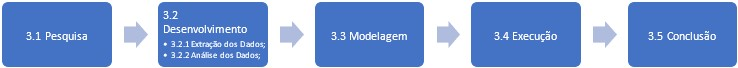
\includegraphics[width=15cm]{images/RF_img/FluxoMetodologia.jpg}
	\end{center}
	\fdadospesquisa
\end{figure}


 


A implementação detalhada do código-fonte está disponível no Apêndice \ref{anexo:codigo}, através de um link para o github.


%\subsection[Pesquisa]{Pesquisa}
%\label{Pesquisa}
%Esta etapa se trata da pesquisa por mais projetos desenvolvidos no assunto abordado, pela revisão bibliográfica de mais artigos e exemplos de sucesso no desenvolvimento e escrita/documentação do que foi estudado.

%Esta etapa se trata da pesquisa por mais projetos desenvolvidos no assunto abordado, pela revisão bibliográfica de mais artigos e exemplos de sucesso no desenvolvimento e escrita/documentação do que foi estudado.

%\subsection[Desenvolvimento]{Desenvolvimento}
%\label{Desenvolvimento}

%Para o desenvolvimento do estudo, devido a capacidade computacional, as análises foram reduzidas para o estado de SP como validação do modelo.

\subsection{Geração de Dados e Definições de Parâmetros}
\label{Extração dos Dados}

Nesta etapa, foram coletados dados de estados, regiões, regiões imediatas, municípios, latitude, longitude e população por município diretamente da \sigla{API}{Interface de Programação de Aplicativos} do \sigla{IBGE}{Instituto Brasileiro de Geografia e Estatística} \cite{ibge:2025:divisoesregionais} (\autoref{tab:dados_municipios}).

\begin{table}[h!]
\centering
\caption{Características das Colunas de Dados dos Municípios Brasileiros}
\label{tab:dados_municipios}
\begin{tabular}{|p{5cm}|p{2cm}|p{2cm}|p{5cm}|} % Ajuste das larguras das colunas
\hline
\textbf{Coluna} & \textbf{Número de Linhas} & \textbf{Tipo} & \textbf{Descrição} \\
\hline
uf & 645 & object & Sigla do estado \\
\hline % Linha adicionada
regiao & 645 & object & Região do Brasil \\
\hline % Linha adicionada
codigo\_ibge & 645 & object & Código único do município \\
\hline % Linha adicionada
nome\_cidade & 645 & object & Nome da cidade \\
\hline % Linha adicionada
latitude\_cidade & 645 & float64 & Latitude da cidade \\
\hline % Linha adicionada
longitude\_cidade & 645 & float64 & Longitude da cidade \\
\hline % Linha adicionada
Nome do Município & 645 & object & Nome da cidade \\
\hline % Linha adicionada
Nome da Região Imediata & 645 & object & Nome da região geográfica imediata \\
\hline % Linha adicionada
Nome do Município da Região Imediata & 645 & object & Nome do principal município da região geográfica imediata \\
\hline % Linha adicionada
Pop\_2022 & 645 & float64 & População estimada para 2022 \\
\hline
\end{tabular}
\end{table}

%\subsubsection[Geração de Dados e Definições de Parâmetros]{Geração de Dados e Definições de Parâmetros}
%\label{Geração de Dados}\par

Para o teste das instâncias, foram gerados os parâmetros correspondentes ao modelo apresentado na Seção \ref{Modelagem Matemática}. Seguindo a estrutura metodológica, os dados de entrada encontram-se segmentados por clientes, PAs, CDs e fábrica. Como elemento central para a minimização da função objetivo, destacam-se os parâmetros financeiros associados aos custos fixos de abertura e manutenção das facilidades logísticas, bem como o custo de transporte por máquina e por quilômetro rodado, conforme sumarizado na \autoref{tab:parametros_custos}.

\begin{table}[h!]
\centering
\caption{Parâmetros de custos do sistema logístico}
\label{tab:parametros_custos}
\begin{tabular}{|c|l|c|}
\hline
\textbf{Símbolo} & \textbf{Descrição} & \textbf{Valor (R\$)} \\
\hline
$h_{i}$ & Custo de abertura de Centro de Distribuição (CD) & 3.000.000 \\
\hline
$v_{i}$ & Custo anual de manutenção de Centro de Distribuição (CD) & 100.000 \\
\hline
$u_{p}$ & Custo de abertura de Posto Avançado (PA) & [3.000, 864.000]* \\
\hline
$x_{p}$ & Custo anual de manutenção de Posto Avançado (PA) & [150, 43.200]* \\
\hline
$k$ & Custo de transporte por quilômetro por unidade & 0,015 \\
\hline
\end{tabular}
\end{table}

\subsubsection{Clientes - Zonas de Demanda (ZDs)}
\label{Clientes}

Os parâmetros para clientes basicamente são dois: demanda de instalação e demanda de desinstalação \autoref{tab:clientes}. Os dados de demanda estão por latitude e longitude, sendo dados gerados através dos dados de população, que foi extraída conforme na seção \ref{Extração dos Dados}.\par

\begin{table}[h!]
\centering
\caption{Clientes}
\label{tab:clientes}
\begin{tabular}{|c|c|c|c|}
\hline
\textbf{Variável} & \textbf{Instância 1} & \textbf{Instância 2} & \textbf{Instância 3} \\
\hline
$dem^{rj}_{j,t}$ & $dem^{rj}_{j,t} \in [0, 1.146M]$ & $dem^{rj}_{j,t} \in [0, 1.172M]$ & $dem^{rj}_{j,t} \in [0, 1.179M]$ \\
\hline
$dem^{aj}_{j,t}$ & $dem^{aj}_{j,t} \in [0, 1.322M]$ & $dem^{aj}_{j,t} \in [0, 1.362M]$ & $dem^{aj}_{j,t} \in [0, 1.367M]$ \\
\hline
\end{tabular}
\end{table}

Inicialmente foi gerado um histograma para classificar os municípios conforme sua população, utilizando a faixa de 50 mil habitantes como critério principal. A visualização dessa classificação pode ser encontrada na Figura \ref{fig_hist_c_sp}.

\begin{figure}[htb]
	\caption{\label{fig_hist_c_sp} Histograma da população do estado de São Paulo}
	\begin{center}
            \includegraphics[width=10cm]{images/RF_img/Pop_c_SP_Hist.png}
	\end{center}
	\fdadospesquisa
\end{figure}

O estado de São Paulo possui uma concentração muito grande e discrepante na capital em relação às outras cidades, tendo sua faixa populacional acima de 12 milhões de habitantes. Com isso, foi necessário um tratamento à parte, sendo criado um novo histograma sem a cidade de São Paulo, utilizando faixa populacional de 25 mil habitantes \autoref{fig_hist_s_sp}.

\begin{figure}[htb]
	\caption{\label{fig_hist_s_sp} Histograma da população do estado de São Paulo sem a capital}
	\begin{center}
            \includegraphics[width=10cm]{images/RF_img/Pop_s_SP_Hist.png}
	\end{center}
	\fdadospesquisa
\end{figure}

A geração da demanda foi realizada através da demanda total de maquinetas, que foi de 20 milhões em um ano; em seguida, a empresa que está sendo analisada possui um \emph{market share} (percentual de participação do mercado) de 30\%, com isso foi aplicado este percentual definindo a demanda anual da empresa em questão. Calcula-se a média mensal e aplica-se uma variação randômica seguindo uma distribuição normal com variação de 10\%.

A demanda considerada foi limitada ao estado de SP devido a restrições computacionais, totalizando cerca de 1,3 milhão de instalações anuais, com média de 110 mil por mês. Em função da LR da cadeia, a demanda de desinstalação é estimada em 80\% da demanda de instalação. A Figura \ref{grafico_demanda_isnt_desinst_01} apresenta as curvas de demanda anual (instalação e desinstalação) para a instância 1.

\begin{figure}[htb]
	\caption{\label{grafico_demanda_isnt_desinst_01} Gráfico de Demanda de Instalação e Desinstalação para o Estado de São Paulo - Instância 1}
	\begin{center}
            \includegraphics[width=10cm]{images/RF_img/Demanda_linha_inst_01.png}
	\end{center}
	\fdadospesquisa
\end{figure}

A Instância 2 simula a sazonalidade de Natal, aplicando um acréscimo de 20\% na demanda de instalação em dezembro. Em função da LR e do volume instalado, a demanda de desinstalação apresenta um aumento correspondente de 20\% em janeiro. O perfil da demanda desta instância está detalhado na Figura \ref{grafico_demanda_isnt_desinst_02}.

\begin{figure}[htb]
	\caption{\label{grafico_demanda_isnt_desinst_02} Gráfico de Demanda de Instalação e Desinstalação para o Estado de São Paulo - Instância 2}
	\begin{center}
            \includegraphics[width=10cm]{images/RF_img/Demanda_linha_inst_02.png}
	\end{center}
	\fdadospesquisa
\end{figure}

Para a instância 3, é aplicado uma sazonalidade para o período de carnaval, ocorrendo um aumento de 20\% na instalação no mês de fevereiro e o mesmo aumento de 20\% na desinstalação de março, em decorrência do aumento ocorrido na instalação no mês anterior (\autoref{grafico_demanda_isnt_desinst_03}).

\begin{figure}[htb]
	\caption{\label{grafico_demanda_isnt_desinst_03} Gráfico de Demanda de Instalação e Desinstalação para o Estado de São Paulo - Instância 3}
	\begin{center}
            \includegraphics[width=10cm]{images/RF_img/Demanda_linha_inst_03.png}
	\end{center}
	\fdadospesquisa
\end{figure}

As demandas foram contabilizadas por cidade, porém para melhorar o processamento computacional, a demanda foi consolidada em ZDs. Para definir essas zonas, foram selecionadas 50\% das cidades com maior demanda e com isso a demanda restante foi redistribuída entre estas cidades proporcionalmente. Com isso houve uma redução em 50\% da base de dados total.

% Desta maneira, a distribuição das ZDs por faixa de demanda é apresentada conforme \autoref{hist_faixa_cidade_01}, percebe-se que 5 ZDs possuem o volume muito alto, enquanto as demais são mais uniformemente distribuídas para a instância 1 e .

% \begin{figure}[htb]
% 	\caption{\label{hist_faixa_cidade_01} Histograma de Cidades por Faixa Demanda }
% 	\begin{center}
%             \includegraphics[width=10cm]{images/RF_img/Faixa_Dem_Cidades_inst_01.png}
% 	\end{center}
% 	\fdadospesquisa
% \end{figure}\par

% \begin{figure}[htb]
% 	\caption{\label{hist_faixa_cidade_02} Histograma de Cidades por Faixa Demanda }
% 	\begin{center}
%             \includegraphics[width=10cm]{images/RF_img/Faixa_Dem_Cidades_inst_02.png}
% 	\end{center}
% 	\fdadospesquisa
% \end{figure}\par

% \begin{figure}[htb]
% 	\caption{\label{hist_faixa_cidade_03} Histograma de Cidades por Faixa Demanda }
% 	\begin{center}
%             \includegraphics[width=10cm]{images/RF_img/Faixa_Dem_Cidades_inst_03.png}
% 	\end{center}
% 	\fdadospesquisa
% \end{figure}\par



\subsubsection{Postos Avançados (PAs)}
\label{Postos Avançados}

Para os PAs, foram identificadas algumas cidades com potencial para implantação, com base nas Regiões Geográficas Imediatas. De acordo com o \citeonline{ibge:2024:compreendendoterritorio}, essas regiões representam áreas cujos habitantes recorrem a centros urbanos próximos para suprir necessidades imediatas, como acesso a emprego, saúde, educação, consumo e serviços públicos. Dentro de cada região imediata, foram selecionadas as duas maiores cidades, obtendo-se um total de 112 cidades conforme apresentado na \autoref{poss_pa_sp}.

\begin{figure}[htb]
	\caption{\label{poss_pa_sp} Mapa com as possíveis cidades para abertura de um PA.}
	\begin{center}
            \includegraphics[width=10cm]{images/RF_img/poss_pa_sp.png}
	\end{center}
	\fdadospesquisa
\end{figure}

Para as instâncias 1,2 e 3, o parâmetro $n^{p}$ (quantidade máxima de aberturas de PAs) foi definido como 70\% do total de cidades elegíveis à instalação de um PA. O parâmetro $e^{p}_{p,t}$ (limite máximo de máquinas em estoque) foi determinado individualmente para cada possível PA, com base na faixa de demanda da respectiva região imediata, sendo fixado em 125\% do valor da faixa de maior demanda. Esse critério visa garantir um estoque suficiente para cobrir até 36 dias de operação do PA.

Os parâmetros $m^{rp}_{p}$ (capacidade máxima de recebimento no PA) e $m^{ap}_{p}$ (capacidade máxima de envio do PA) foram estipulados como aproximadamente 80\% do estoque inicial, assegurando o atendimento da demanda estimada para um período de 30 dias. O parâmetro $c^{pj}_{p,j}$ (indicador de pertencimento regional entre os PAs e as ZDs) assume sempre o valor 1, uma vez que o modelo foi restrito ao estado de São Paulo; portanto, todas as ZDs pertencem ao mesmo estado onde os PAs podem ser implantados.

O cálculo do parâmetro de distância $d^{pj}_{p,j}$ (entre os PAs e as ZDs) é realizado utilizando-se a \textbf{distância euclidiana}, a partir das coordenadas geográficas (latitude e longitude) dos respectivos pontos, conforme especificado na \autoref{tab:parametros_pa}.

Esta opção metodológica se justifica pela indisponibilidade de uma base de dados fidedigna que contenha as distâncias rodoviárias reais entre os municípios do estado de São Paulo. É importante ressaltar que a utilização da distância euclidiana implica uma simplificação do problema, não incorporando fatores do mundo real, como rotas específicas ou cobranças por pedágio.

\begin{table}[h!]
\centering
\caption{Parâmetros PA}
\label{tab:parametros_pa}
\begin{tabular}{|c|c|}
\hline
\textbf{Parâmetro} & \textbf{Instância 1, 2 e 3} \\
\hline
$n^{p}$ & 112 \\
\hline
$e^{p}_{p,t}$ & $e^{p}_{p,t} \in [550, 176.300]$ \\
\hline
$m^{rp}_{p}$ & $m^{rp}_{p} \in [275, 88.150]$ \\
\hline
$m^{ap}_{p}$ & $m^{ap}_{p} \in [275, 88.150]$ \\
\hline
$c^{pj}_{p,j}$ & 1 \\
\hline
$d^{pj}_{p,j}$ & $d^{pj}_{p,j} \in [0, 830]$ \\
\hline
\end{tabular}
\end{table}

\subsubsection{Centros de Distribuição (CDs)}
\label{Centros de Distribuição}

A seleção das cidades para a possível instalação de Centros de Distribuição (CDs) considerou diversos critérios estratégicos: proximidade com aeroportos, infraestrutura adequada para operações logísticas, reconhecimento histórico como polos logísticos, além da localização próxima à fábrica e à empresa responsável pelos descartes. As cidades escolhidas foram: Americana, Guarulhos, Hortolândia, Jundiaí, Mogi das Cruzes, Osasco, São José dos Campos, Sorocaba e Suzano (\autoref{poss_cd_sp}).

\begin{figure}[htb]
	\caption{\label{poss_cd_sp} Mapa com as possíveis cidades para abertura de um PA.}
	\begin{center}
            \includegraphics[width=10cm]{images/RF_img/poss_cd_sp.png}
	\end{center}
	\fdadospesquisa
\end{figure}

O parâmetro $e^{c}_{i,t}$ (limite máximo de máquinas em estoque) é calculado com um acréscimo de 20\% sobre o estoque inicial de 200 mil máquinas — sendo 100 mil aptas para uso e 100 mil destinadas ao descarte ou reparo na fábrica. Esse valor de 100 mil foi estabelecido com o objetivo de garantir atendimento à demanda por um período de 30 dias.

Os parâmetros $m^{rc}{i}$ (limite máximo de recebimento de máquinas no CD) e $m^{ac}{i}$ (limite máximo de envio de máquinas pelo CD) são definidos com base nas capacidades operacionais esperadas do centro.

O parâmetro $c^{cp}_{i,p}$, que funciona como um indicador binário de pertencimento regional entre os CDs e os PAs, é fixado em 1, dada a premissa de que todas as instalações estão localizadas na mesma unidade federativa.

As distâncias $d^{cd}_{i,d}$ (entre os CDs e os pontos de descarte) e $d^{cp}_{i,p}$ (entre os CDs e os PAs) são calculadas utilizando-se a \emph{distância euclidiana}, a partir de suas coordenadas geográficas (latitude e longitude).

Por fim, o parâmetro $r^{c}$, que representa o fator de reenvio (ou proporção) para os CDs das máquinas recebidas dos PAs, é definido como $0,7$.  

\begin{table}[h!]
\centering
\caption{Parâmetros do CD}
\label{tab:parametros_cd}
\begin{tabular}{|c|c|}
\hline
\textbf{Variável} & \textbf{Instância 1, 2 e 3} \\
\hline
$n^{c}$ & 1, 2 e 3 \\
\hline
$e^{c}_{i,t}$ & 230.000 \\
\hline
$m^{rc}_{i}$ & 82.500 \\
\hline
$m^{ac}_{i}$ & 82.500 \\
\hline
$c^{cp}_{i,p}$ & 1 \\
\hline
$d^{cd}_{i,d}$ & $d^{cd}_{i,d} \in [0, 659]$ \\
\hline
$d^{cp}_{i,p}$ & $d^{cp}_{i,p} \in [4, 109]$ \\
\hline
$r^{c}$ & 0,7 \\
\hline
\end{tabular}
\end{table}

\subsubsection{Fábrica}
\label{Fábrica}

Os parâmetros empregados na configuração das Instâncias 1, 2 e 3 são idênticos, uma vez que foram obtidos a partir do histórico operacional fornecido pela empresa. Entretanto, a análise dos dados revela que a capacidade de envio e recebimento atribuída à fábrica é proporcionalmente inferior quando comparada aos demais pontos de estoque. Essa diferença se justifica pela função primária da fábrica, que é focada na produção e reparo das maquinas, e não na gestão de grandes volumes logísticos de distribuição.

\begin{table}[h!]
\centering
\caption{Parâmetros do Fabricante}
\label{tab:parametros_fabricante}
\begin{tabular}{|c|c|}
\hline
\textbf{Parâmetro} & \textbf{Instâncias 1, 2 e 3} \\
\hline
$m^{rf}_{l}$ & 11.700 \\
\hline
$m^{af}_{l}$ & 11.700 \\
\hline
$e^{f}_{l,t}$ & 62.404 \\
\hline
$c^{fc}_{l,i}$ & $c^{fc}_{l,i} \in [0, 1]$ \\
\hline
$d^{fc}_{l,i}$ & $d^{fc}_{l,i} \in [5, 102]$ \\
\hline
$r^{f}$ & 0,2 \\
\hline
\end{tabular}
\end{table}



\subsection{Análise dos Dados}
\label{Análise dos Dados}

Analisando o mapa de calor, com as divisões das regiões imediatas do estado de SP, percebe-se que há uma concentração populacional em torno da capital, com isso a demanda também se concentra nesta região, além de nestas regiões os PAs serem maiores, pois para o atendimento da demanda em regiões que possuem maior demanda, o parâmetro indica PAs com capacidade maior de atendimento. \autoref{fig_mapa_pop_sp}. 

\begin{figure}[htb]
	\caption{\label{fig_mapa_pop_sp} Mapa de calor populacional do estado de São Paulo}
	\begin{center}
            \includegraphics[width=14cm]{images/RF_img/Mapa_Pop_SP.png}
	\end{center}
	\fdadospesquisa
\end{figure}

\section[Resultados da Otimização e Comparativo de Custos]{Resultados da Otimização e Comparativo de Custos}

O modelo de Programação Linear Inteira Mista (PLIM) proposto foi implementado utilizando a linguagem de programação \textbf{Python 3.11} e resolvido pelo \emph{solver} \textbf{Gurobi Optimizer} na \textbf{versão 12.0.2} (build \texttt{v12.0.2rc0}, \texttt{win64}), reconhecido por sua alta eficiência na resolução de problemas de grande escala.

\subsection{Ambiente Computacional e Configuração do \emph{Solver}}

Os experimentos computacionais foram realizados em um \emph{laptop} com sistema operacional \textbf{Windows 11} (versão 11.0), equipado com um processador \textbf{AMD Ryzen 7 5700U with Radeon Graphics} e arquitetura \texttt{[SSE2|AVX|AVX2]}. Para o processamento das instâncias, o \emph{solver} foi configurado para utilizar \textbf{4 \emph{threads}} de um total de 16 processadores lógicos (8 núcleos físicos) disponíveis.

A Tabela \ref{tab:parametros_gurobi} apresenta os principais parâmetros não-padrão configurados no \emph{solver} Gurobi para todas as execuções.

\begin{table}[htb]
    \centering
    \caption{Parâmetros Não-Padrão do Gurobi Optimizer}
    \label{tab:parametros_gurobi}
    \begin{tabular}{lcl}
        \toprule
        \textbf{Parâmetro} & \textbf{Valor} & \textbf{Descrição} \\
        \midrule
        \texttt{TimeLimit} & $\texttt{7200}$ & Tempo máximo de execução de 7200 segundos (2 horas). \\
        \texttt{MIPGap} & $\texttt{0.05}$ & Tolerância de \emph{gap} de otimalidade de 5\% (5.00e-02). \\
        \texttt{Threads} & $\texttt{4}$ & Número de \emph{threads} alocados. \\
        \texttt{Presolve} & $\texttt{2}$ & Nível agressivo de pré-processamento. \\
        \texttt{Method} & $\texttt{1}$ & Utilização do algoritmo \emph{Dual Simplex} para a fase linear. \\
        \texttt{NodefileStart} & $\texttt{5}$ & Início do armazenamento de nós em arquivo (padrão implícito de 5 GB). \\
        \bottomrule
    \end{tabular}
\end{table}

\subsection{Dimensão do Modelo e Desempenho Computacional}

O modelo de otimização resultante apresentou uma estrutura de grande porte, com dimensões médias consistentes em todas as instâncias: $2.571.077$ restrições (\emph{rows}), $1.298.196$ variáveis (\emph{columns}) e $8.099.220$ elementos não-nulos. Dentre as variáveis, $865.104$ são contínuas e $433.092$ são inteiras (binárias).

O pré-processamento (\emph{Presolve}) demonstrou eficácia, removendo consistentemente cerca de $44$ mil linhas e $21$ mil colunas do modelo antes da otimização.

Em todas as instâncias, o \emph{solver} Gurobi encontrou uma \textbf{solução factível e de boa qualidade dentro da tolerância} estabelecida pelo parâmetro \texttt{MIPGap}. A Tabela \ref{tab:desempenho_resumo} consolida os principais resultados de desempenho para o conjunto de instâncias:

\begin{table}[h!]
\centering
\caption{Resumo do desempenho computacional e convergência por instância}
\label{tab:desempenho_resumo}
\begin{tabular}{|c|c|c|c|}
\hline
\textbf{Variável} & \textbf{Instância 1} & \textbf{Instância 2} & \textbf{Instância 3} \\
\hline
Gap de Otimização (\%) & 4,5257\% & 4,7284\% & 4,6818\% \\
\hline
Tempo de Execução & 3.687,98s (1,02h) & 3.722,30s (1,03h) & 3.877,71s (1,08h) \\
\hline
\end{tabular}
\end{table}

Os resultados obtidos para o \emph{gap} de otimalidade (variando entre $4,5257\%$ e $4,7284\%$) confirmam que as soluções alcançadas estão dentro da margem de $5\%$ exigida. O tempo de execução, com um máximo de $3.877,71$ segundos (aproximadamente 1 hora e 4 minutos), demonstra a viabilidade computacional do modelo PLIM proposto para instâncias de grande porte, convergindo para soluções de alta qualidade em um tempo razoável, bem abaixo do limite de $7.200$ segundos.

\subsection{Análise por Instancia}

Na instância 1, foram abertos 79 PAs nas cidades de Adamantina, Americana, Andradina, Araçatuba, Araraquara, Assis, Avaré, Barra Bonita, Barretos, Bauru, Bebedouro, Birigui, Botucatu, Bragança Paulista, Campinas, Capão Bonito, Capivari, Catanduva, Cordeirópolis, Dracena, Franca, Garça, Guararapes, Guarulhos, Hortolândia, Indaiatuba, Itaí, Itajobi, Itapetininga, Itapeva, Itatiba, Itu, Jacareí, Jales, Jaú, Jundiaí, Junqueirópolis, Lençóis Paulista, Limeira, Lins, Lorena, Marília, Matão, Mirandópolis, Mirassol, Mogi Guaçu, Mogi Mirim, Osasco, Osvaldo Cruz, Ourinhos, Ouroeste, Palmeira d'Oeste, Paraguaçu Paulista, Pedregulho, Penápolis, Pindamonhangaba, Piracicaba, Pirassununga, Praia Grande, Presidente Prudente, Rancharia, Ribeirão Preto, Santa Cruz do Rio Pardo, Santo André, Santos, São Bernardo do Campo, São Carlos, São João da Boa Vista, São Joaquim da Barra, São José do Rio Preto, São José dos Campos, São Paulo, Sertãozinho, Sorocaba, Sumaré, Tupã, Ubatuba, Valentim Gentil, Vargem Grande do Sul. O CD foi aberto na cidade de Osasco (\autoref{fig_mapa_cd_pas_inst1}).

\begin{figure}[htb]
	\caption{\label{fig_mapa_cd_pas_inst1} Mapa da cidade de abertura do CD, cidades de abertura dos PAs e as cidades de PAs que não foram abertas - Instância 1}
	\begin{center}
            \includegraphics[width=14cm]{images/RF_img/CD_e_PAs_inst_1.png}
	\end{center}
	\fdadospesquisa
\end{figure}

\begin{figure}[htb]
	\caption{\label{fig_mapa_pas_zds_inst1} Mapa dos PAs que Atendem as ZDs - Instância 1}
	\begin{center}
            \includegraphics[width=14cm]{images/RF_img/PAs_ZDs_inst_1.png}
	\end{center}
	\fdadospesquisa
\end{figure}

Para a instância 2, foram abertos 88 PAs que pertencem as cidades de Adamantina, Americana, Andradina, Araçatuba, Araraquara, Assis, Atibaia, Barra Bonita, Barretos, Bastos, Bauru, Bebedouro, Birigui, Botucatu, Bragança Paulista, Campinas, Capão Bonito, Capivari, Caraguatatuba, Catanduva, Cordeirópolis, Dracena, Franca, Garça, Guararapes, Guaratinguetá, Guarulhos, Hortolândia, Iguape, Indaiatuba, Itaí, Itajobi, Itapetininga, Itapeva, Itatiba, Itu, Jacareí, Jales, Jaú, Jundiaí, Junqueirópolis, Lençóis Paulista, Limeira, Lins, Lorena, Marília, Matão, Mirandópolis, Mirassol, Mogi Guaçu, Mogi Mirim, Orlândia, Osasco, Osvaldo Cruz, Ourinhos, Ouroeste, Palmeira d'Oeste, Paraguaçu Paulista, Pedregulho, Penápolis, Pindamonhangaba, Piracicaba, Pirassununga, Praia Grande, Presidente Prudente, Promissão, Rancharia, Registro, Ribeirão Preto, Santa Cruz do Rio Pardo, Santo André, Santos, São Bernardo do Campo, São Carlos, São João da Boa Vista, São Joaquim da Barra, São José do Rio Preto, São José dos Campos, São Paulo, Sertãozinho, Sorocaba, Sumaré, Taubaté, Tupã, Ubatuba, Valentim Gentil, Vargem Grande do Sul, Votuporanga. O CD foi aberto em Osasco (\autoref{fig_mapa_cd_pas_inst2}).

\begin{figure}[htb]
	\caption{\label{fig_mapa_cd_pas_inst2} Mapa da cidade de abertura do CD, cidades de abertura dos PAs e as cidades de PAs que não foram abertas - Instância 2}
	\begin{center}
            \includegraphics[width=14cm]{images/RF_img/CD_e_PAs_inst_2.png}
	\end{center}
	\fdadospesquisa
\end{figure}

\begin{figure}[htb]
	\caption{\label{fig_mapa_pas_zds_inst2} Mapa dos PAs que Atendem as ZDs - Instância 2}
	\begin{center}
            \includegraphics[width=14cm]{images/RF_img/PAs_ZDs_inst_2.png}
	\end{center}
	\fdadospesquisa
\end{figure}

Na instância 03 foram abertos 78 PAs nas cidades de Adamantina, Americana, Andradina, Araçatuba, Araraquara, Assis, Avaré, Barra Bonita, Barretos, Bastos, Bauru, Bebedouro, Birigui, Botucatu, Bragança Paulista, Campinas, Capão Bonito, Capivari, Cordeirópolis, Franca, Garça, Guararapes, Guarulhos, Hortolândia, Indaiatuba, Itaí, Itajobi, Itapetininga, Itapeva, Itatiba, Itu, Jacareí, Jales, Jaú, Junqueirópolis, Lençóis Paulista, Lins, Lorena, Marília, Matão, Mirandópolis, Mirassol, Mogi Guaçu, Mogi Mirim, Orlândia, Osasco, Osvaldo Cruz, Ourinhos, Palmeira d'Oeste, Paraguaçu Paulista, Pedregulho, Penápolis, Pindamonhangaba, Piracicaba, Pirassununga, Praia Grande, Presidente Epitácio, Presidente Prudente, Presidente Venceslau, Promissão, Rancharia, Ribeirão Preto, Santa Cruz do Rio Pardo, Santo André, Santos, São Carlos, São João da Boa Vista, São Joaquim da Barra, São José do Rio Preto, São José dos Campos, São Paulo, Sertãozinho, Sorocaba, Sumaré, Tupã, Ubatuba, Valentim Gentil, Vargem Grande do Sul. O CD foi aberto na cidade de Guarulhos (\autoref{fig_mapa_cd_pas_inst3}).

\begin{figure}[htb]
	\caption{\label{fig_mapa_cd_pas_inst3} Mapa da cidade de abertura do CD, cidades de abertura dos PAs e as cidades de PAs que não foram abertas - Instância 3}
	\begin{center}
            \includegraphics[width=14cm]{images/RF_img/CD_e_PAs_inst_3.png}
	\end{center}
	\fdadospesquisa
\end{figure}

\begin{figure}[htb]
	\caption{\label{fig_mapa_pas_zds_inst3} Mapa dos PAs que Atendem as ZDs - Instância 3}
	\begin{center}
            \includegraphics[width=14cm]{images/RF_img/PAs_ZDs_inst_3.png}
	\end{center}
	\fdadospesquisa
\end{figure}

A decisão de abertura das facilidades PAs) prioriza regiões de alta demanda. Devido à maior capacidade instalada, estes PAs podem atender áreas mais distantes, eliminando a necessidade de novas implantações. Este padrão de decisão é justificado pelo fato de que o alto custo fixo de implantação de uma nova estrutura, no período analisado, supera o custo logístico operacional (movimentações). Essa relação custo-benefício é consistentemente observada nas três instâncias, conforme ilustrado nas Figuras \autoref{fig_mapa_pas_zds_inst1} (Instância 1), \autoref{fig_mapa_pas_zds_inst2} (Instância 2) e \autoref{fig_mapa_pas_zds_inst3} (Instância 3).

Em contrapartida, a Instância 2 apresenta uma particularidade: houve a abertura de dez PAs adicionais em comparação com as demais. Treze PAs são exclusivos desta instância, localizados em: Atibaia, Caraguatatuba, Catanduva, Dracena, Guaratinguetá, Iguape, Jundiaí, Limeira, Ouroeste, Registro, São Bernardo do Campo, Taubaté e Votuporanga. Apesar do maior número de facilidades, não se verifica uma alteração significativa no custo total de abertura e manutenção. Isso ocorre porque os PAs adicionais são estruturas de menor porte e, consequentemente, com um custo de instalação e manutenção reduzido.

A análise dos experimentos computacionais demonstra que o modelo PLIM identificou a melhor configuração encontrada para a rede logística estadual, priorizando a estabilidade estrutural frente às flutuações de demanda. Conforme detalhado na \autoref{tab:analise_custos_instancias}, o custo total anual da operação apresentou uma variação entre R\$ 16.972.202 (Instância 1) e R\$ 18.634.266 (Instância 3). As instâncias que incorporam ruídos sazonais (Natal e Carnaval) elevaram o custo total em 7,47\% e 9,79\%, respectivamente, evidenciando a resiliência financeira do modelo.

Esta variação de custo é majoritariamente explicada pela sensibilidade dos Postos Avançados (PAs). Sob cenários de estresse de demanda, o modelo optou pela descentralização, ativando um maior volume de unidades (88 PAs na instância 2 vs. 79 na instância 1) para assegurar o cumprimento dos requisitos de atendimento, o que elevou as despesas combinadas de abertura e manutenção de R\$ 9.313.600 para R\$ 10.795.200.

Um ponto de destaque na análise estrutural refere-se à quantidade de Centros de Distribuição (CDs). Embora os parâmetros de entrada permitissem a configuração de múltiplos centros ($n^{c} \in \{1, 2, 3\}$), a solução de custo mínimo convergiu invariavelmente para a abertura de uma única instalação centralizada na Região Metropolitana de São Paulo (alternando entre Osasco e Guarulhos conforme a instância). Este resultado demonstra que, para o escopo geográfico analisado, o custo fixo de implantação de um segundo CD não seria compensado por economias de escala no transporte, ratificando a eficiência da localização estratégica atual frente aos ruídos sazonais.

Por fim, a análise das restrições confirmou que o Fabricante constitui o principal gargalo da cadeia. Em todas as instâncias, a capacidade de remanufatura foi consumida em sua totalidade (aproximadamente 100\%), limitando a fluidez do fluxo reverso de volta ao CD. Ressalta-se, contudo, que esta saturação é reflexo direto da parametrização adotada ($m_{l}^{rf} = 11.700$ unidades/mês), devendo ser interpretada como uma limitação condicionada aos dados operacionais fornecidos e não como uma propriedade estrutural imutável da rede.

\begin{sidewaystable}[htb]
\centering
\caption{Custos Detalhados e Variações por Instância}
\label{tab:analise_custos_instancias}
\resizebox{\textheight}{!}{%
\begin{tabular}{|l|l|c|c|c|c|c|c|}
\hline
\textbf{Categoria} & \textbf{Variáveis} & \textbf{Instância 1} & \textbf{Instância 2} & \textbf{Instância 3} & \textbf{Var (2 vs 1)} & \textbf{Var (3 vs 1)} & \textbf{Var (3 vs 2)} \\
\hline
\multirow{2}{*}{\textbf{CD}} & Abertura ($C_{ab}$) & R\$ 3.000.000 & R\$ 3.000.000 & R\$ 3.000.000 & 0,00\% & 0,00\% & 0,00\% \\ \cline{2-8}
 & Manutenção ($C_{mn}$) & R\$ 1.200.000 & R\$ 1.200.000 & R\$ 1.200.000 & 0,00\% & 0,00\% & 0,00\% \\
\hline
\multirow{2}{*}{\textbf{PA}} & Abertura ($P_{ab}$) & R\$ 5.821.000 & R\$ 6.624.000 & R\$ 6.747.000 & +13,79\% & +15,91\% & +1,86\% \\ \cline{2-8}
 & Manutenção ($P_{mn}$) & R\$ 3.492.600 & R\$ 3.974.400 & R\$ 4.048.200 & +13,79\% & +15,91\% & +1,86\% \\
\hline
\textbf{Logística} & Transporte ($T_{ij}$) & R\$ 3.458.602 & R\$ 3.432.209 & R\$ 3.639.066 & -0,76\% & +5,22\% & +6,03\% \\
\hline
\textbf{Total} & \textbf{Geral} & \textbf{R\$ 16.972.202} & \textbf{R\$ 18.240.262} & \textbf{R\$ 18.634.266} & \textbf{+7,47\%} & \textbf{+9,79\%} & \textbf{+2,16\%} \\
\hline
\end{tabular}%
}
\end{sidewaystable}

\subsection[Análise de Estoque e Movimentações]{Análise de Estoque e Movimentações}
\label{Análise_de_Estoque_e_Movimentaçãoes}

Analisando a instância 1, as operações da fábrica são estáveis e lineares (mesmo estoque, envio e recebimento), sugerindo que o CD é crucial para manter essa regularidade. Por outro lado, o estoque e as movimentações no CD são irregulares. No CD, os fluxos com a fábrica são constantes, mas os envios para os PAs só começam no Mês 2 e atingem o pico no Mês 5, enquanto o recebimento (fluxo reverso) já é alto desde o início. Essa irregularidade é causada pela restrição que força o estoque de itens bons para envio aos PAs a ser 65\% do total de itens para envio à fábrica e descarte, por ter optado a não ter uma politica de estoque definida. Além disso, a capacidade limitada de recebimento da fábrica gera um acúmulo de estoque no CD, criando um verdadeiro efeito dominó na cadeia. Nos PAs ocorre redução nos estoques, principalmente dos estoques bons para abastecimento aos clientes, isto indica que os PAs estão muito bem abastecidos, precisando de pouca reposição de estoque, sendo reflexo do baixo abastecimento do CD para os PAs, tendo em vista a demanda (\autoref{tab:estoque_movimentacoes_consolidadas_instancia1}).

% Se ainda não estiver no preâmbulo (antes de \begin{document}):
% \usepackage{rotating}

\begin{sidewaystable}[htb]
\centering
% Na orientação paisagem, a largura máxima do texto é o \textheight da página retrato.
\resizebox{\textheight}{!}{%
\begin{tabular}{|l|l|c|c|c|c|c|c|c|c|c|c|c|c|}
\hline
\textbf{Localização de Estoque} & \textbf{Variáveis} & \textbf{1} & \textbf{2} & \textbf{3} & \textbf{4} & \textbf{5} & \textbf{6} & \textbf{7} & \textbf{8} & \textbf{9} & \textbf{10} & \textbf{11} & \textbf{12} \\
\hline
\multirow{6}{*}{\textbf{Fábrica}} & $\mathbf{s^{f}_{t}}$ & 51.997 & 51.997 & 51.997 & 51.997 & 51.997 & 51.997 & 51.997 & 51.997 & 51.997 & 51.997 & 51.997 & 51.997 \\\cline{2-14}
& $\mathbf{s^{fbc}_{t}}$ & 25.999 & 14.299 & 11.700 & & 51.997 & 51.997 & 51.997 & 51.997 & 51.997 & 51.997 & 51.997 & 40.297 \\\cline{2-14}
& $\mathbf{s^{frf}_{t}}$ & 25.998 & 37.698 & 40.297 & 51.997 & & & & & & & & 11.700 \\\cline{2-14}
& $\mathbf{q^{ac}_{t}}$ & & 11.700 & 11.700 & 11.700 & 11.700 & 11.700 & 11.700 & 11.700 & 11.700 & 11.700 & 11.700 & 11.700 \\\cline{2-14}
& $\mathbf{q^{fra}_{t}}$ & & & 9.101 & & 63.697 & 11.700 & 11.700 & 11.700 & 11.700 & 11.700 & 11.700 & \\\cline{2-14}
& $\mathbf{q^{rf}_{t}}$ & & 11.700 & 11.700 & 11.700 & 11.700 & 11.700 & 11.700 & 11.700 & 11.700 & 11.700 & 11.700 & 11.700 \\
\hline
\multirow{10}{*}{\textbf{CD}} & $\mathbf{s^{c}_{t}}$ & 297.373 & 355.019 & 381.777 & 381.777 & 381.777 & 409.503 & 409.503 & 409.503 & 409.503 & 409.503 & 409.503 & 333.804 \\\cline{2-14}
& $\mathbf{s^{cbp}_{t}}$ & 136.499 & 173.670 & 174.298 & 202.963 & 174.298 & 200.270 & 196.490 & 207.788 & 214.337 & 218.132 & 220.410 & 202.305 \\\cline{2-14}
& $\mathbf{s^{crf}_{t}}$ & 39.000 & 54.210 & 69.419 & 84.629 & 99.839 & 115.049 & 127.719 & 135.062 & 139.319 & 141.786 & 143.199 & 131.499 \\\cline{2-14}
& $\mathbf{s^{crd}_{t}}$ & 19.500 & 32.955 & 43.875 & & 13.455 & & & & & & & \\\cline{2-14}
& $\mathbf{s^{cbt}_{t}}$ & 102.374 & 94.184 & 94.184 & 94.184 & 94.184 & 94.184 & 85.294 & 66.653 & 55.848 & 49.585 & 45.894 & \\\cline{2-14}
& $\mathbf{q^{ap}_{t}}$ & & 76.902 & 105.256 & 77.220 & 134.549 & 79.913 & 109.664 & 85.696 & 71.804 & 63.752 & 59.007 & 75.699 \\\cline{2-14}
& $\mathbf{q^{rd}_{t}}$ & & & 2.535 & 57.329 & & 26.910 & 12.185 & 9.522 & 7.978 & 7.084 & 6.556 & \\\cline{2-14}
& $\mathbf{q^{rc}_{t}}$ & 146.249 & 134.549 & 134.549 & 134.549 & 134.549 & 134.549 & 121.849 & 95.218 & 79.783 & 70.836 & 65.563 & \\\cline{2-14}
& $\mathbf{q^{rf}_{t}}$ & & 11.700 & 11.700 & 11.700 & 11.700 & 11.700 & 11.700 & 11.700 & 11.700 & 11.700 & 11.700 & 11.700 \\\cline{2-14}
& $\mathbf{q^{ac}_{t}}$ & & 11.700 & 11.700 & 11.700 & 11.700 & 11.700 & 11.700 & 11.700 & 11.700 & 11.700 & 11.700 & 11.700 \\
\hline
\multirow{7}{*}{\textbf{PA}} & $\mathbf{s^{p}_{t}}$ & 1.290.600 & 1.216.176 & 1.170.000 & 1.098.922 & 1.084.781 & 1.016.924 & 990.927 & 966.621 & 943.781 & 922.658 & 900.016 & 921.557 \\\cline{2-14}
& $\mathbf{s^{pbj}_{t}}$ & 644.750 & 595.961 & 574.833 & 549.145 & 577.798 & 558.717 & 565.014 & 539.973 & 500.573 & 459.195 & 397.635 & 322.375 \\\cline{2-14}
& $\mathbf{s^{prc}_{t}}$ & 645.850 & 620.216 & 595.167 & 549.777 & 506.983 & 458.207 & 425.913 & 426.649 & 443.208 & 463.463 & 502.381 & 599.182 \\\cline{2-14}
& $\mathbf{q^{aj}_{t}}$ & 100.279 & 125.692 & 126.384 & 102.907 & 105.896 & 98.994 & 103.367 & 110.738 & 111.204 & 105.130 & 120.567 & 150.959 \\\cline{2-14}
& $\mathbf{q^{rc}_{t}}$ & 146.249 & 134.549 & 134.549 & 134.549 & 134.549 & 134.549 & 121.849 & 95.218 & 79.783 & 70.836 & 65.563 & \\\cline{2-14}
& $\mathbf{q^{rp}_{t}}$ & 113.086 & 108.915 & 109.500 & 89.159 & 91.755 & 85.773 & 89.555 & 95.954 & 96.342 & 91.090 & 104.482 & 96.801 \\\cline{2-14}
& $\mathbf{q^{ap}_{t}}$ & & 76.902 & 105.256 & 77.220 & 134.549 & 79.913 & 109.664 & 85.696 & 71.804 & 63.752 & 59.007 & 75.699 \\
\hline
\end{tabular}%
}
\caption{Estoque e Movimentações Consolidadas por Mês - Instância 1}
\label{tab:estoque_movimentacoes_consolidadas_instancia1}

\fdadospesquisa 
    
\end{sidewaystable}


A análise da utilização das restrições corrobora esses resultados (\autoref{tab:utilizacao_agregada_restricoes_instancia1}). As restrições da fábrica são consumidas quase em 100\% em todas as linhas. Nos CDs, a alta utilização do estoque e do recebimento, consumidos em sua totalidade durante a maior parte do período, justifica o aumento forçado do estoque de itens bons para envio aos PAs. Por outro lado, as restrições nos PAs apresentam folga (principalmente as de envio e recebimento), confirmando que a priorização do abastecimento inicial do estoque dos PAs resultou em baixa necessidade de movimentação subsequente.

\begin{sidewaystable}[htb]
\centering
\caption{Utilização Agregada das Restrições por Mês - Instância 1}
\label{tab:utilizacao_agregada_restricoes_instancia1}
\resizebox{\textheight}{!}{%
\begin{tabular}{|l|l|c|c|c|c|c|c|c|c|c|c|c|c|}
\hline
\textbf{Localização de Estoque} & \textbf{Tipo de Restrição} & \textbf{1} & \textbf{2} & \textbf{3} & \textbf{4} & \textbf{5} & \textbf{6} & \textbf{7} & \textbf{8} & \textbf{9} & \textbf{10} & \textbf{11} & \textbf{12} \\
\hline
\multirow{9}{*}{\textbf{Fábrica}} & $\mathbf{\%}$ Estoque & 83 \% & 83 \% & 83 \% & 83 \% & 83 \% & 83 \% & 83 \% & 83 \% & 83 \% & 83 \% & 83 \% & 83 \% \\\cline{2-14}
& $(\mathbf{s^{f}_{t}})$ Estoque Utilizado & 51.998 & 51.998 & 51.998 & 51.998 & 51.998 & 51.998 & 51.998 & 51.998 & 51.998 & 51.998 & 51.998 & 51.998 \\\cline{2-14}
& $\mathbf{e^{f}_{l,t}}$ Estoque Limite & 62.404 & 62.404 & 62.404 & 62.404 & 62.404 & 62.404 & 62.404 & 62.404 & 62.404 & 62.404 & 62.404 & 62.404 \\\cline{2-14}
& $\mathbf{\%}$ Envio & 0 \% & 100 \% & 100 \% & 100 \% & 100 \% & 100 \% & 100 \% & 100 \% & 100 \% & 100 \% & 100 \% & 100 \% \\\cline{2-14}
& $(\mathbf{q^{ac}_{t}})$ Envio Utilizado & 0 & 11.700 & 11.700 & 11.700 & 11.700 & 11.700 & 11.700 & 11.700 & 11.700 & 11.700 & 11.700 & 11.700 \\\cline{2-14}
& $\mathbf{m^{af}_{l}}$ Envio Limite & 0 & 11.700 & 11.700 & 11.700 & 11.700 & 11.700 & 11.700 & 11.700 & 11.700 & 11.700 & 11.700 & 11.700 \\\cline{2-14}
& $\mathbf{\%}$ Recebimento & 0 \% & 100 \% & 100 \% & 100 \% & 100 \% & 100 \% & 100 \% & 100 \% & 100 \% & 100 \% & 100 \% & 100 \% \\\cline{2-14}
& $(\mathbf{q^{rf}_{t}})$ Recebimento Utilizado & 0 & 11.700 & 11.700 & 11.700 & 11.700 & 11.700 & 11.700 & 11.700 & 11.700 & 11.700 & 11.700 & 11.700 \\\cline{2-14}
& $\mathbf{m^{rf}_{l}}$ Recebimento Limite & 11.700 & 11.700 & 11.700 & 11.700 & 11.700 & 11.700 & 11.700 & 11.700 & 11.700 & 11.700 & 11.700 & 11.700 \\
\hline
\multirow{9}{*}{\textbf{CD}} & $\mathbf{\%}$ Estoque & 73 \% & 81 \% & 86 \% & 95 \% & 95 \% & 100 \% & 100 \% & 100 \% & 100 \% & 100 \% & 100 \% & 82 \% \\\cline{2-14}
& $(\mathbf{s^{c}_{t}})$ Estoque Utilizado & 297.372 & 333.535 & 352.982 & 387.101 & 387.101 & 409.279 & 409.503 & 409.503 & 409.503 & 409.503 & 409.495 & 333.844 \\\cline{2-14}
& $\mathbf{e^{c}_{i,t}}$ Estoque Limite & 409.503 & 409.503 & 409.503 & 409.503 & 409.503 & 409.503 & 409.503 & 409.503 & 409.503 & 409.503 & 409.503 & 409.503 \\\cline{2-14}
& $\mathbf{\%}$ Envio & 0 \% & 26 \% & 32 \% & 16 \% & 36 \% & 35 \% & 44 \% & 16 \% & 11 \% & 17 \% & 26 \% & 20 \% \\\cline{2-14}
& $(\mathbf{q^{ap}_{t} + q^{rd}_{t} + q^{rf}_{t}})$ Envio Utilizado & 0 & 37.995 & 46.410 & 24.034 & 53.329 & 50.800 & 64.294 & 23.358 & 16.002 & 25.289 & 38.643 & 28.533 \\\cline{2-14}
& $\mathbf{m^{ac}_{i}}$ Envio Limite & 0 & 146.251 & 146.251 & 146.251 & 146.251 & 146.251 & 146.251 & 146.251 & 146.251 & 146.251 & 146.251 & 146.251 \\\cline{2-14}
& $\mathbf{\%}$ Recebimento & 100 \% & 100 \% & 100 \% & 100 \% & 100 \% & 100 \% & 91 \% & 73 \% & 63 \% & 56 \% & 53 \% & 8 \% \\\cline{2-14}
& $(\mathbf{q^{ac}_{t} + q^{rc}_{t}})$ Recebimento Utilizado & 146.249 & 146.249 & 146.249 & 146.249 & 146.249 & 146.249 & 133.549 & 106.918 & 91.483 & 82.536 & 77.343 & 11.700 \\\cline{2-14}
& $\mathbf{m^{rc}_{i}}$ Recebimento Limite & 146.251 & 146.251 & 146.251 & 146.251 & 146.251 & 146.251 & 146.251 & 146.251 & 146.251 & 146.251 & 146.251 & 146.251 \\
\hline
\multirow{9}{*}{\textbf{PAs}} & $\mathbf{\%}$ Estoque & 81 \% & 77 \% & 71 \% & 67 \% & 65 \% & 62 \% & 60 \% & 58 \% & 56 \% & 55 \% & 53 \% & 57 \% \\\cline{2-14}
& $(\mathbf{s^{p}_{t}})$ Estoque Utilizado & 1.133.400 & 1.080.460 & 997.720 & 936.398 & 908.802 & 859.948 & 833.727 & 809.421 & 786.581 & 765.457 & 742.816 & 803.552 \\\cline{2-14}
& $\mathbf{e^{p}_{p,t}}$ Estoque Limite & 1.397.650 & 1.397.650 & 1.397.650 & 1.397.650 & 1.397.650 & 1.397.650 & 1.397.650 & 1.397.650 & 1.397.650 & 1.397.650 & 1.397.650 & 1.397.650 \\\cline{2-14}
& $\mathbf{\%}$ Envio & 35 \% & 37 \% & 37 \% & 34 \% & 34 \% & 33 \% & 32 \% & 29 \% & 27 \% & 25 \% & 27 \% & 16 \% \\\cline{2-14}
& $(\mathbf{q^{aj}_{t} + q^{rc}_{t}})$ Envio Utilizado & 246.528 & 260.241 & 260.933 & 237.456 & 240.445 & 233.543 & 225.216 & 205.956 & 190.987 & 175.966 & 186.210 & 111.716 \\\cline{2-14}
& $\mathbf{m^{ap}_{p}}$ Envio Limite & 698.825 & 698.825 & 698.825 & 698.825 & 698.825 & 698.825 & 698.825 & 698.825 & 698.825 & 698.825 & 698.825 & 698.825 \\\cline{2-14}
& $\mathbf{\%}$ Recebimento & 12 \% & 30 \% & 25 \% & 25 \% & 30 \% & 26 \% & 28 \% & 26 \% & 24 \% & 22 \% & 23 \% & 25 \% \\\cline{2-14}
& $(\mathbf{q^{rp}_{t} + q^{ap}_{t}})$ Recebimento Utilizado & 86.886 & 207.301 & 178.193 & 176.134 & 212.849 & 184.689 & 198.995 & 181.651 & 168.146 & 154.842 & 163.569 & 172.451 \\\cline{2-14}
& $\mathbf{m^{rp}_{p}}$ Recebimento Limite & 698.825 & 698.825 & 698.825 & 698.825 & 698.825 & 698.825 & 698.825 & 698.825 & 698.825 & 698.825 & 698.825 & 698.825 \\
\hline
\end{tabular}%
}
\fdadospesquisa
\end{sidewaystable}

A Instância 2 compartilha o mesmo perfil de produção da fábrica observado na Instância 1. Contudo, nesta instância, é introduzido um ruído sazonal de demanda no período de Natal, caracterizado por um aumento na demanda de instalação no mês 12 e, consequentemente, na demanda de desinstalação no mês 1.

Essa perturbação induz uma elevação no nível de estoque do CD a partir do mês 5, mantendo-se em patamares superiores até o final do horizonte de planejamento. Este nível elevado é suportado por uma estratégia de abastecimento antecipado, realizada entre os meses 5 e 6, visando garantir a disponibilidade de itens para atender as necessidades dos PAs.

Em resposta a essa dinâmica de estoque, os PAs , a partir do mês 6 vão intensificando o atendimento da demanda ao ponto em que vão diminuindo as demais movimentações. Este comportamento é maximizado no mês 12, no qual o PA suspende o envio ao CD, priorizando o atendimento da elevada demanda de instalação junto aos clientes, conforme detalhado na Tabela \autoref{tab:instancia2_valores}.

Seguindo a linha do que foi descrito para a instância 2, os consumos das restrições na fábrica se mantêm constante, sendo o consumo do envio e recebimento sendo total em quase todo o período. No CD, as restrições de estoque são utilizadas integralmente a partir do mês 6 e o recebimento inicia com utilização de 100\%, sendo reduzida ao longo do período, quase chegando a zero. Isto indica que no mês 1 aumenta o retorno dos PAs para o CD, devido a sazonalidade de desinstalação, ao ponto em que o CD se abastece para atender a sazonalidade de instalação. No caso dos PAs, seguido um perfil muito parecido da instância 1, em que todas as restrições possuem baixo consumo (\autoref{tab:utilizacao_restricoes_instancia2}).

\begin{sidewaystable}[htb]
\centering
\caption{Estoque e Movimentações Consolidadas por Mês - Instância 2}
\label{tab:instancia2_valores}
\resizebox{\textheight}{!}{%
\begin{tabular}{|l|l|c|c|c|c|c|c|c|c|c|c|c|c|}
\hline
\textbf{Localização de Estoque} & \textbf{Variáveis} & \textbf{1} & \textbf{2} & \textbf{3} & \textbf{4} & \textbf{5} & \textbf{6} & \textbf{7} & \textbf{8} & \textbf{9} & \textbf{10} & \textbf{11} & \textbf{12} \\
\hline
\multirow{6}{*}{\textbf{Fábrica}} & $\mathbf{s^{f}_{t}}$ & 51.997 & 51.997 & 51.997 & 51.997 & 51.997 & 51.997 & 51.997 & 51.997 & 51.997 & 51.997 & 51.997 & 51.997 \\\cline{2-14}
& $\mathbf{s^{fbc}_{t}}$ & 25.999 & 14.299 & 11.700 & 0 & 51.997 & 51.997 & 51.997 & 51.997 & 51.997 & 51.997 & 51.997 & 40.297 \\\cline{2-14}
& $\mathbf{s^{frf}_{t}}$ & 25.998 & 37.698 & 40.297 & 51.997 & 0 & 0 & 0 & 0 & 0 & 0 & 0 & 11.700 \\\cline{2-14}
& $\mathbf{q^{ac}_{t}}$ & 0 & 11.700 & 11.700 & 11.700 & 11.700 & 11.700 & 11.700 & 11.700 & 11.700 & 11.700 & 11.700 & 11.700 \\\cline{2-14}
& $\mathbf{q^{fra}_{t}}$ & 0 & 0 & 9.101 & 0 & 63.697 & 11.700 & 11.700 & 11.700 & 11.700 & 11.700 & 11.700 & 0 \\\cline{2-14}
& $\mathbf{q^{rf}_{t}}$ & 0 & 11.700 & 11.700 & 11.700 & 11.700 & 11.700 & 11.700 & 11.700 & 11.700 & 11.700 & 11.700 & 11.700 \\
\hline
\multirow{10}{*}{\textbf{CD}} & $\mathbf{s^{c}_{t}}$ & 297.373 & 355.019 & 381.777 & 381.777 & 381.777 & 409.503 & 409.503 & 409.503 & 409.503 & 409.503 & 409.503 & 333.804 \\\cline{2-14}
& $\mathbf{s^{cbp}_{t}}$ & 136.499 & 173.670 & 174.298 & 202.963 & 174.298 & 200.270 & 196.490 & 207.788 & 214.337 & 218.132 & 220.410 & 202.305 \\\cline{2-14}
& $\mathbf{s^{crf}_{t}}$ & 39.000 & 54.210 & 69.419 & 84.629 & 99.839 & 115.049 & 127.719 & 135.062 & 139.319 & 141.786 & 143.199 & 131.499 \\\cline{2-14}
& $\mathbf{s^{crd}_{t}}$ & 19.500 & 32.955 & 43.875 & 0 & 13.455 & 0 & 0 & 0 & 0 & 0 & 0 & 0 \\\cline{2-14}
& $\mathbf{s^{cbt}_{t}}$ & 102.374 & 94.184 & 94.184 & 94.184 & 94.184 & 94.184 & 85.294 & 66.653 & 55.848 & 49.585 & 45.894 & 0 \\\cline{2-14}
& $\mathbf{q^{ap}_{t}}$ & 0 & 76.902 & 105.256 & 77.220 & 134.549 & 79.913 & 109.664 & 85.696 & 71.804 & 63.752 & 59.007 & 75.699 \\\cline{2-14}
& $\mathbf{q^{rd}_{t}}$ & 0 & 0 & 2.535 & 57.329 & 0 & 26.910 & 12.185 & 9.522 & 7.978 & 7.084 & 6.556 & 0 \\\cline{2-14}
& $\mathbf{q^{rc}_{t}}$ & 146.249 & 134.549 & 134.549 & 134.549 & 134.549 & 134.549 & 121.849 & 95.218 & 79.783 & 70.836 & 65.563 & 0 \\\cline{2-14}
& $\mathbf{q^{rf}_{t}}$ & 0 & 11.700 & 11.700 & 11.700 & 11.700 & 11.700 & 11.700 & 11.700 & 11.700 & 11.700 & 11.700 & 11.700 \\\cline{2-14}
& $\mathbf{q^{ac}_{t}}$ & 0 & 11.700 & 11.700 & 11.700 & 11.700 & 11.700 & 11.700 & 11.700 & 11.700 & 11.700 & 11.700 & 11.700 \\
\hline
\multirow{7}{*}{\textbf{PA}} & $\mathbf{s^{p}_{t}}$ & 1.290.600 & 1.216.176 & 1.170.000 & 1.098.922 & 1.084.781 & 1.016.924 & 990.927 & 966.621 & 943.781 & 922.658 & 900.016 & 921.557 \\\cline{2-14}
& $\mathbf{s^{pbj}_{t}}$ & 644.750 & 595.961 & 574.833 & 549.145 & 577.798 & 558.717 & 565.014 & 539.973 & 500.573 & 459.195 & 397.635 & 322.375 \\\cline{2-14}
& $\mathbf{s^{prc}_{t}}$ & 645.850 & 620.216 & 595.167 & 549.777 & 506.983 & 458.207 & 425.913 & 426.649 & 443.208 & 463.463 & 502.381 & 599.182 \\\cline{2-14}
& $\mathbf{q^{aj}_{t}}$ & 100.279 & 125.692 & 126.384 & 102.907 & 105.896 & 98.994 & 103.367 & 110.738 & 111.204 & 105.130 & 120.567 & 150.959 \\\cline{2-14}
& $\mathbf{q^{rc}_{t}}$ & 146.249 & 134.549 & 134.549 & 134.549 & 134.549 & 134.549 & 121.849 & 95.218 & 79.783 & 70.836 & 65.563 & 0 \\\cline{2-14}
& $\mathbf{q^{rp}_{t}}$ & 113.086 & 108.915 & 109.500 & 89.159 & 91.755 & 85.773 & 89.555 & 95.954 & 96.342 & 91.090 & 104.482 & 96.801 \\\cline{2-14}
& $\mathbf{q^{ap}_{t}}$ & 0 & 76.902 & 105.256 & 77.220 & 134.549 & 79.913 & 109.664 & 85.696 & 71.804 & 63.752 & 59.007 & 75.699 \\
\hline
\end{tabular}%
}
\fdadospesquisa
\end{sidewaystable}

\begin{sidewaystable}[htb]
\centering
\caption{Utilização Agregada das Restrições por Mês - Instância 2}
\label{tab:utilizacao_restricoes_instancia2}
\resizebox{\textheight}{!}{%
\begin{tabular}{|l|l|c|c|c|c|c|c|c|c|c|c|c|c|}
\hline
\textbf{Localização de Estoque} & \textbf{Tipo de Restrição} & \textbf{1} & \textbf{2} & \textbf{3} & \textbf{4} & \textbf{5} & \textbf{6} & \textbf{7} & \textbf{8} & \textbf{9} & \textbf{10} & \textbf{11} & \textbf{12} \\
\hline
\multirow{9}{*}{\textbf{Fábrica}} & $\mathbf{\%}$ Estoque & 83\% & 83\% & 83\% & 83\% & 83\% & 83\% & 83\% & 83\% & 83\% & 83\% & 83\% & 83\% \\\cline{2-14}
& $(\mathbf{s^{f}_{t}})$ Estoque Utilizado & 51.997 & 51.997 & 51.997 & 51.997 & 51.997 & 51.997 & 51.997 & 51.997 & 51.997 & 51.997 & 51.997 & 51.997 \\\cline{2-14}
& $\mathbf{e^{f}_{l,t}}$ Estoque Limite & 62.404 & 62.404 & 62.404 & 62.404 & 62.404 & 62.404 & 62.404 & 62.404 & 62.404 & 62.404 & 62.404 & 62.404 \\\cline{2-14}
& $\mathbf{\%}$ Envio & 0\% & 100\% & 100\% & 100\% & 100\% & 100\% & 100\% & 100\% & 100\% & 100\% & 100\% & 100\% \\\cline{2-14}
& $(\mathbf{q^{ac}_{t}})$ Envio Utilizado & 0 & 11.700 & 11.700 & 11.700 & 11.700 & 11.700 & 11.700 & 11.700 & 11.700 & 11.700 & 11.700 & 11.700 \\\cline{2-14}
& $\mathbf{m^{af}_{l}}$ Envio Limite & 0 & 11.700 & 11.700 & 11.700 & 11.700 & 11.700 & 11.700 & 11.700 & 11.700 & 11.700 & 11.700 & 11.700 \\\cline{2-14}
& $\mathbf{\%}$ Recebimento & 0\% & 100\% & 100\% & 100\% & 100\% & 100\% & 100\% & 100\% & 100\% & 100\% & 100\% & 100\% \\\cline{2-14}
& $(\mathbf{q^{rf}_{t}})$ Recebimento Utilizado & 0 & 11.700 & 11.700 & 11.700 & 11.700 & 11.700 & 11.700 & 11.700 & 11.700 & 11.700 & 11.700 & 11.700 \\\cline{2-14}
& $\mathbf{m^{rf}_{l}}$ Recebimento Limite & 0 & 11.700 & 11.700 & 11.700 & 11.700 & 11.700 & 11.700 & 11.700 & 11.700 & 11.700 & 11.700 & 11.700 \\
\hline
\multirow{9}{*}{\textbf{CD}} & $\mathbf{\%}$ Estoque & 73\% & 87\% & 93\% & 93\% & 93\% & 100\% & 100\% & 100\% & 100\% & 100\% & 100\% & 82\% \\\cline{2-14}
& $(\mathbf{s^{c}_{t}})$ Estoque Utilizado & 297.373 & 355.019 & 381.777 & 381.777 & 381.777 & 409.503 & 409.503 & 409.503 & 409.503 & 409.503 & 409.503 & 333.804 \\\cline{2-14}
& $\mathbf{e^{c}_{l,t}}$ Estoque Limite & 409.503 & 409.503 & 409.503 & 409.503 & 409.503 & 409.503 & 409.503 & 409.503 & 409.503 & 409.503 & 409.503 & 409.503 \\\cline{2-14}
& $\mathbf{\%}$ Envio & 0\% & 61\% & 82\% & 100\% & 100\% & 81\% & 91\% & 73\% & 63\% & 56\% & 53\% & 60\% \\\cline{2-14}
& $(\mathbf{q^{ap}_{t} + q^{rd}_{t} + q^{rf}_{t}})$ Envio Utilizado & 0 & 88.602 & 119.492 & 146.249 & 146.249 & 118.523 & 133.549 & 106.918 & 91.483 & 82.536 & 77.263 & 87.399 \\\cline{2-14}
& $\mathbf{m^{ac}_{l}}$ Envio Limite & 146.249 & 146.249 & 146.249 & 146.249 & 146.249 & 146.249 & 146.249 & 146.249 & 146.249 & 146.249 & 146.249 & 146.249 \\\cline{2-14}
& $\mathbf{\%}$ Recebimento & 100\% & 100\% & 100\% & 100\% & 100\% & 100\% & 91\% & 73\% & 63\% & 56\% & 53\% & 8\% \\\cline{2-14}
& $(\mathbf{q^{ac}_{t} + q^{rc}_{t}})$ Recebimento Utilizado & 146.249 & 146.249 & 146.249 & 146.249 & 146.249 & 146.249 & 133.549 & 106.918 & 91.483 & 82.536 & 77.263 & 11.700 \\\cline{2-14}
& $\mathbf{m^{rc}_{l}}$ Recebimento Limite & 146.249 & 146.249 & 146.249 & 146.249 & 146.249 & 146.249 & 146.249 & 146.249 & 146.249 & 146.249 & 146.249 & 146.249 \\
\hline
\multirow{9}{*}{\textbf{PAs}} & $\mathbf{\%}$ Estoque & 81\% & 76\% & 73\% & 69\% & 68\% & 64\% & 62\% & 61\% & 59\% & 58\% & 57\% & 58\% \\\cline{2-14}
& $(\mathbf{s^{p}_{t}})$ Estoque Utilizado & 1.290.600 & 1.216.176 & 1.170.000 & 1.098.922 & 1.084.781 & 1.016.924 & 990.927 & 966.621 & 943.781 & 922.658 & 900.016 & 921.557 \\\cline{2-14}
& $\mathbf{e^{p}_{p,t}}$ Estoque Limite & 1.592.325 & 1.592.325 & 1.592.325 & 1.592.325 & 1.592.325 & 1.592.325 & 1.592.325 & 1.592.325 & 1.592.325 & 1.592.325 & 1.592.325 & 1.592.325 \\\cline{2-14}
& $\mathbf{\%}$ Envio & 30\% & 32\% & 32\% & 29\% & 29\% & 29\% & 28\% & 25\% & 23\% & 22\% & 23\% & 18\% \\\cline{2-14}
& $(\mathbf{q^{aj}_{t} + q^{rc}_{t}})$ Envio Utilizado & 246.528 & 260.241 & 260.933 & 237.456 & 240.445 & 233.543 & 225.216 & 205.956 & 190.987 & 175.966 & 186.130 & 150.959 \\\cline{2-14}
& $\mathbf{m^{ap}_{p}}$ Envio Limite & 818.250 & 818.250 & 818.250 & 818.250 & 818.250 & 818.250 & 818.250 & 818.250 & 818.250 & 818.250 & 818.250 & 818.250 \\\cline{2-14}
& $\mathbf{\%}$ Recebimento & 14\% & 23\% & 26\% & 20\% & 28\% & 20\% & 24\% & 22\% & 21\% & 19\% & 20\% & 21\% \\\cline{2-14}
& $(\mathbf{q^{ap}_{t} + q^{rp}_{t}})$ Recebimento Utilizado & 113.086 & 185.817 & 214.756 & 166.379 & 226.304 & 165.686 & 199.219 & 181.650 & 168.146 & 154.842 & 163.489 & 172.500 \\\cline{2-14}
& $\mathbf{m^{rp}_{p}}$ Recebimento Limite & 818.250 & 818.250 & 818.250 & 818.250 & 818.250 & 818.250 & 818.250 & 818.250 & 818.250 & 818.250 & 818.250 & 818.250 \\
\hline
\end{tabular}%
}
\fdadospesquisa
\end{sidewaystable}

Na instância 3, há um ruído de demanda ocasionado pelo carnaval, em que aumenta o volume de instalação no mês 2 e de desinstalação no mês 3. O interessante neste ruído em relação à instância 2 é que agora o ruído ocorre de maneira sequencial, quando na instância 2 inciava no mês um com o ruído na desinstalação e finalizava com o ruído da instalação, não permitindo uma análise linear dos ruídos.

Mesmo com este ruído, a grande alteração da instância 3 ocorre nos PAs, que são diretamente influenciados pelos ruídos, tendo seu envio aos clientes aumentado no mês 2, diminuindo sensivelmente o estoque no mesmo mês, sendo que no mês seguinte o estoque se mantém constante, influenciado pelo aumento do recebimento de desinstalação (\autoref{tab:estoque_movimentacoes_consolidadas_instancia3}).

Assim como nas demais instâncias, a fábrica se mantém constante e com as restrições de estoque consumidas em quase sua totalidade e no caso das movimentações, ao logo de quase todo o período com as restrições de movimentações consumidas em 100\%. Os CDs possuem o estoque com ocupação total a partir do mês 6 e o recebimento inicia o período com consumo total das restrições, mas segue diminuindo ao longo do tempo. Os PAs, novamente, matem-se com o consumo de restrições bem reduzida.

\begin{sidewaystable}[htb]
\centering
\caption{Estoque e Movimentações Consolidadas por Mês - Instância 3}
\label{tab:estoque_movimentacoes_consolidadas_instancia3}
\resizebox{\textheight}{!}{%
\begin{tabular}{|l|l|c|c|c|c|c|c|c|c|c|c|c|c|}
\hline
\textbf{Agrupamento} & \textbf{Variáveis} & \textbf{1} & \textbf{2} & \textbf{3} & \textbf{4} & \textbf{5} & \textbf{6} & \textbf{7} & \textbf{8} & \textbf{9} & \textbf{10} & \textbf{11} & \textbf{12} \\
\hline
\multirow{6}{*}{\textbf{Fábrica}} & $\mathbf{s^{f}}$ & 51.999 & 51.999 & 51.999 & 51.999 & 51.999 & 51.999 & 51.999 & 51.999 & 51.999 & 51.999 & 51.999 & 51.999 \\\cline{2-14}
& $\mathbf{s^{fbc}}$ & 25.999 & 14.299 & 11.700 & 0 & 51.999 & 51.999 & 51.999 & 51.999 & 51.999 & 51.999 & 51.999 & 51.999 \\\cline{2-14}
& $\mathbf{s^{frf}}$ & 26.000 & 37.700 & 40.299 & 51.999 & 0 & 0 & 0 & 0 & 0 & 0 & 0 & 0 \\\cline{2-14}
& $\mathbf{q^{ac}}$ & 0 & 11.700 & 11.700 & 11.700 & 11.700 & 11.700 & 11.700 & 11.700 & 11.700 & 11.700 & 11.700 & 11.700 \\\cline{2-14}
& $\mathbf{q^{fra}}$ & 0 & 0 & 9.101 & 0 & 63.699 & 11.700 & 11.700 & 11.700 & 11.700 & 11.700 & 11.700 & 11.700 \\\cline{2-14}
& $\mathbf{q^{rf}}$ & 0 & 11.700 & 11.700 & 11.700 & 11.700 & 11.700 & 11.700 & 11.700 & 11.700 & 11.700 & 11.700 & 11.700 \\
\hline
\multirow{10}{*}{\textbf{CD}} & $\mathbf{s^{c}}$ & 297.372 & 355.915 & 355.915 & 368.458 & 392.284 & 409.503 & 409.205 & 409.503 & 403.269 & 409.503 & 409.503 & 332.953 \\\cline{2-14}
& $\mathbf{s^{cbp}}$ & 136.499 & 207.521 & 182.348 & 166.226 & 198.261 & 200.270 & 196.414 & 207.744 & 212.723 & 217.197 & 219.790 & 201.790 \\\cline{2-14}
& $\mathbf{s^{crf}}$ & 39.000 & 54.209 & 69.419 & 84.629 & 99.839 & 115.049 & 127.669 & 135.034 & 138.270 & 141.178 & 142.863 & 131.163 \\\cline{2-14}
& $\mathbf{s^{crd}}$ & 19.500 & 0 & 9.963 & 23.418 & 0 & 0 & 0 & 0 & 0 & 0 & 0 & 0 \\\cline{2-14}
& $\mathbf{s^{cbt}}$ & 102.374 & 94.184 & 94.184 & 94.184 & 94.184 & 94.184 & 85.122 & 66.726 & 52.277 & 51.128 & 46.850 & 0 \\\cline{2-14}
& $\mathbf{q^{ap}}$ & 0 & 43.051 & 131.057 & 122.007 & 73.850 & 103.875 & 109.740 & 85.492 & 73.447 & 59.503 & 60.235 & 76.550 \\\cline{2-14}
& $\mathbf{q^{rd}}$ & 0 & 32.955 & 3.492 & 0 & 36.873 & 13.455 & 12.160 & 9.532 & 7.468 & 7.304 & 6.693 & 0 \\\cline{2-14}
& $\mathbf{q^{rc}}$ & 146.249 & 134.549 & 134.549 & 134.549 & 134.549 & 134.549 & 121.602 & 95.322 & 74.681 & 73.041 & 66.928 & 0 \\\cline{2-14}
& $\mathbf{q^{rf}}$ & 0 & 11.700 & 11.700 & 11.700 & 11.700 & 11.700 & 11.700 & 11.700 & 11.700 & 11.700 & 11.700 & 11.700 \\\cline{2-14}
& $\mathbf{q^{ac}}$ & 0 & 11.700 & 11.700 & 11.700 & 11.700 & 11.700 & 11.700 & 11.700 & 11.700 & 11.700 & 11.700 & 11.700 \\
\hline
\multirow{7}{*}{\textbf{PAs}} & $\mathbf{s^{p}}$ & 1.313.575 & 1.161.153 & 1.173.773 & 1.147.482 & 1.072.642 & 1.028.747 & 1.003.073 & 978.459 & 962.362 & 934.784 & 912.007 & 973.641 \\\cline{2-14}
& $\mathbf{s^{pbj}}$ & 656.375 & 529.587 & 534.261 & 553.360 & 521.314 & 526.195 & 532.568 & 507.322 & 469.565 & 423.938 & 363.606 & 328.439 \\\cline{2-14}
& $\mathbf{s^{prc}}$ & 657.200 & 631.566 & 639.512 & 594.122 & 551.328 & 502.552 & 470.505 & 471.136 & 492.797 & 510.847 & 548.401 & 645.202 \\\cline{2-14}
& $\mathbf{q^{aj}}$ & 100.279 & 169.839 & 126.384 & 102.907 & 105.896 & 98.994 & 103.367 & 110.738 & 111.204 & 105.130 & 120.567 & 111.716 \\\cline{2-14}
& $\mathbf{q^{rc}}$ & 146.249 & 134.549 & 134.549 & 134.549 & 134.549 & 134.549 & 121.602 & 95.322 & 74.681 & 73.041 & 66.928 & 0 \\\cline{2-14}
& $\mathbf{q^{rp}}$ & 86.886 & 108.915 & 142.495 & 89.159 & 91.755 & 85.773 & 89.555 & 95.954 & 96.342 & 91.090 & 104.482 & 96.801 \\\cline{2-14}
& $\mathbf{q^{ap}}$ & 0 & 43.051 & 131.057 & 122.007 & 73.850 & 103.875 & 109.740 & 85.492 & 73.447 & 59.503 & 60.235 & 76.550 \\ \cline{2-14}
\hline
\end{tabular}%
}
\fdadospesquisa
\end{sidewaystable}

\begin{sidewaystable}[htb]
\centering
\caption{Utilização Agregada das Restrições por Mês - Instância 3}
\label{tab:utilizacao_agregada_restricoes_instancia3}
\resizebox{\textheight}{!}{%
\begin{tabular}{|l|l|c|c|c|c|c|c|c|c|c|c|c|c|}
\hline
\textbf{Agrupamento} & \textbf{Tipo de Restrição} & \textbf{1} & \textbf{2} & \textbf{3} & \textbf{4} & \textbf{5} & \textbf{6} & \textbf{7} & \textbf{8} & \textbf{9} & \textbf{10} & \textbf{11} & \textbf{12} \\
\hline
\multirow{9}{*}{\textbf{Fábrica}} & $\mathbf{\%}$ Estoque & 83\% & 83\% & 83\% & 83\% & 83\% & 83\% & 83\% & 83\% & 83\% & 83\% & 83\% & 83\% \\\cline{2-14}
& $(\mathbf{s^{f}_{t}})$ Estoque Utilizado & 51.999 & 51.999 & 51.999 & 51.999 & 51.999 & 51.999 & 51.999 & 51.999 & 51.999 & 51.999 & 51.999 & 51.999 \\\cline{2-14}
& $\mathbf{e^{f}_{l,t}}$ Estoque Limite & 62.404 & 62.404 & 62.404 & 62.404 & 62.404 & 62.404 & 62.404 & 62.404 & 62.404 & 62.404 & 62.404 & 62.404 \\\cline{2-14}
& $\mathbf{\%}$ Envio & 0\% & 100\% & 100\% & 100\% & 100\% & 100\% & 100\% & 100\% & 100\% & 100\% & 100\% & 100\% \\\cline{2-14}
& $(\mathbf{q^{ac}_{t}})$ Envio Utilizado & 0 & 11.700 & 11.700 & 11.700 & 11.700 & 11.700 & 11.700 & 11.700 & 11.700 & 11.700 & 11.700 & 11.700 \\\cline{2-14}
& $\mathbf{m^{af}_{l}}$ Envio Limite & 11.700 & 11.700 & 11.700 & 11.700 & 11.700 & 11.700 & 11.700 & 11.700 & 11.700 & 11.700 & 11.700 & 11.700 \\\cline{2-14}
& $\mathbf{\%}$ Recebimento & 0\% & 100\% & 100\% & 100\% & 100\% & 100\% & 100\% & 100\% & 100\% & 100\% & 100\% & 100\% \\\cline{2-14}
& $(\mathbf{q^{rf}_{t}})$ Recebimento Utilizado & 0 & 11.700 & 11.700 & 11.700 & 11.700 & 11.700 & 11.700 & 11.700 & 11.700 & 11.700 & 11.700 & 11.700 \\\cline{2-14}
& $\mathbf{m^{rf}_{l}}$ Recebimento Limite & 11.700 & 11.700 & 11.700 & 11.700 & 11.700 & 11.700 & 11.700 & 11.700 & 11.700 & 11.700 & 11.700 & 11.700 \\
\hline
\multirow{9}{*}{\textbf{CD}} & $\mathbf{\%}$ Estoque & 0\% & 60\% & 60\% & 89\% & 95\% & 100\% & 99\% & 100\% & 100\% & 100\% & 100\% & 100\% \\\cline{2-14}
& $(\mathbf{s^{c}_{t}})$ Estoque Utilizado & 297.372 & 355.915 & 355.915 & 368.458 & 392.284 & 409.503 & 409.205 & 409.503 & 403.269 & 409.503 & 409.503 & 332.953 \\\cline{2-14}
& $\mathbf{e^{c}_{i,t}}$ Estoque Limite & 409.503 & 409.503 & 409.503 & 409.503 & 409.503 & 409.503 & 409.503 & 409.503 & 409.503 & 409.503 & 409.503 & 409.503 \\\cline{2-14}
& $\mathbf{\%}$ Envio & 0\% & 60\% & 100\% & 91\% & 84\% & 88\% & 91\% & 73\% & 63\% & 54\% & 54\% & 60\% \\\cline{2-14}
& $(\mathbf{q^{ap}_{t} + q^{rd}_{t} + q^{rf}_{t}})$ Envio Utilizado & 0 & 87.706 & 146.249 & 133.707 & 122.423 & 129.030 & 133.601 & 106.724 & 92.615 & 78.507 & 78.628 & 88.250 \\\cline{2-14}
& $\mathbf{m^{ac}_{i}}$ Envio Limite & 146.251 & 146.251 & 146.251 & 146.251 & 146.251 & 146.251 & 146.251 & 146.251 & 146.251 & 146.251 & 146.251 & 146.251 \\\cline{2-14}
& $\mathbf{\%}$ Recebimento & 100\% & 100\% & 100\% & 100\% & 100\% & 100\% & 91\% & 73\% & 59\% & 58\% & 54\% & 8\% \\\cline{2-14}
& $(\mathbf{q^{ac}_{t} + q^{rc}_{t}})$ Recebimento Utilizado & 146.249 & 146.249 & 146.249 & 146.249 & 146.249 & 146.249 & 133.302 & 107.022 & 86.381 & 84.741 & 78.628 & 11.700 \\\cline{2-14}
& $\mathbf{m^{rc}_{i}}$ Recebimento Limite & 146.251 & 146.251 & 146.251 & 146.251 & 146.251 & 146.251 & 146.251 & 146.251 & 146.251 & 146.251 & 146.251 & 146.251 \\
\hline
\multirow{9}{*}{\textbf{PAs}} & $\mathbf{\%}$ Estoque & 82\% & 73\% & 74\% & 72\% & 67\% & 65\% & 63\% & 61\% & 60\% & 59\% & 57\% & 61\% \\\cline{2-14}
& $(\mathbf{s^{p}_{t}})$ Estoque Utilizado & 1.313.575 & 1.161.153 & 1.173.773 & 1.147.482 & 1.072.642 & 1.028.747 & 1.003.073 & 978.459 & 962.362 & 934.784 & 912.007 & 973.641 \\\cline{2-14}
& $\mathbf{e^{p}_{p,t}}$ Estoque Limite & 1.592.325 & 1.592.325 & 1.592.325 & 1.592.325 & 1.592.325 & 1.592.325 & 1.592.325 & 1.592.325 & 1.592.325 & 1.592.325 & 1.592.325 & 1.592.325 \\\cline{2-14}
& $\mathbf{\%}$ Envio & 30\% & 37\% & 32\% & 29\% & 29\% & 29\% & 27\% & 25\% & 23\% & 22\% & 23\% & 14\% \\\cline{2-14}
& $(\mathbf{q^{aj}_{t} + q^{rc}_{t}})$ Envio Utilizado & 246.528 & 304.388 & 260.933 & 237.456 & 240.445 & 233.543 & 224.969 & 206.060 & 185.885 & 178.171 & 187.495 & 111.716 \\\cline{2-14}
& $\mathbf{m^{ap}_{p}}$ Envio Limite & 818.250 & 818.250 & 818.250 & 818.250 & 818.250 & 818.250 & 818.250 & 818.250 & 818.250 & 818.250 & 818.250 & 818.250 \\\cline{2-14}
& $\mathbf{\%}$ Recebimento & 11\% & 19\% & 33\% & 26\% & 20\% & 23\% & 24\% & 22\% & 21\% & 18\% & 20\% & 21\% \\\cline{2-14}
& $(\mathbf{q^{rp}_{t} + q^{ap}_{t}})$ Recebimento Utilizado & 86.886 & 151.966 & 273.552 & 211.166 & 165.605 & 189.648 & 199.295 & 181.446 & 169.789 & 150.593 & 164.717 & 173.351 \\\cline{2-14}
& $\mathbf{m^{rp}_{p}}$ Recebimento Limite & 818.250 & 818.250 & 818.250 & 818.250 & 818.250 & 818.250 & 818.250 & 818.250 & 818.250 & 818.250 & 818.250 & 818.250 \\
\hline
\end{tabular}%
}
\fdadospesquisa
\end{sidewaystable}

\subsection[Análise dos Resultados]{Análise dos Resultados}
\label{Analise_dos_Resultados}

A análise dos experimentos computacionais demonstrou que o modelo PLIM alcançou a solução factível e de boa qualidade (gap $\leq 5\%$) de minimização de custos logísticos, priorizando a estabilidade estrutural da rede em detrimento de flutuações operacionais ao longo do horizonte de planejamento de um ano.

O modelo optou pelos CDs em regiões bem próximas, sendo Osasco ou Guarulhos, indicando que a alteração de cidade no CD não alteraria tanto o valor, pensando nestas duas cidades.

No que se relaciona ao custo, com a introdução das sazonalidades e ruídos na demanda aumentaram os valores totais a Instância 3 (R\$18.634.266) a mais custosa, seguida da Instância 2 (R\$18.240.262) e da Instância 1 (R\$16.972.202). O principal fator de variação de custo foi o aumento da despesa de Abertura e Manutenção dos PAs, que subiu de R\$9.313.600 (Instância 1) para R\$10.795.200 (Instância 3), refletindo a necessidade de ativação de mais PAs (88 na Instância 2 versus 79 na Instância 1) ou de estruturas com maior capacidade para atender aos picos de demanda.

A análise de restrições revelou que o Fabricante constitui o principal gargalo da cadeia logística. Em todas as instâncias, a capacidade de Recebimento e Envio da fábrica foi consumida em aproximadamente 100\% durante quase todo o período de simulação, limitando o fluxo de máquinas reparadas de volta ao CD e ditando a capacidade global da rede.

Em contraste, os PAs apresentaram consistentemente uma baixa taxa de utilização de suas restrições de capacidade de estoque, envio e recebimento. A baixa necessidade de movimentação subsequente indica que a capacidade instalada inicial dos PAs é superdimensionada, o que sugere um custo fixo de abertura e manutenção desnecessariamente elevado para o nível operacional real.

Os Centros de Distribuição (CDs) atuaram como um amortecedor de estoque, absorvendo a capacidade limitada de processamento do fabricante. Em função do gargalo na fábrica e da ausência de uma política de estoque definida (além da restrição percentual de estoque bom versus estoque reverso), os CDs mantiveram a capacidade de estocagem total 100\% consumida a partir do Mês 6 em algumas instâncias.

\chapter{Conclusões e Trabalhos Futuros}
\label{chapter:conc}
O mercado de adquirência no Brasil, em constante expansão e com elevado volume de transações, exige da logística uma resposta estratégica para gerenciar o ciclo de vida das maquinetas POS. Esse cenário, que incorpora a logística direta e a LR, caracteriza-se como uma CSCF, apresentando desafios críticos de localização de facilidades e otimização de custos operacionais. Diante disso, o cerne desta dissertação foi a proposta e aplicação de um modelo PLIM (Capítulo \ref{chapter:def_prob_mod}). O objetivo fundamental era a minimização do custo logístico operacional total da cadeia, abrangendo as decisões de alocação de CDs e PAs, os fluxos de movimentação e os níveis de estoque ao longo de um horizonte de um ano.

Os experimentos computacionais, executados com o solver Gurobi (Capítulo \ref{chapter:exp_comp}), foram determinantes para validar a capacidade do modelo PLIM em alcançar a melhor solução factível global encontrada ($gap \leq 5\%$) para a CSCF em um contexto de alta complexidade. A investigação dos resultados demonstrou a eficácia em gerar a configuração de custo mínimo para a cadeia, atendendo plenamente à função objetivo. Além disso, o modelo de otimização também serviu como uma ferramenta de diagnóstico, pois a análise aprofundada da utilização das restrições e dos fluxos internos expôs os pontos de estrangulamento da operação. É com esta dupla perspectiva: otimização de custos e exposição de ineficiências operacionais, que a análise detalhada das conclusões se inicia.

O modelo PLIM demonstrou alta eficácia, atingindo um resultado ótimo global e expondo a ineficiência operacional da cadeia logística. O principal gargalo identificado foi o fabricante, cujos parâmetros, assim como os dos PAs, estavam superestimados. Em todas as instâncias, o fabricante operou em 100\% de sua capacidade, indicando que o fornecimento e o recebimento de materiais pelo CD estavam abaixo do necessário.

Por sua vez, o CD executou seu papel com eficiência, suprindo a fragilidade do fabricante. No período analisado, sua atuação foi suficiente; entretanto, em um horizonte temporal maior, essa condição pode gerar problemas. Isso porque o CD foi obrigado a acumular itens para envio aos PAs e, devido à Restrição \ref{re9_3}, que estabelece um estoque mínimo por falta de uma política de estoque definida, a capacidade de armazenamento foi utilizada em 100\%.

Com relação aos PAs, observa-se subutilização em todas as restrições, indicando que o modelo optou por priorizar a otimização de custos relacionados à abertura de PAs em detrimento das movimentações. 

Financeiramente, o modelo demonstrou excelente desempenho. No entanto, trata-se de um caso que merece análises mais aprofundadas, uma vez que, em algumas situações, pode resultar em rotas inviáveis e operacionalmente ineficientes para um sistema real.

Para análises futuras, destacam-se pontos relevantes que abrangem desde aspectos de pensamento computacional até questões logísticas de gestão de estoques.

Na dimensão computacional, recomenda-se desenvolver um modelo que incorpore uma solução heurística. Esta adaptação permitiria a aplicação em escala nacional, estendendo-se além do escopo estadual de São Paulo adotado no estudo atual. Métodos como \sigla{RF}{\emph{Relax-and-Fix}} ou \sigla{FO}{\emph{Fix-and-Optimize}} e outras abordagens de decomposição temporal podem ser exploradas. O uso de técnicas de decomposição é fundamental para resolução integral de problemas de localização com múltiplos períodos e custos dinâmicos. Seguindo esta linha de estudo, \citeonline{HuacchaNeyra2017} utiliza a heurística híbrida RF-FO para a otimização de dimensionamento de lotes, que mostrou-se mais rápida com soluções de melhor qualidade do que a resolução via solver CPLEX.

No âmbito logístico, embora o modelo em questão tenha alcançado a otimização de custos, torna-se imperativa a adoção de políticas de estoque que possibilitem a construção de cenários mais aderentes à realidade operacional. Isso inclui a previsão de estoques de segurança em todos os níveis da rede e a ampliação de variáveis e parâmetros associados aos fabricantes. Nesse contexto, \citeonline{Sassaki2022Politica} propõe um estudo sobre políticas de estoque multinível orientadas à maximização da eficiência na CSCF de uma empresa de adquirência. Tal expansão de escopo visa mitigar a formação de gargalos, evitar a superestimação de capacidades e fomentar uma gestão de recursos mais equilibrada e eficaz.

Por fim, o modelo mostrou-se matematicamente eficiente e, em um contexto real e prático, pode servir como um poderoso balizador para a estruturação de uma cadeia logística como a estudada. Ressalta-se, contudo, a necessidade de reflexão sobre situações que podem gerar ineficiências logísticas em função da distância entre os PAs e as ZDs.


% \chapter{Corpos flutuantes}
% \label{chapter:corpos-flutuantes}
% \input{tex/corpos-flutuantes}

% \chapter{Ferramentas úteis}
% \label{chapter:ferramentas-uteis}
% \input{tex/ferramentas-uteis}


% ---
% Finaliza a parte no bookmark do PDF, para que se inicie o bookmark na raiz
% ---
\bookmarksetup{startatroot}% 
% ---

% ----------------------------------------------------------
% ELEMENTOS PÓS-TEXTUAIS
% ----------------------------------------------------------
\postextual

% ----------------------------------------------------------
% Referências bibliográficas
% ----------------------------------------------------------
\bibliography{references}

% ---------------------------------------------------------------------
% GLOSSÁRIO
% ---------------------------------------------------------------------
% Comando para incluir todas as definições do arquivo glossario.tex
%\glsaddall
% Impressão do glossário
% \printglossaries

% ----------------------------------------------------------
% Apêndices
% ----------------------------------------------------------

% ---
% Inicia os apêndices
% ---
\begin{apendicesenv}

    \chapter{Código-Fonte e Repositório}
    \label{anexo:codigo}

    \begin{center}
        \textbf{Repositório GitHub do Modelo PLIM}
    \end{center}

    \noindent O código-fonte completo do Modelo de Programação Linear Inteira Mista (PLIM) e os \textit{notebooks} utilizados para os experimentos computacionais e geração de dados estão disponíveis publicamente no seguinte repositório GitHub:

    \begin{center}
        \url{https://github.com/rpaferrari/MECAI}
    \end{center}

    \noindent Os principais arquivos que compõem o modelo são:
    \begin{itemize}
        \item \textbf{\texttt{mestrado.py}}: Implementação do modelo PLIM em Python com a biblioteca Gurobi.
        \item \textbf{\texttt{gerador\_de\_dados.ipynb}}: Roteiro para a preparação e geração dos parâmetros e demandas utilizados nos cenários de simulação.
        \item \textbf{\texttt{Mestrado.ipynb}}: \textit{Notebook} principal para a execução e análise detalhada dos experimentos computacionais.
        \item \textbf{\texttt{Analise.py}} / \textbf{\texttt{Analise\_Base.py}}: Scripts auxiliares de análise e extração de resultados.
    \end{itemize}

\end{apendicesenv}
% ---


% ----------------------------------------------------------
% Anexos
% ----------------------------------------------------------

% ---
% Inicia os anexos
% ---
%\begin{anexosenv}

  %  \chapter{Páginas interessantes na Internet} 
  %  \label{chapter:paginas-interessantes}
  %  \begin{description}
 \item[\url{http://www.tex-br.org}] Página em português com diversos tutoriais e referências interessantes sobre \LaTeX;
 \item[\url{http://en.wikibooks.org/wiki/LaTeX}] Livro em formato \textit{wiki} gratuito sobre \LaTeX;
 \item[\url{http://tobi.oetiker.ch/lshort/lshort.pdf}] Ótimo tutorial sobre \LaTeX (possui versão em português \url{http://alfarrabio.di.uminho.pt/~albie/lshort/ptlshort.pdf}, mas a versão em inglês é a mais atual);
 \item[\url{http://code.google.com/p/abntex2/}] Página do abnTeX2, grupo que desenvolve os pacotes e classes em \LaTeX para as normas da ABNT, nos quais a classe \textit{icmc} foi baseada;
\item[\url{http://www.more.ufsc.br}] Página do Mecanismo On-line para Referências  (MORE) desenvolvido pela UFSC;
\item[\url{http://detexify.kirelabs.org/classify.html}] Página para recuperar o código de símbolos em \LaTeX a partir do desenho fornecido pelo usuário.
 \end{description}

%\end{anexosenv}
% ---

\end{document}